%!TEX program = xelatex

% Basic stuff
\documentclass[a4paper,10pt]{article}
\usepackage[utf8]{inputenc}
\usepackage[nswissgerman]{babel}
\usepackage{scrextend}
\usepackage{lipsum}
\usepackage{gauss}
\usepackage{amssymb} % to import \leadsto

% 3 column landscape layout with fewer margins
\usepackage[landscape, left=0.75cm, top=1cm, right=0.75cm, bottom=1.5cm, footskip=15pt]{geometry}
\usepackage{flowfram}
\usepackage{floatrow}
\usepackage{amsmath}
\usepackage[inline]{enumitem}
\usepackage{pst-node}
\usepackage{auto-pst-pdf}
\usepackage{tikz}
\usepackage{tikz-cd} 
\usepackage{multicol}

\usetikzlibrary{calc,matrix}

\changefontsizes[9pt]{8pt}
\ffvadjustfalse
\setlength{\columnsep}{1cm}
\Ncolumn{3}
\def\X{\mathcal{X}}
\def\N{\mathcal{N}}
\DeclareMathOperator{\Tr}{Tr}
\DeclareMathOperator{\Sign}{sign}
\DeclareMathOperator{\Rank}{Rank}
\DeclareMathOperator{\Image}{Im}
\DeclareMathOperator{\Res}{Res}
\DeclareMathOperator{\Columnspace}{\mathcal{R}}
\DeclareMathOperator{\Nullspace}{\mathcal{N}}
\DeclareMathOperator{\Kernel}{Ker}
\DeclareMathOperator{\diag}{diag}
\DeclareMathOperator{\Span}{span}
\DeclareMathOperator{\Arg}{Arg}
\DeclareMathOperator{\Log}{Log}

\newcommand*{\hermconj}{\mathsf{H}}
\renewcommand{\arraystretch}{1.5} % Increases the row spacing

% define nice looking boxes
\usepackage[most]{tcolorbox}

% a base set, that is then customised
\tcbset {
  base/.style={
    boxrule=0mm,
    leftrule=1mm,
    left=1.75mm,
    arc=0mm, 
    fonttitle=\bfseries, 
    colbacktitle=black!10!white, 
    coltitle=black, 
    toptitle=0.75mm, 
    bottomtitle=0.25mm,
    title={#1}
  }
}

\newcommand{\middot}{~\textperiodcentered~}
\newlist{rowlist}{enumerate*}{1}
\setlist[rowlist]{label={\textbf{\roman*}\text{: }}, afterlabel={}, itemjoin=\middot}

\newlist{vaxioms}{enumerate*}{1}
\setlist[vaxioms]{label={\textbf{V\arabic*}\text{: }}, afterlabel={}, itemjoin=\middot}

\makeatletter
\renewcommand*\env@matrix[1][*\c@MaxMatrixCols c]{%
  \hskip -\arraycolsep
  \let\@ifnextchar\new@ifnextchar
  \array{#1}}
\makeatother

\newcommand\undermat[2]{%
  \makebox[0pt][l]{$\smash{\underbrace{\phantom{%
    \begin{matrix}#2\end{matrix}}}_{\text{$#1$}}}$}#2}

\newcommand\overmat[2]{%
  \makebox[0pt][l]{$\smash{\overbrace{\phantom{%
    \begin{matrix}#2\end{matrix}}}^{\text{$#1$}}}$}#2}

\definecolor{brandblue}{rgb}{0.34, 0.7, 1}
\newtcolorbox{mainbox}[1]{
  colframe=brandblue, 
  base={#1}
}

\newtcolorbox{subbox}[1]{
  colframe=black!20!white,
  base={#1}
}

% Mathematical typesetting & symbols
\usepackage{amsthm, mathtools, amssymb} 
\usepackage{marvosym, wasysym}
\allowdisplaybreaks

% Tables
\usepackage{tabularx, multirow}
\usepackage{booktabs}

% Make enumerations more compact
\usepackage{enumitem}
\setitemize{itemsep=0.5pt}
\setenumerate{itemsep=0.75pt}

% To include sketches & PDFs
\usepackage{graphicx}

% For hyperlinks
\usepackage{hyperref}
\hypersetup{
  colorlinks=true
}

% Metadata
\title{Cheatsheet Komplexe Analysis}
\author{Thomas Gassmann}
\date{Februar 2024}

% Math helper stuff
\def\limn{\lim_{n\to \infty}}
\def\limxo{\lim_{x\to 0}}
\def\limxi{\lim_{x\to\infty}}
\def\limxn{\lim_{x\to-\infty}}
\def\sumk{\sum_{k=1}^\infty}
\def\sumn{\sum_{n=0}^\infty}
\def\R{\mathbb{R}}
\def\C{\mathbb{C}}
\def\E{\mathbb{E}}
\def\K{\mathbb{K}}
\def\dx{\text{ d}x}
\def\dt{\text{ d}t}
\def\Re{\text{Re}}
\def\Im{\text{Im}}

\newcommand{\overbar}[1]{\mkern 1.5mu\overline{\mkern-1.5mu#1\mkern-1.5mu}\mkern 1.5mu}

\begin{document}


\begin{center}
    Lizenziert unter CC BY-SA 4.0. Für Urheber, Quellen und Lizenzinformationen, siehe:\\
    \href{https://github.com/thomasgassmann/eth-cheatsheets}{github.com/thomasgassmann/eth-cheatsheets}

    GITCOMMIT
\end{center}


\section{Credits und Inhaltsverzeichnis}

\begin{itemize}
    \item \href{https://github.com/XYQuadrat/eth-cheatsheets}{xyquadrat}
    \item \href{https://amiv.ethz.ch/en/studies/documents/63f48ab8236e8866a0e84f51}{Viturin Schuhmacher}
    \item \href{https://people.math.ethz.ch/~iozzi/SkriptKomplexeAnalysis.pdf}{Komplexe Analysis (Meike Akveld, Alessandra Iozzi, Peter Jossen)}
\end{itemize}


\tableofcontents

\section{Vorwissen}
\subsection{Komplexe Zahlen}
\begin{mainbox}{Definition}
Ein Ausdruck der Form $z = a + ib$, wobei $i^2 = -1$. $a = \Re(z)$ ist der Realteil, $b = \Im(z)$ ist der Imaginärteil.
\end{mainbox}

Addition erfolgt komponentenweise, Multiplikation erfolgt unter Annahme des Binomialgesetzes und $i^2 = -1$ (i.e. $z w = (a c - b d) + i (a d + b  c)$). Für Division gilt $\frac{z}{w} = \frac{c + id}{a + ib} = \frac{z\overbar{w}}{w\overbar{w}} = \frac{(ca + bd) + i(ad - cb)}{a^2 + b^2}$.\\
Die Norm ist definiert als $|z| = \sqrt{\Re(z)^2 + \Im(z)^2} = \sqrt{z \cdot \overbar{z}}$. Für $z = x + iy$ ist $\overbar{z} = x - iy$ konjugiert-komplex.

\begin{subbox}{Multiplikation mit konjugierter Zahl}
$$z \overbar{z} = \Re(z)^2 + \Im(z)^2$$
\end{subbox}

Eine komplexe Zahl kann in Polarkoordinaten dargestellt werden. Es gilt $z = re^{i\phi} = r(\cos(\phi) + i\sin(\phi))$.
Radizieren: $\sqrt[n]{a} = z \iff a = z^n \iff |a| e^{i\alpha} = r^n e^{i\phi n}$ wobei $r = \sqrt[n]{|a|}$ und $\phi = \frac{\alpha + 2k\pi}{n}$.

\begin{mainbox}{Fundamentalsatz der Algebra}
  Sei $p(z) = a_n z^n + \cdots + a_0$ ein Polynom mit $a_n \neq 0$ und reellen oder komplexen Koeffizienten $a_i \in \mathbb{C}$. Dann existieren $w_1, \ldots, w_n \in \C$ mit:
  $$
    p(z) = a_n (z - w_1) (z - w_2) \ldots (z - w_n)
  $$
\end{mainbox}

Es gilt $\overbar{z \pm w} = \overbar{z} \pm \overbar{w}$, $\overbar{zw} = \overbar{z}\overbar{w}$, $\overbar{(\frac{z}{w})} = \frac{\overbar{z}}{\overbar{w}}$, $|\overbar{z}| = |z|$, $|z + w| \leq |z| + |w|$, $|zw| = |z| |w|$.

$$
\theta = \begin{cases}
  \arctan(\frac{y}{x}) \textbf{ if z on positive x-axis}\\
  \frac{\pi}{2} \textbf{ if }x=0, y > 0\\
  \pi + \arctan(\frac{y}{x}) \textbf{ if z on negative x-axis}\\
  \frac{3\pi}{2} \textbf{ if }x=0, y < 0
\end{cases}
$$

Das Argument $\arg(z)$ einer komplexen Zahl $z \neq 0$ ist als Winkelmass nur bis auf ganzzahlige Vielfache von $2\pi$ bestimmt. Um eine eindeutig bestimmte reelle Zahl zu bekommen können wir entscheiden, Winkel mit mit reellen Zahlen im Intervall $(-\pi,\pi]$ zu messen. Definitionsgemäss ist das die eindeutig bestimmte reelle Zahl
$$
\Arg(z) \in (-\pi, \pi]
$$
für die $z = r(\cos(\varphi) + i \sin(\varphi))$ mit $r = |z|$ und $\varphi = \Arg(z)$ gilt.

\begin{mainbox}{Komplexer Logarithmus}
  Sei $z \in C$. \textbf{Ein} Logarithmus von $z$ ist eine Zahl $w \in \C$ mit $\exp(w) = z$. Jede komplexe Zahl ausser $z = 0$ besitzt einen eindeutigen komplexen Logarithmus $w = s + it$ mit $t \in (-\pi, \pi]$. Alle anderen Logarithmen von $z$ sind durch $w + 2\pi ik$ für $\k \in \mathbb{Z}$ gegeben.

  Für $z \neq 0$ ist der Hauptwert des Logarithmus von $z$ definiert durch:
  $$
    \Log(z) := \log(|z|) + i \Arg(z)
  $$
\end{mainbox}

Sei \(z\) eine komplexe Zahl und \(n\geq2\) eine ganze Zahl. Eine \(n\)-te Wurzel von \(z\) ist eine komplexe Zahl \(w\), die \(w^n=z\) erfüllt.

\subsection{Mengen}

\begin{subbox}{Offene Kreisscheibe}
  Sei $z_0\in\mathbb{C}$ und sei $r$ eine positive reelle Zahl. Die offene Kreisscheibe mit Zentrum $z_0$ und Radius $r$ ist die Teilmenge
  $$
  B(z_0, r) := \{ z \in \mathbb{C} : \, |z-z_0| < r \}
  $$
  von $\mathbb{C}$.
\end{subbox}

Eine Teilmenge $U \subseteq \C$ heisst offen, wenn zu jedem $z \in U$ ein Radius $\epsilon>0$ existiert, so dass $B(z,\epsilon) \subseteq U$ gilt.

Die \textbf{geschlossene Kreisscheibe} hingegen definieren wir als:

$$
\overbar{B(z_0, r)} := \{ z \in \mathbb{C} : \, |z-z_0| \leq r \}
$$

\subsubsection{Weitere Eigenschaften von Mengen}

Eine Menge \(\X \subseteq \R^n \) ist
\begin{itemize}
  \item \textbf{beschränkt}, falls \(\exists R \ge 0, \forall x \in \X: ||x|| \le R\).
  \item \textbf{abgeschlossen}, falls jede Folge \((x_k)_{k\in \N} \subseteq \X\), die in \(\R^n\) konvergiert, zu einem Punkt in \(\X\) konvergiert. Dies kann mit einem Ball visualisiert werden. \\Urbilder von offenen (resp. abgeschlossenen) Mengen sind unter stetigen Abbildungen offen (resp. abgeschlossen). Die Umkehrung ist im Allgemeinen falsch.\\
  Gegenbeispiele: \(\frac{1}{k}, <\).
  \item \textbf{kompakt}, falls sie beschränkt und abgeschlossen ist. Bilder von kompakten Mengen sind unter stetigen Abbildungen kompakt.
  \item \textbf{offen}, falls ihr Komplement \(\R^n \setminus \X\) abgeschlossen ist. Alternativ: für jedes $x_0 \in \X$ gibt es ein $\delta > 0$ so dass $B_\delta(x_0) \subseteq \X$.
  \item \textbf{konvex}, falls \(\forall x, y \in \X: \lambda x + (1 - \lambda)y \in \X\) gilt (die Linie zwischen \(x, y\) ist in \(\X\)).
\end{itemize}

Es gilt dabei:

\begin{itemize}
  \item Falls $\{X_\alpha\}_{\alpha \in I}$ eine Menge von offenen (resp. abgeschlossen) Mengen. Dann ist $\cup_{\alpha \in I} X_\alpha$ offen (respektive $\cap_{\alpha \in I} X_\alpha$ abgeschlossen).
  \item Falls $\{X_\alpha\}_{\alpha \in I}$ eine \textbf{endliche} Menge von offenen (resp. abgeschlossen) Mengen. Dann ist $\cap_{\alpha \in I} X_\alpha$ offen (respektive $\cup_{\alpha \in I} X_\alpha$ abgeschlossen).
  \item Das kartesische Produkt zweier offenen Mengen ist offen.
  \item $\emptyset$ und $\R^n$ sind offen \textbf{und} abgeschlossen.
\end{itemize}

Beispiele:
\begin{itemize}
  \item \((a,b) \subseteq \R\) ist offen.
  \item \(\left[a,b\right) \subseteq \R\) ist weder offen noch abgeschlossen.
  \item \(\R^n\) und \(\varnothing\) sind offen.
  \item \((a_1, b_1) \times (a_2,b_2) \subseteq \R^2\) ist offen.
\end{itemize}

\subsection{Folgen und Reihen}

\begin{mainbox}{Konvergenz}
  Sei \(z_1,z_2,z_3,\ldots\) eine Folge komplexer Zahlen. Wir sagen \(z \in \mathbb{C}\) sei der Grenzwert dieser Folge, und dass die Folge gegen \(z\) konvergiert, falls es für jede noch so kleine positive reelle Zahl \(\epsilon>0\) eine ganze Zahl \(N>0\) gibt, so dass \[|z-z_n|<\epsilon \text{ für alle } n\geq N \] gilt. In diesem Fall schreiben wir \(\displaystyle\lim_{n\to\infty}z_n=z\).
\end{mainbox}

\begin{subbox}{Leibnizkriterium}
Wenn $a_n \ge 0, \ \forall n \ge 1$ monoton fallend (ab gewissen $n_0$) ist und $\limn a_n = 0$ gilt, dann konvergiert $S = \sumk (-1)^{k+1} a_k$ und $a_1 - a_2 \le S \le a_1$.
\end{subbox}

\begin{mainbox}{Quotientenkriterium}
Sei $(a_n)$ eine Folge mit $a_n \ne 0, \forall n \ge 1$. \\ Falls $\limn \sup \frac{|a_{n+1}|}{|a_n|} < 1 \implies \sum_{n=1}^\infty a_n$ konvergiert absolut. \\Falls $\limn \inf \frac{|a_{n+1}|}{|a_n|} > 1 \implies \sum_{n=1}^\infty a_n$ divergiert.  
\end{mainbox}

\begin{mainbox}{Wurzelkriterium}
Sei $(a_n)$ eine Folge mit $a_n \ne 0, \forall n \ge 1$. Sei $q = \limn \sup \sqrt[n]{|a_n|}$. 
\begin{itemize}
 \item $q < 1 \implies \sum_{n=1}^\infty a_n$ konvergiert absolut.
 \item $q = 1 \implies$ keine Aussage.
 \item $q > 1 \implies \sum_{n=1}^\infty a_n$ und $\sum_{n=1}^\infty |a_n|$ divergieren.
\end{itemize}
\end{mainbox}


\subsection{Potenzreihen}
\begin{subbox}{Definition Potenzreihe}
 Potenzreihen sind Reihen der Form $\sum_{n=0}^\infty c_n x^n$. Eine Potenzreihe mit Entwicklungspunkt $x_0$ wird als $\sum_{n=0}^\infty c_n(x-x_0)^n$ definiert.
\end{subbox}

\begin{mainbox}{Konvergenzradius}
 Der Konvergenzradius einer Potenzreihe $\sumn a_n x^n$ um einen Entwicklungspunkt $x_0$ ist die grösste Zahl $r$, so dass die Potenzreihe für alle $x$ mit $|x - x_0| < r$ konvergiert. Falls die Reihe für alle $x$ konvergiert, ist der Konvergenzradius $r$ unendlich. Sonst:
 $$r = \begin{cases}
    +\infty & \text{ falls } \limn\sup \sqrt[n]{|a_n|} = 0\\
    \frac{1}{\limn\sup \sqrt[n]{|a_n|}} & \text{ falls }  \limn\sup \sqrt[n]{|a_n|} > 0
 \end{cases} $$
 Alternativ, falls existiert, kann $r = \limn \left| \frac{a_n}{a_{n+1}} \right|$ verwendet werden (weniger starke Aussage).\\
 Dies folgt aus dem Wurzelkriterium für $a_n := c_n z^n$. Also wollen wir $\sqrt[n]{|a_n|} \overset{!}{<} 1$ und können dann nach $|z|$ umformen. Hilfreich, wenn nicht exakt $z^n$-Format vorhanden ist.
\end{mainbox}
Die Potenzreihe $\sum_{k=0}^\infty c_n x^n$ konvergiert absolut und gleichmässig für alle $|x| < r$ und divergiert für alle $|x| > r$. Der Fall $|x| = r$ ist unklar und muss geprüft werden.

\subsubsection{Potenzreihen}
\begin{align*}
\exp(x) &= \sumn \frac{x^n}{n!} = 1 + x + \frac{x^2}{2!} + \frac{x^3}{3!} + \cdots & r &= \infty \\
\sin(x) &= \sumn (-1)^n \frac{x^{2n + 1}}{(2n + 1)!} = x - \frac{x^3}{3!} + \frac{x^5}{5!} - \cdots & r &= \infty \\
\cos(x) &= \sumn (-1)^n \frac{x^{2n}}{(2n)!} = 1 - \frac{x^2}{2!} + \frac{x^4}{4!} - \cdots & r &= \infty \\
\ln(x + 1) &= \sumk (-1)^{k+1} \frac{x^k}{k} = x - \frac{x^2}{2} + \frac{x^3}{3} - \cdots & r &= 1 \\
\sinh(x) &= \sumn \frac{x^{2n+1}}{(2n+1)!} & r &= \infty \\
\cosh(x) &= \sumn \frac{x^{2n}}{(2n)!} & r &= \infty \\
\arctan(x) &= \sumn (-1)^n \frac{x^{2n+1}}{2n+1} & r &= 1 \\
e^{-x} &= \sumn (-1)^n \cdot \frac{x^n}{n!} & r &= \infty \\
\end{align*}


\subsubsection{Wichtige Reihen}
\begin{align*}
 \sum_{i=1}^n i &= \frac{n(n+1)}{2} \\
 \sum_{i=1}^n i^2 &= \frac{1}{6}n(n+1)(2n+1) \\
 \sum_{i=1}^n i^3 &= \frac{1}{4}n^2(n+1)^2 \\
 \sum_{i=1}^\infty \frac{1}{i^2} &= \frac{\pi^2}{6} \\
 \sum_{n=1}^\infty \frac{1}{n(n+1)} &= 1
\end{align*}

\subsubsection{Cauchy-Produkt}
$\sumk b_k$ ist eine \textbf{lineare Anordnung} der Doppelreihe $\Sigma_{i,j \geq 0} a_{i,j}$, falls es eine Bijektion $\sigma : \mathbb{N} \rightarrow \mathbb{N} \times \mathbb{N}$ gibt, mit $b_k = a_{\sigma(k)}$.\\

\begin{subbox}{Konvergenz Doppelreihe}
  Wenn es $B \geq 0$ gibt, so dass $\Sigma_{i=0}^m \Sigma_{j=0}^m |a_{ij}| \leq B$ $\forall m \geq 0$, dann konvergieren $S_i := \Sigma_{j=0}^\infty a_{ij}$ $\forall i \geq 0$ und $U_j := \Sigma_{i=0}^\infty a_{ij}$ $\forall j \geq 0$ sowie $\Sigma_{i=0}^\infty S_i$, $\Sigma_{j=0}^\infty U_j$ und es gilt $\Sigma_{i=0}^\infty S_i = \Sigma_{j=0}^\infty U_j$. Jede lineare Anordnung einer Doppelreihe konvergiert dann absolut mit demselben Grenzwert.
\end{subbox}

\begin{subbox}{Tauschbarkeit Summation / Limes}
  Sei $f_n : \mathbb{N} \rightarrow \mathbb{R}$ eine Folge. Wenn $f(j) := \limn f_n(j)$ $\forall j \in \mathbb{N}$ existiert und $|f_n(j)| \leq g(j)$ für eine Funktion $g: \mathbb{N} \rightarrow \mathbb [0, \infty[$ und falls $\sum_{j=0}^\infty g(j)$ konvergiert, dann folgt $\sum_{j=0}^\infty f(j) = \limn \sum_{j=0}^\infty f_n(j)$.
\end{subbox}

\begin{mainbox}{Cauchy-Produkt}
  Das Cauchy-Produkt von zwei Reihen $\sum_{i = 0}^\infty a_i$ und $\sum_{j = 0}^\infty b_j$ ist definiert als
  $$\sum_{n=0}^\infty \sum_{j=0}^n (a_{n-j} \cdot b_j) = a_0b_0 + (a_0b_1 + a_1b_0) + \ldots$$ Es konvergiert, falls beide Reihen absolut konvergieren. Dann gilt:\\
  $$\sum_{n=0}^\infty \sum_{j=0}^n (a_{n-j} \cdot b_j) = \left( \sum_{i=0}^\infty a_i \right) \left( \sum_{j=0}^\infty b_j \right)$$
\end{mainbox}


\subsubsection{Strategie - Konvergenz von Reihen}
\begin{enumerate}
 \item Ist Reihe ein bekannter Typ? (Teleskopieren, Geometrische/Harmonische Reihe, Zetafunktion, ...){
  \begin{itemize}
    \item Beim Teleskopieren einer Teleskopreihe $S_n = \sum_{k=0}^n a_k = \sum_{k=0}^n (a_k - a_{k+1}) = a_0 - a_{n+1}$ kann man den Limes von der rechten Seite nehmen.
  \end{itemize}
 }
 \item Ist $\limn a_n = 0$? Wenn nein, divergent.
 \item Leibnizkriterium anwenden, falls alternierend
 \item Quotientenkriterium für Exponentialfunktionen oder Fakultäten
 \item Wurzelkriterium
 \item Vergleichssatz anwenden, Vergleichsreihen suchen, konvergente Majorante oder divergente Minorante
 \item Integral-Test anwenden (Reihe zu Integral)
\end{enumerate}


\subsection{Polynome}

Bei Polynomen mit reellen Nullstellen treten die Nullstellen als komplex-konjugiertes Paar auf. Für Grad 2, verwende $z = \frac{-b \pm \sqrt{b^2 - 4ac}}{2a}$ um ein Polynom $p(z) = 0$ zu lösen. Für $a z^n + c = 0$, verwende $z = \sqrt[n]{-\frac{c}{a}}$.

Bei einem Polynom über $\mathbb{C}$ mit ungeradem Grad gibt es mindestens eine reelle Nullstelle.

\subsection{Gamma-Funktion}
Die Gamma-Funktion wird gebraucht, um die Funktion $n \mapsto (n-1)!$ zu interpolieren. Für $s > 0$ definieren wir: $$\Gamma(s) := \int_0^\infty e^{-x}x^{s-1}\dx = (s-1)!$$
Die Gamma-Funktion konvergiert für alle $s > 0$ und hat folgende weiter Eigenschaften:
\begin{enumerate}
  \item $\Gamma(1) = 1$
  \item $\Gamma(\frac{1}{2}) = \sqrt{\pi}$
  \item $\Gamma(s + 1) = s \Gamma(s)$
  \item $\Gamma$ ist logarithmisch konvex, d.h.: $$\Gamma(\lambda x + (2 - \lambda)y) \leq \Gamma(x)^\lambda \Gamma(y)^{1 - \lambda}$$ für alle $x, y > 0$ und $0 \leq \lambda \leq 1$
\end{enumerate}
Die Gamma-Funktion ist die einzige Funktion $]0, \infty[ \to ]0, \infty[$, die $(1), (2)$ und $(3)$ erfüllt. Zudem gilt: $$\Gamma(x) = \limn \frac{n!n^x}{x(x+1)...(x+n)} \ \ \ \forall x > 0$$


\section{Komplexwertige Funktionen}

\subsection{Ableitung komplexwertiger Funktionen}

\begin{subbox}{Stetigkeit}
  Sei \(U\subseteq\mathbb{C}\) eine offene Teilmenge. Eine Funktion \(f\colon U\to\mathbb{C}\) heisst stetig im Punkt \(z_0\in U\), falls es für jedes \(\epsilon>0\) ein \(\delta >0\) gibt, so dass für alle \(z\in U\) die Implikation \[|z-z_0|<\delta ~\implies ~ |f(z)-f(z_0)|< \epsilon\] gilt. Wir sagen \(f\) sei stetig auf \(U\), falls \(f\) stetig in jedem Punkt von \(U\) ist.

  $f$ ist stetig in $z_0$ genau dann wenn $\lim_{z \to z_0} f(z) = f(z_0)$.
\end{subbox}

\begin{subbox}{Grenzwert}
  Sei \(U\subseteq\mathbb{C}\) eine offene Teilmenge, \(z_0\in U\) und \(f\colon U\smallsetminus\{z_0\}\to\mathbb{C}\) eine Funktion. Eine komplexe Zahl \(a\) nennt man den Grenzwert von \(f\) in \(z_0\) und schreibt
  $$
  \lim_{z\to z_0}f(z)=a
  $$
  
  falls es für jedes \(\epsilon>0\) ein \(\delta>0\) gibt, so dass für alle \(z\in U\), \(z\neq z_0\), die Implikation 
  $$
  0<|z-z_0|<\delta ~\implies ~ |f(z)-a|<\epsilon
  $$ gilt. Der Grenzwert existiert nur falls er unabhängig von der Richtung ist.
\end{subbox}

\begin{subbox}{Komplexe Differenzierbarkeit}
  Sei \(U \subseteq \mathbb{C}\) offen und \(f \colon U \to \mathbb{C}\) eine Funktion. Wir sagen, dass \(f\) $\C$-differenzierbar in \(z_0 \in U\) ist, falls:
  $$
  f'(z_0) = \frac{df}{dz}(z_0) = \lim_{z \to z_0} \dfrac{f(z)-f(z_0)}{z-z_0}
  $$
  existiert. Differenzierbarkeit impliziert Stetigkeit.
\end{subbox}

\begin{itemize}
  \item Linearität der Ableitung
  $$(\alpha \cdot f(x) + g(x))' = \alpha \cdot f'(x) + g'(x)$$
  \item Produktregel
  $$(f(x) \cdot g(x))' = f'(x) \cdot g(x) + f(x) \cdot g'(x)$$
  \item Quotientenregel ($g(x) \neq 0$)
  $$\left(\frac{f(x)}{g(x)}\right)' = \frac{f'(x) \cdot g(x) - f(x) \cdot g'(x)}{g(x)^2}$$
  \item Kettenregel
  $$(f(g(x)))' = g'(x) \cdot f'(g(x))$$
  \item Potenzregel
  $$(c \cdot x^a)' = c \cdot a \cdot x^{a - 1}$$
  \item{
    Inverse (bijektiv)
    $$
    (f^{-1})'(y_0) = \frac{1}{f'(x_0)} = \frac{1}{f'(f^{-1}(y_0))}
    $$
  }
\end{itemize}

\begin{mainbox}{Holomorphe und ganze Funktionen}
  Eine Funktion $f: U \to \C$ heisst \textbf{holomorph auf $U$} falls sie auf der ganzen Menge $U$ $\C$-differenzierbar ist. Die Funktion heisst \textbf{holomorph in $z_0 \in U$} falls in einer offenen Menge um $z_0$ holomorph ist.

  Die Funktion heisst \textbf{ganz}, falls sie holomorph auf der ganzen komplexen Ebene ist.
\end{mainbox}

Falls eine Funktion $\overbar{z}$ enthält, so ist sie nie holomorph.

Die Komposition von holomorphen Funktionen ist holomorph.

Die folgenden Eigenschaften sind äquivalent:

\begin{itemize}
  \item Funktion ist einmal komplex differenzierbar
  \item Funktion ist beliebig oft komplex differenzierbar
  \item Real- und Imaginärteil erfüllen die Cauchy-Riemann Gleichungen und sind mindestens einmal stetig reell-differenzierbar
  \item Funktion lässt sich als komplexe Potenzreihe entwickeln
  \item Funktionswerte im Inneren einer Kreisscheibe lassen sich aus den Funktionswerten am Rand mit Hilfe der cauchy-schen Integralformel ermitteln
  \item Die Funktion ist stetig und das Wegintegral der Funktion über einen beliebigen geschlossenen zusammenziehbaren Weg verschwindet
\end{itemize}

\subsection{Cauchy-Riemann Gleichungen}

Für eine komplex-differenzierbare Funktion folgt aus der Existenz des Limits die folgende Gleichheit der partiellen Ableitungen:

\begin{mainbox}{Cauchy-Riemann Gleichungen (CRG)}
  Sei \(f \colon U \to \mathbb{C}\) eine Funktion wobei \(f'(z_0)\) für eine beliebige Stelle \(z_0 \in U\) existiert. So existieren die partiellen Ableitungen \(u_x,u_y,v_x,v_y\) an der Stelle \(z_0\) und erfüllen die Cauchy‐Riemann Gleichungen (CRG), d.h.
  \begin{align*} 
    \begin{aligned}
       u_x (x_0,y_0)&=v_y (x_0,y_0)\\ 
       v_x (x_0,y_0) &=-u_y (x_0,y_0)
    \end{aligned}
  \end{align*}
  
  Zudem gilt:
  
  \begin{align*}
    \begin{aligned}
      f'(z_0) =& u_x(z_0) + i v_x (z_0) = \frac{\partial f}{\partial x}(z_0)\\
       =& v_y(z_0) - i u_y (z_0) = - i \frac{\partial f}{\partial y}(z_0)\,. 
    \end{aligned}
  \end{align*}

  $f$ ist komplex-differenzierbar in $z_0$ genau dann wenn der Real- und Imaginärteil partiell-differenzierbar sind und die Cauchy-Riemann Gleichungen erfüllen.
\end{mainbox}

Die \textbf{Umkehrung} des obigen Satzes gilt im Allgemeinen \textbf{nicht}!

In \textbf{Polarkoordinaten} lauten die CRG:
$$
u_r = \frac1r v_{\varphi}, \ v_r = -\frac1r u_{\varphi}, \ f(r, \varphi) = u(r, \varphi) + i v(r, \varphi)
$$

Eine lineare Abbildung mit positiver Determinante heisst \textbf{konform} falls sie winkeltreu ist. Eine $\R$-differenzierbare Funktion $f$ ist auch $\C$-differenzierbar genau dann wenn ihre Ableitung eine konformale Abbildung ist. Dies liegt intuitiv daran dass die Jacobi-Matrix (wegen den Cauchy-Riemann Gleichungen) die Form $\begin{bsmallmatrix}
  a & -b\\
  b & a
\end{bsmallmatrix}$ hat.

Für die Umkehrung verwenden wir den nachfolgenden Satz:

\begin{mainbox}{Ausreichendes Kriterium für $\C$-Differenzierbarkeit}
  Sei \(f \colon U \to \mathbb{C}\) und sei \(z_0 \in U\). Nehmen wir an, dass:
  \begin{itemize}
    \item \(u_x,u_y,v_x,v_y\) in einer offenen Menge um \(z_0\) existieren, und
    \item \(u_x,u_y,v_x,v_y\) stetig in \(z_0\) sind und die CRG in \(z_0\) erfüllen.
  \end{itemize}
  Dann existiert \(f'(z_0)\), d.h. \(f\) ist \(\mathbb{C}\)-differenzierbar in \(z_0\).
\end{mainbox}

\begin{subbox}{Konsequenzen der CRG}
  Seien $f, g: B(z_0, r) \mapsto \C$ holomorph für $z_0 \in \C$ und $r > 0$:
  \begin{itemize}
    \item Falls $\Re(f) = u$ konstant ist, ist $f$ auch konstant.
    \item Falls $\Re(f) = \Re(g)$, dann gilt $f = g + ic$ mit $c \in \R$.
    \item Falls $\overbar{f}: B(z_0, r) \mapsto \C$, dann ist $f$ konstant.
    \item Falls $|f(z)|$ konstant ist, dann ist $f$ konstant.
  \end{itemize}
\end{subbox}

\subsection{Kurvenintegrale}

\begin{mainbox}{Komplexes Integral}
  Sei \(f \colon [a,b] \to \mathbb{C}\). So definiert man:
  \begin{align*}
    \int_a^b f(t) \dt:=\int_a^b \Re(f(t)) \dt + i \int_a^b \Im(f(t)) \dt 
  \end{align*}
  wobei die Integrale reell sind.
\end{mainbox}

\begin{mainbox}{Pfad in der komplexen Ebene}
  \begin{enumerate}
    \item Ein Pfad ist eine stetige Abbildung \(\gamma\colon[a,b]\to\mathbb{C}\).
    \item Ein Pfad ist \textbf{einfach}, falls aus \(\gamma(t_1)=\gamma(t_2)\) folgt, dass \(t_1=t_2\) oder \(\{t_1,t_2\}=\{a,b\}\). Das heisst ein einfacher Pfad hat keine Selbstschnittpunkte (ausser in $a,b$).
    \item Falls \(\gamma(a)=\gamma(b)\) heisst der Pfad \textbf{geschlossen}.
    \item Der Pfad ist \textbf{differenzierbar} auf \((a,b)\), falls \begin{align*} \gamma'(t_0)= \lim_{t \to t_0} \frac{\gamma (t) - \gamma (t_0)}{t-t_0} \end{align*} für jedes \(t\in(a,b)\) existiert. In diesem Fall heisst \(\gamma'(t_0)\) der Tangentialvektor zum Pfad \(\gamma\) an der Stelle \(\gamma(t_0)\in U\).
  \end{enumerate}
\end{mainbox}

\begin{figure}[H]
  \centering 
  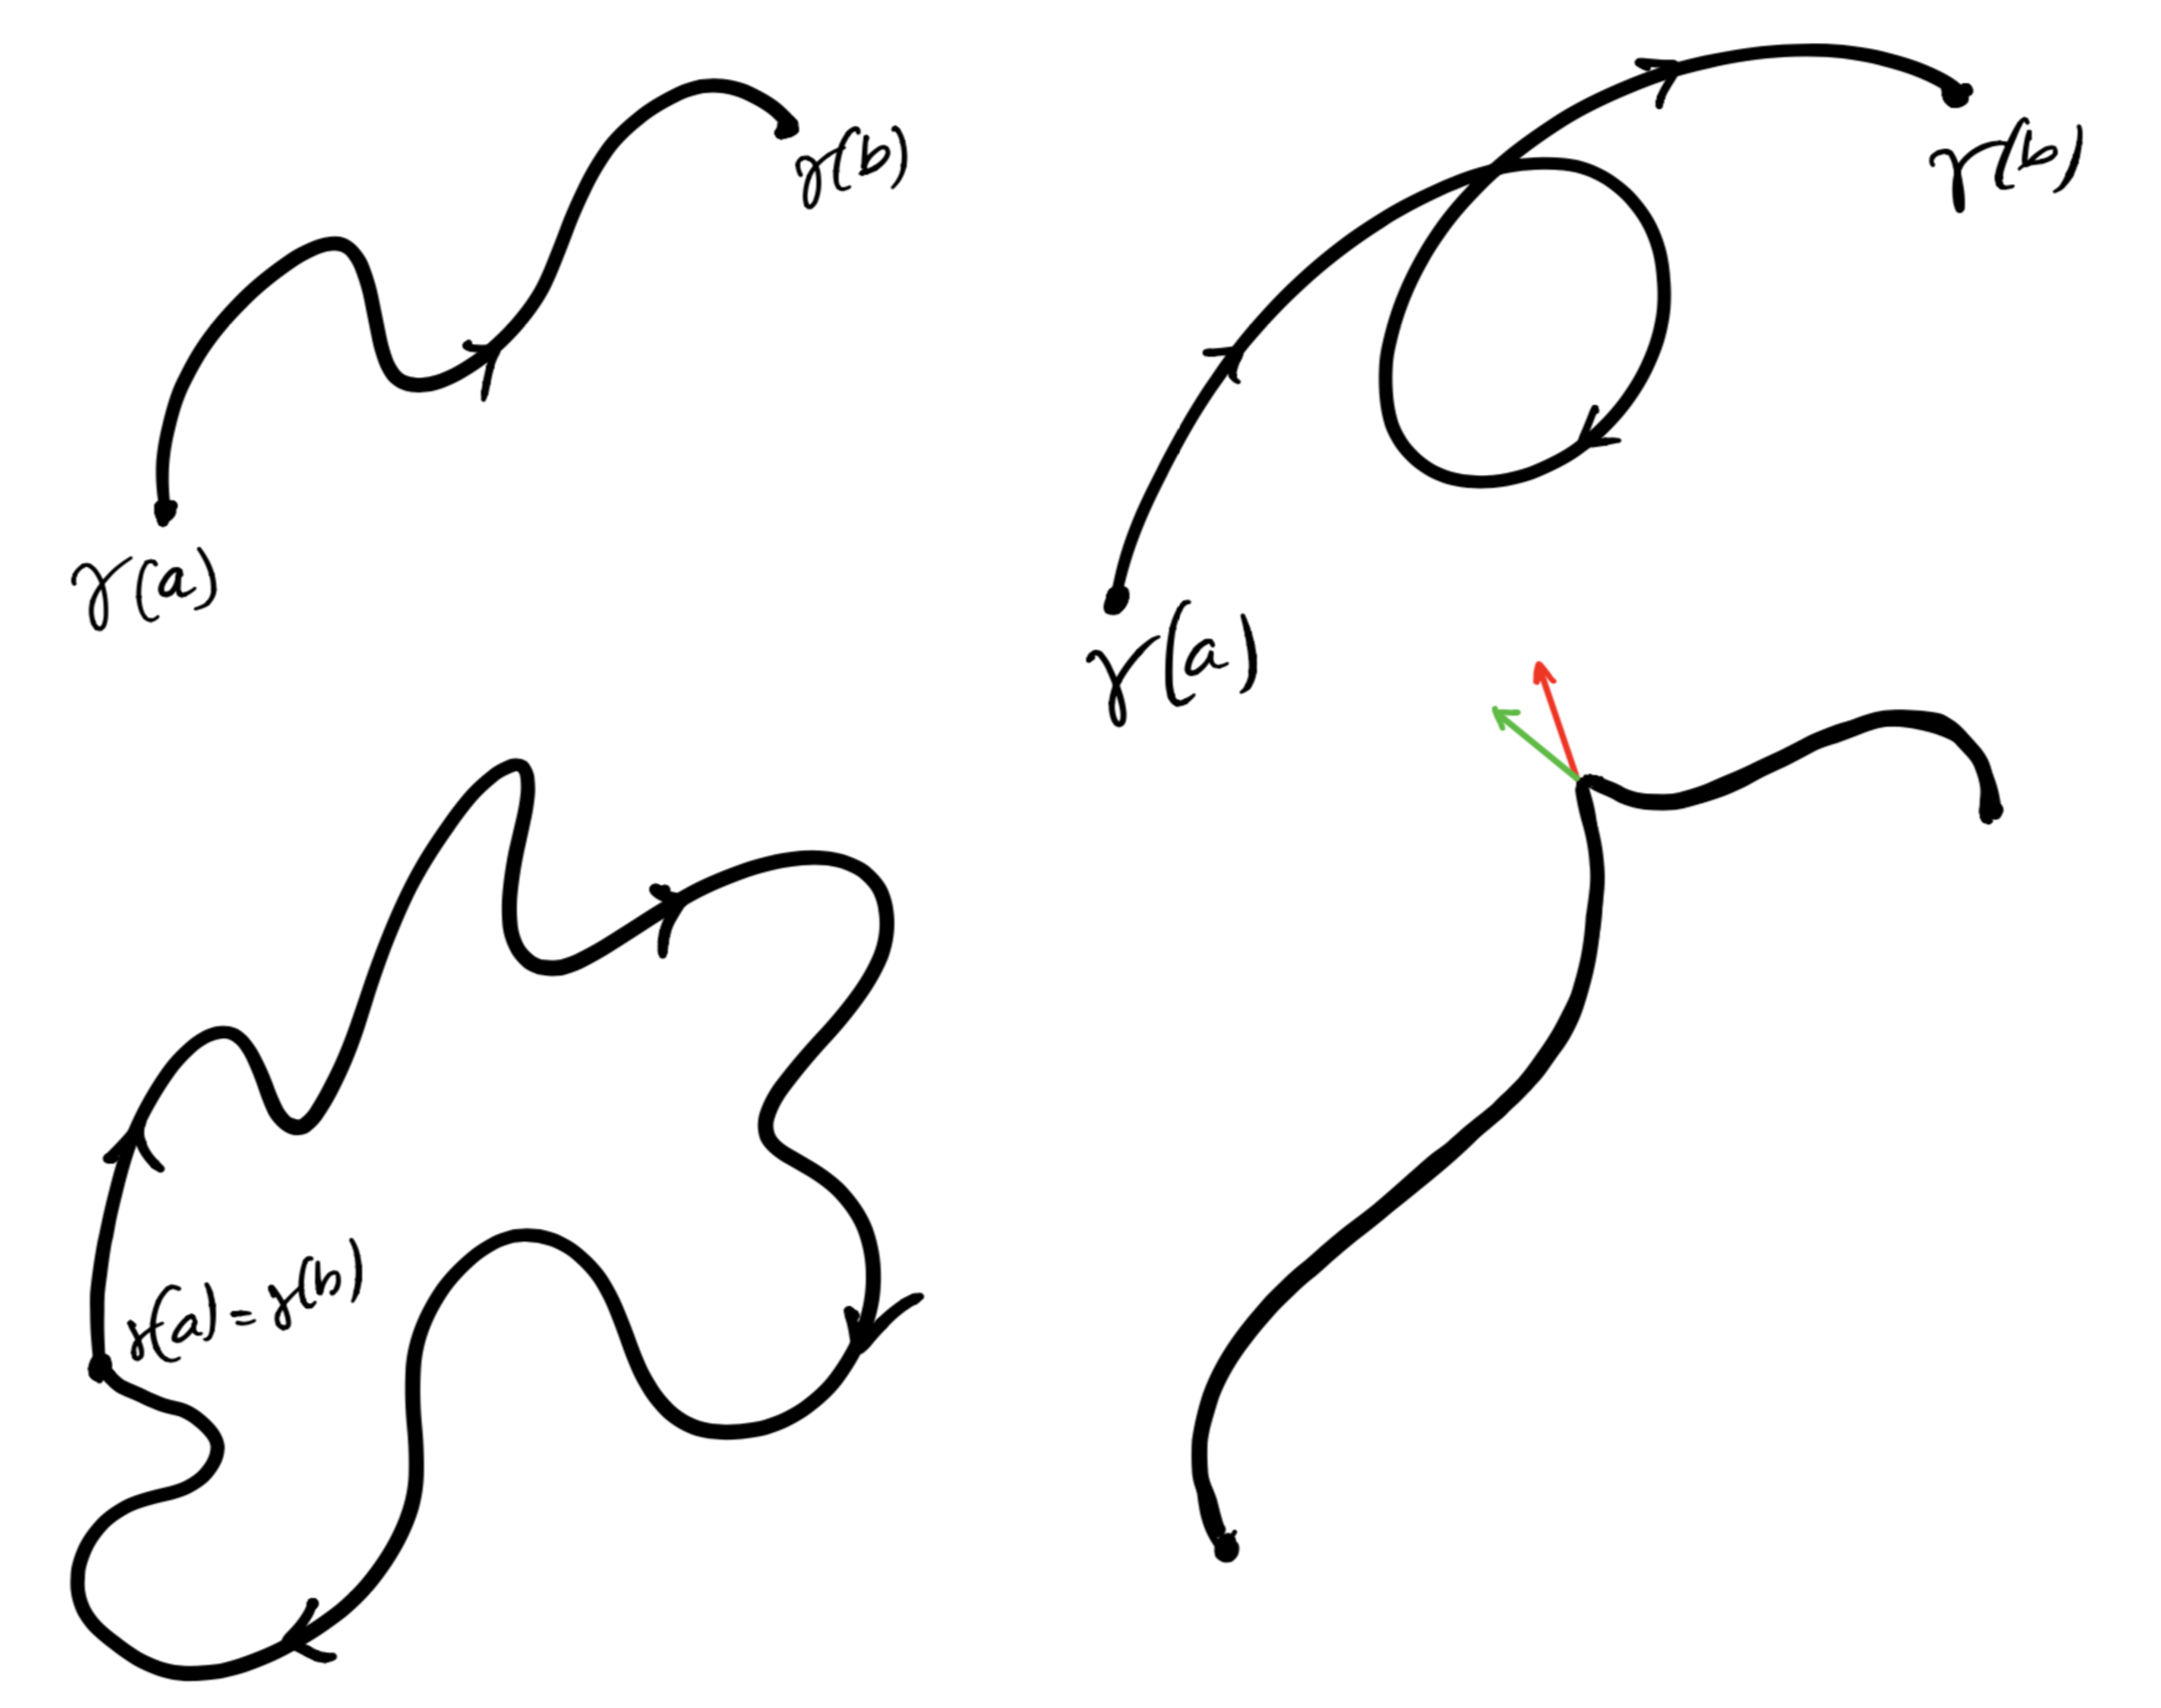
\includegraphics[width=0.9\linewidth]{assets/paths.png}
  \caption{Im Uhrzeigersinn von oben links: ein einfacher Pfad, ein nicht einfacher Pfad; ein nicht differenzierbarer einfacher Pfad und ein geschlossener Pfad.}
\end{figure}

\begin{mainbox}{Kurvenintegral entlang eines Pfades}
  Sei \(U \subseteq \mathbb{C}\) offen, \(f \colon U \to \mathbb{C}\) stetig und sei \(\gamma \colon [0,1] \to U \subseteq \mathbb{C}\) differenzierbar. Wir definieren das Kurvenintegral von \(f\) entlang \(\gamma\) durch:
  
  \begin{align*} 
  \int_{\gamma} f(z) \text{dz} :=& \int_0^1 f(\gamma(\text{t}))\cdot \gamma'(\text{t}) \text{dt}\\
   = &\int_0^1 \Re(f(\gamma (t))  \gamma'(t) )\text{dt} + i \int_0^1 \Im(f(\gamma (t))  \gamma'(t)) \text{dt}
  \end{align*}
\end{mainbox}

\begin{subbox}{Eigenschaften des Kurvenintegrales}
   Sei $\gamma: [0, 1] \mapsto U \subseteq \C$ ein Pfad und \(f\colon U\to\mathbb{C}\) stetig:

  \begin{enumerate}
    \item{
      \textbf{Linearität}: Sei \(g\colon U\to\mathbb{C}\) stetig und \(\alpha,\beta \in \mathbb{C}\). Dann gilt \begin{align*} \int_{\gamma} [ \alpha f(z) + \beta g(z) ] dz = \alpha \int_{\gamma} f(z)dz + \beta \int_{\gamma} g(z)dz\,. \end{align*}
    }
    \item{
      Sei \(\delta\colon[0,1]\to U\subseteq\mathbb{C}\) durch \(\delta(t):=\gamma(1-t)\) definiert. Dann ist \begin{align*} \int_{\delta} f(z) dz =-\int_{\gamma} f(z) dz\,. \end{align*}
 
      Man schreibt \(\delta=\gamma^{-1}\) oder manchmal auch \(\delta=-\gamma\).
    }
    \item{
      Sei \(\delta\colon[0,1]\) ein Pfad mit \(\gamma (1) = \delta(0)\) und setze:
      \begin{align*} (\gamma * \delta) (t) := \begin{cases} \gamma(2t) &\text{ falls } 0 \leq t \leq 1/2\\ \delta (2t-1) &\text{ falls } 1/2 \leq t \leq 1\,. \end{cases} \end{align*}

      $(\gamma * \delta)$ entspricht den Pfaden $\gamma$ und $\delta$ ''aneinander gesetzt''. So gilt:
      \begin{align*} \int_{\gamma * \delta} f(z) dz = \int_{\gamma} f(z) dz + \int_{\delta} f(z) dz\,. \end{align*}
    }
    \item{
      \textbf{Unabhängigkeit der Parameterisierung}: Sei \(\sigma \colon [0,1] \to [0,1]\) eine differenzierbare Funktion mit \(\sigma(0) =0, \sigma(1)=1\) und sei \(\delta\colon[0,1]\to U\) durch \(\delta (t) := \gamma (\sigma (t))\) definiert. Anders gesagt, ist \(\delta\) eine andere Parameterisierung des Bildes von \(\gamma\). Dann gilt:
      \begin{align*} \int_{\delta} f(z)dz=\int_{\gamma} f(z) dz\,. \end{align*}
    }
  \end{enumerate}
\end{subbox}

\begin{mainbox}{Wegzusammenhängend}
  Eine Menge $U$ heisst \textbf{wegzusammenhängend}, falls es für jede zwei Punkte $z_1, z_2 \in U$ einen Pfad gibt, der die zwei Punkte verbindet.
\end{mainbox}

\begin{mainbox}{Stammfunktion}
  Sei \(U \subseteq \mathbb{C}\) eine offene wegzusammenhängende Menge und \(f \colon U \to \mathbb{C}\) stetig. Dann sind folgende Aussagen äquivalent:

  \begin{itemize}
    \item Für jede geschlossene Kurve \(\gamma \colon [0,1] \rightarrow U\) gilt \(\int_{\gamma} f(z) dz = 0\).
    \item Das Kurvenintegral \(\int_\delta f(z)dz\) ist unabhängig vom Pfad \(\delta\colon[0,1]\to U\).
    \item Es gibt eine \(\mathbb{C}\)-differenzierbare Funktion \(F \colon U \to \mathbb{C}\) mit \(F'(z)=f(z)\).
  \end{itemize}

Falls eine (und deshalb jede) der Aussagen gilt, heisst die Funktion \(F\) eine Stammfunktion von \(f\) und \begin{align*} \int_\delta f(z)\,dz=F(\delta(1))-F(\delta(0))\,. \end{align*}

\end{mainbox}

Aus dem Cauchy'schen Integralsatz erhalten wir eine Behauptung wann die obigen Aussagen gelten.

\subsection{Cauchy'scher Integralsatz}

\begin{subbox}{Homotopie}
  Sei \(U \subseteq \mathbb{C}\) offen, \(\gamma_0, \gamma_1: [a,b] \to U\) Pfade mit \(\gamma_0(a) = \gamma_1(a)=\alpha\) und \(\gamma_0(b) = \gamma_1(b)=\beta\). Wir sagen \(\gamma_0\) sei homotop zu \(\gamma_1\), falls es eine stetige Funktion \(H \colon [0,1]\times[a,b] \to U\) mit:
  
  \begin{equation*}
    \begin{matrix} H(0,t) = \gamma_0(t)\\ H(1,t) = \gamma_1(t) 
    \end{matrix} ~~~ \forall t \in [a,b] ~~~ \text{ und } ~~~ \begin{matrix} H(s,a)=\alpha\\ H(s,b) = \beta \end{matrix} ~~~ \forall s\in [0,1] \end{equation*} gibt. Die Funktion \(H\) ist die sogennante Homotopie von \(\gamma_0\) und \(\gamma_1\).

\end{subbox}

Dies definiert eine stetige Deformation $H$ von $\gamma_0$ zu $\gamma_1$. Für jedes feste $s \in [0,1]$ ist $\gamma_s(t) := H(s, t)$ ein Pfad von $\alpha$ nach $\beta$, definiert auf $[a,b]$. Eine Homotopie kann z.B. durch die Parameterisierung $H(s, t) = (1 - s)\gamma_1(t) + s \gamma_2(t)$ gefunden werden.

\begin{subbox}{einfach zusammenhängend}
  Eine teilmenge $U \subseteq \C$ heisst \textbf{einfach zusammenhängend} falls sie wegzusammenhängend ist und für alle $\alpha, \beta \in U$, alle Pfade von $\alpha$ nach $\beta$ homotop zu einander sind.
\end{subbox}

\begin{figure}[H]
  \centering 
  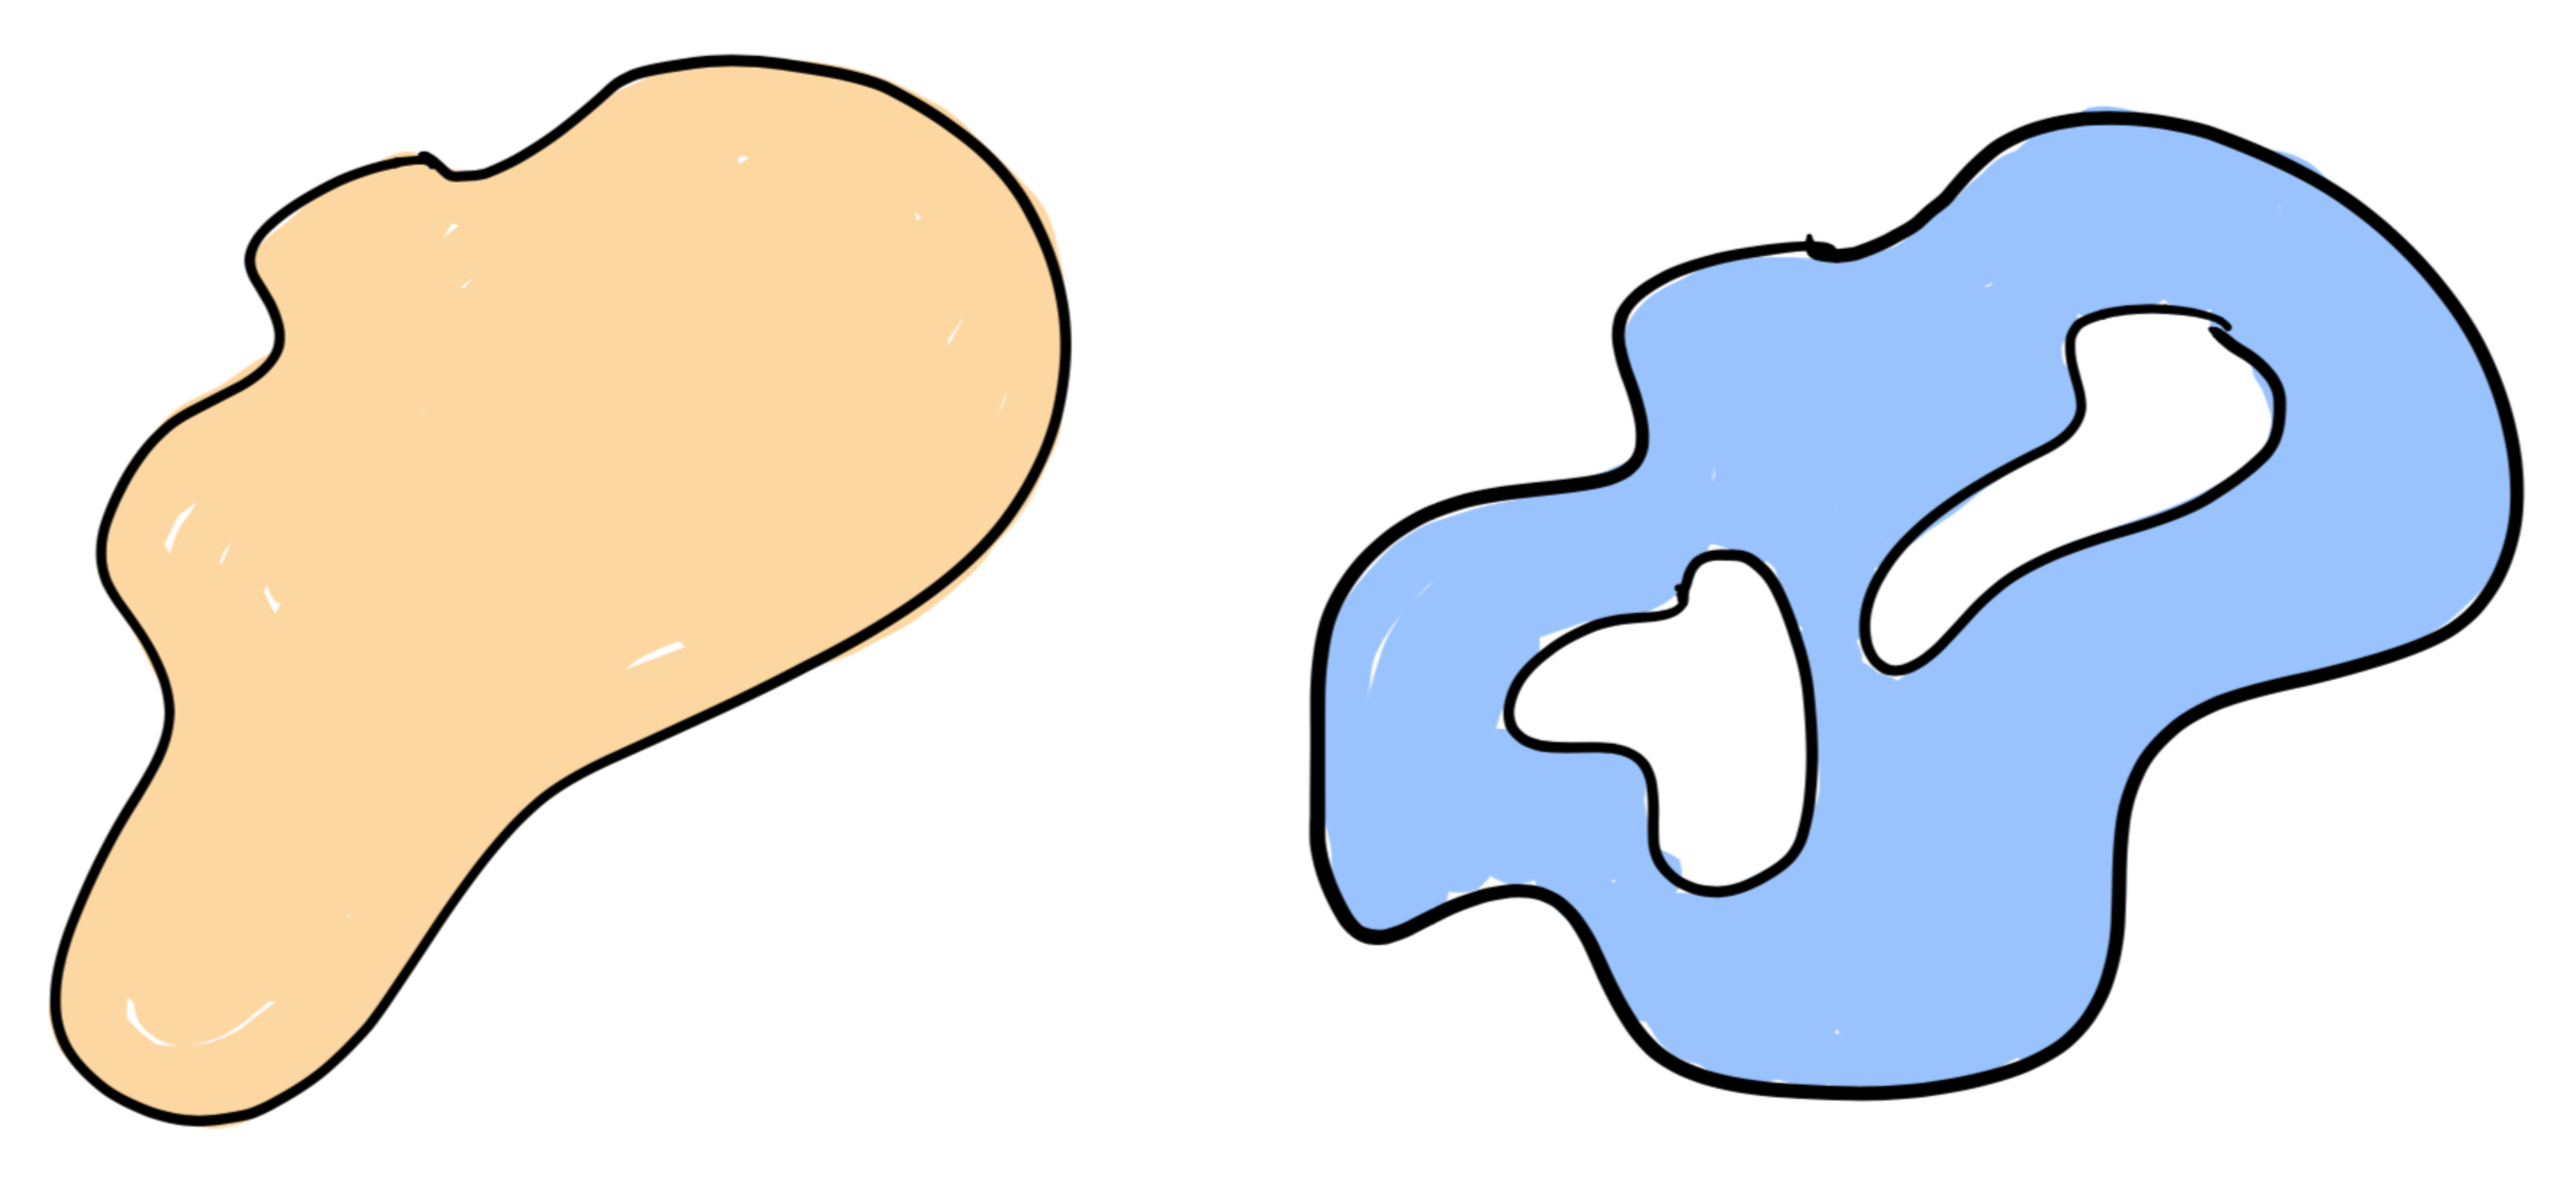
\includegraphics[width=0.9\linewidth]{assets/connected.png}
  \caption{Eine einfach zusammenhängende Menge an der linken Seite und eine nicht einfach zusammenhängende Menge an der rechten Seite.}
\end{figure}

\begin{mainbox}{Cauchy'scher Integralsatz}
  Sei $U \subseteq \C$ eine einfach zusammenhängende offene Teilmenge und $f: U \mapsto \C$ eine holomorphe Funktion. Dann besitzt $f$ eine Stammfunktion auf $U$.
\end{mainbox}

Aus den drei äquivalenten Aussagen folgt nun:

\begin{subbox}{Konsequenzen des Cauchy'schen Integralsatzes}
  Sei $U \subseteq \C$ eine einfach zusammenhängende offene Teilmenge und $f: U \mapsto \C$ eine holomorphe Funktion.
  \begin{itemize}
    \item Sei $\gamma$ ein geschlossener Pfad. Dann gilt $\int_\gamma f(z) dz = 0$.
    \item Das Kurvenintegral von $f$ ist unabhängig vom Pfad.
  \end{itemize}
\end{subbox}

\begin{mainbox}{Eigenschaften (I)}
  Sei \(U\subseteq\mathbb{C}\) eine wegzusammenhängende Menge, sei \(\gamma\colon[a,b]\to U\) ein Pfad und \(f\colon U\to\mathbb{C}\) stetig. Dann gilt:

  \begin{itemize}
    \item{
      Dreiecksungleichung für Weg-Integrale:
      \begin{align*}\left|\int_a^b f(\gamma (t)) \cdot \gamma'(t) \,dt\right| \leq \int_a^b \left|f(\gamma (t))\cdot \gamma'(t)\right|\, dt\, .\end{align*}
    }
    \item{
      Sei \(L\) die Länge von \(\gamma\), d.h. \(L=\int_a^b|\gamma'(t)|dt\). Wenn \(|f(z)| \leq M\) für jedes \( z\in U\), dann folgt \begin{align*} \left|\int_{\gamma} f(z)dz\right| \leq M\cdot L \end{align*}
    }
  \end{itemize}
\end{mainbox}

\begin{mainbox}{Eigenschaften (II)}
  \begin{enumerate}
    \item Sei \(\gamma\) eine geschlossene einfache im Gegenuhrzeigersinn orientierte Kurve.
    \item Seien \(\gamma_1,\dots,\gamma_n\) einfache geschlossene im Uhrzeigersinn orientierte Kurven, die innerhalb \(\gamma\) sind. Nehmen wir an, dass die Mengen, die diese Kurven einschliessen, keine Schnittpunkte mit einanderen haben.
    \item Sei \(U\) die Menge von diesen Kurven definiert.
  \end{enumerate} 

  \begin{figure}[H]
    \centering 
    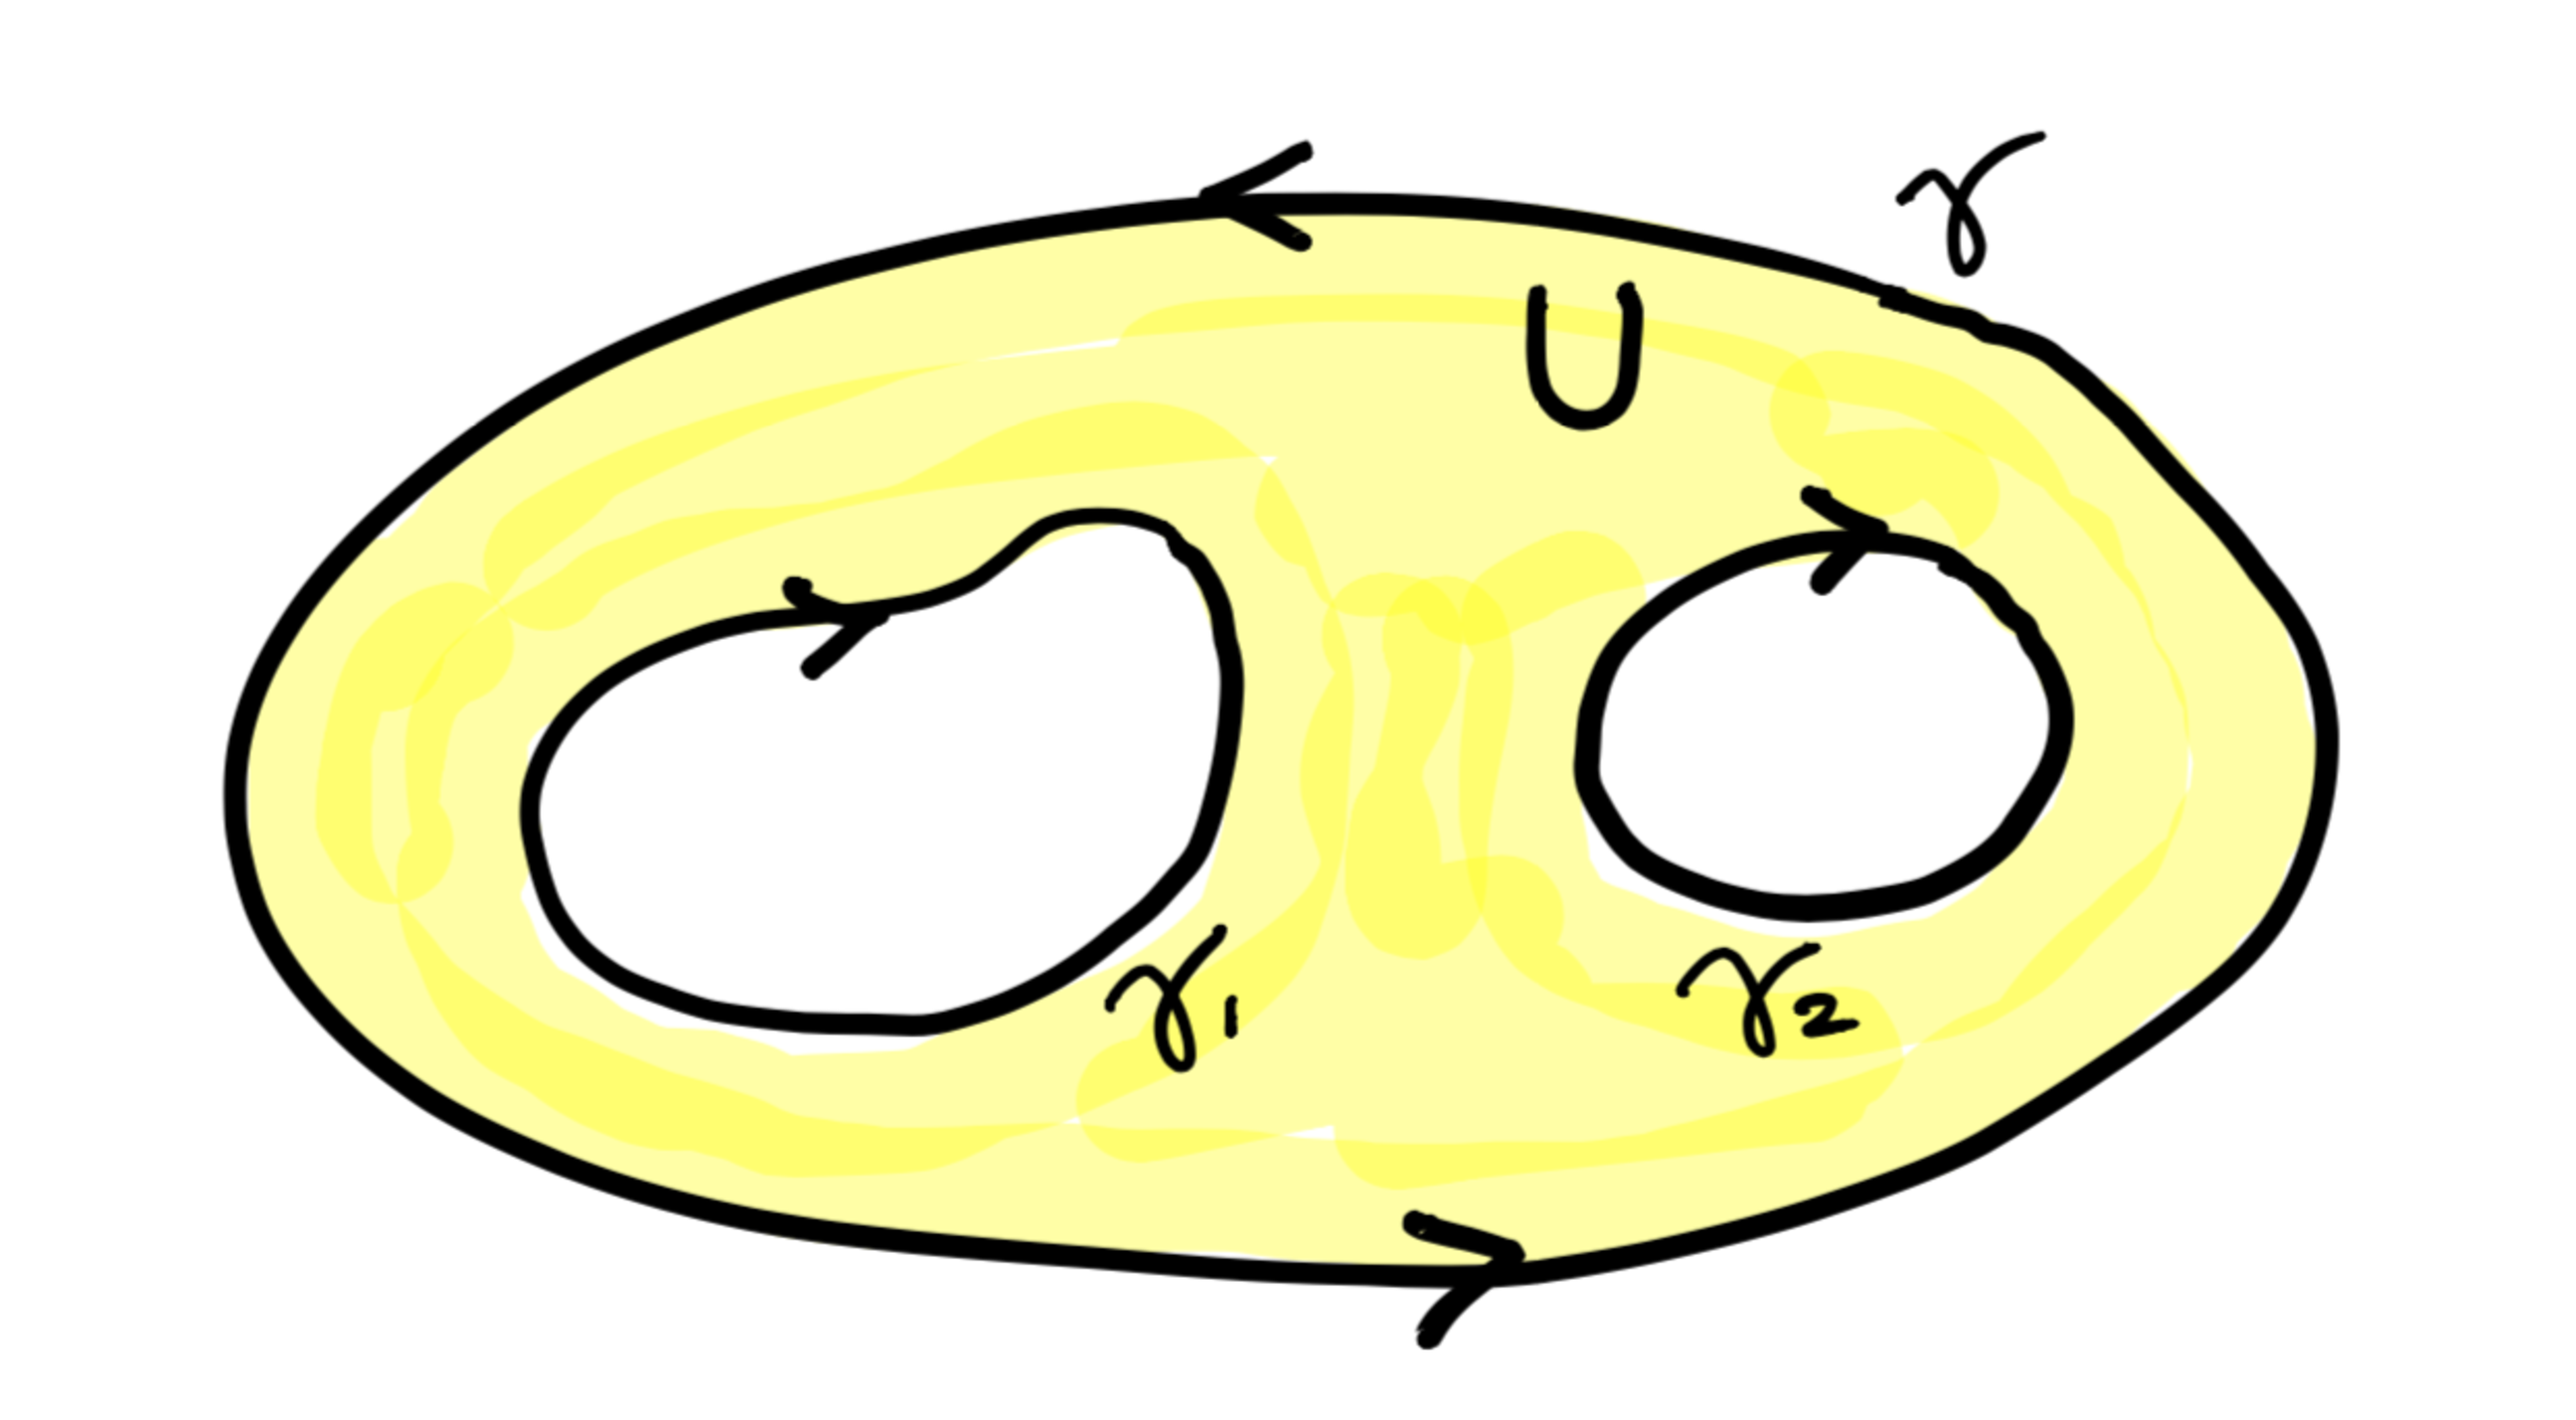
\includegraphics[width=0.6\linewidth]{assets/3-4-1.png}
  \end{figure}
  
  Falls \(f\colon U\to\mathbb{C}\) holomorph ist, gilt:
  \begin{align*} \int_\gamma f(z)\,dz+\sum_{k=1}^n\int_{\gamma_k}f(z)\,dz=0 \end{align*}
\end{mainbox}

Insbesondere, seien \(\gamma_1\) und \(\gamma_2\) zwei Kurven mit der gleichen Orientierung und sei \(U\) als die Menge von diesen zwei Kurven definiert. Falls \(f\colon U\to\mathbb{C}\) holomorph ist, gilt \begin{align*} \int_{\gamma_1}f(z)\,dz=\int_{\gamma_2}f(z)\,dz\,. \end{align*}

\subsection{Mittelwertsatz, Maximum Prinzip und Satz von Liouville}

\begin{mainbox}{Cauchy'sche Integralformel}
  Sei \(U \subseteq \mathbb{C}\) eine einfach zusammenhängende offene Menge und \(z_0\in U\). Sei \(\gamma \colon [0,1] \to U \setminus \{z_0\}\) eine Kurve, die \(z_0\) einmal im positiven Sinn umläuft und sei \(f \colon U \to \mathbb{C}\) holomorph. Dann gilt:
\begin{align*}f(z_0) = \frac{1}{2\pi i} \int_{\gamma} \frac{f(z)}{z-z_0}dz \end{align*}
\begin{figure}[H]
  \centering 
  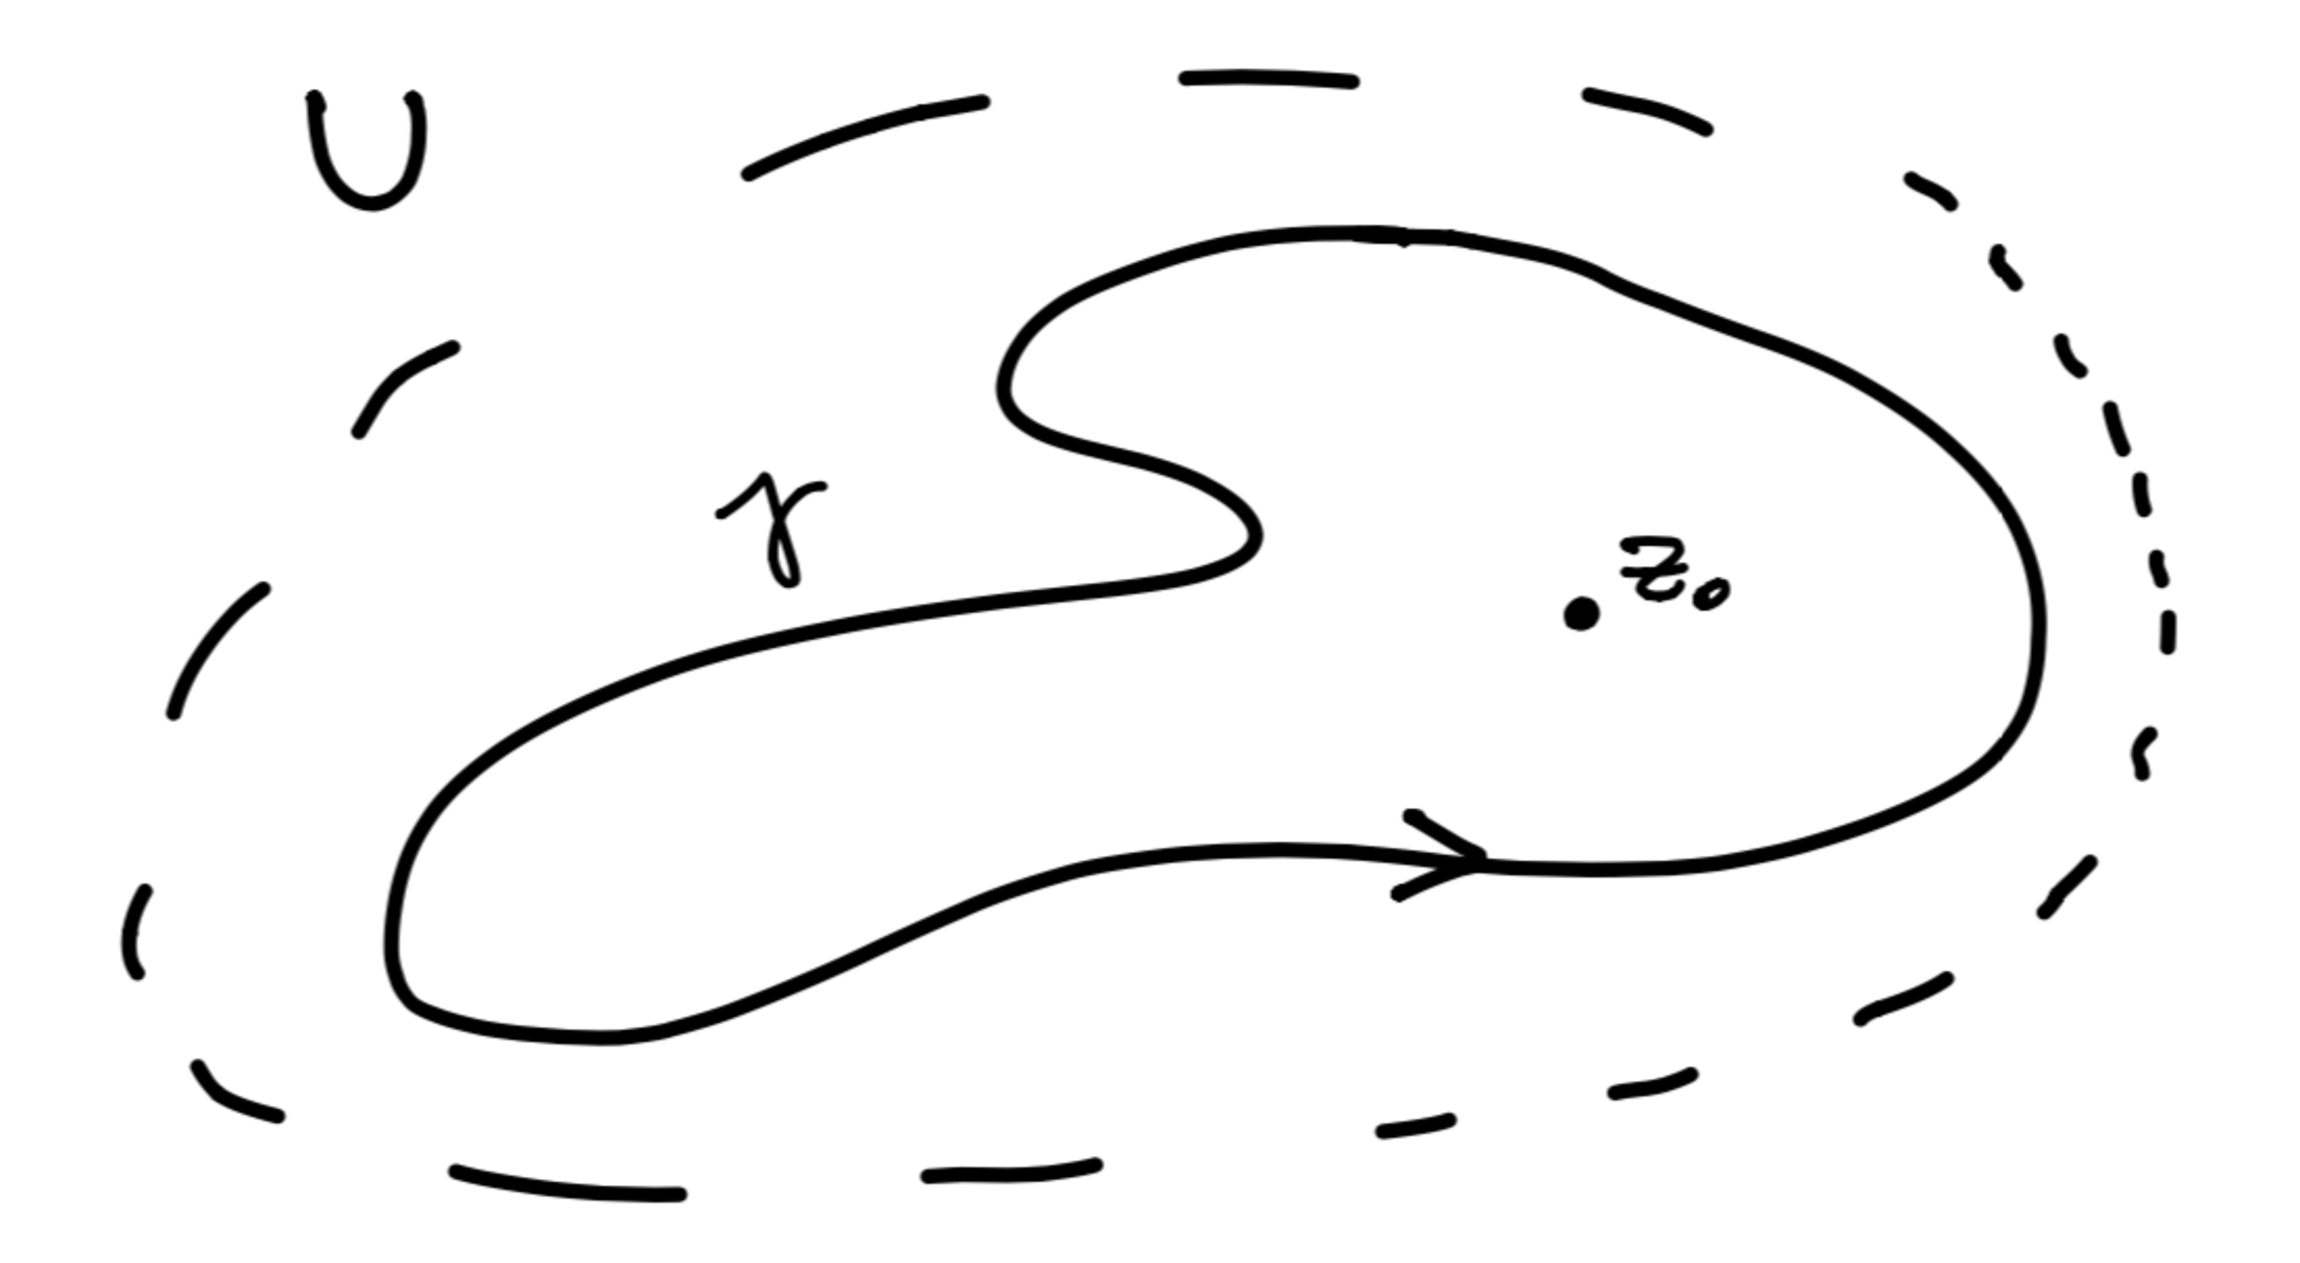
\includegraphics[width=0.6\linewidth]{assets/3-5-1.png}
\end{figure}
\end{mainbox}

Mit dieser Formel können wir z.B. das Integral $\int_\gamma \frac{z}{(9-z^2)(z+i)} dz$ und $\gamma(t) = 2\exp(2\pi it)$ einfacher berechnen. Definieren wir $f(z) := \frac{z}{9 - z^2}$, so gilt:
\begin{align*}
  \int_\gamma \frac{z}{(9-z^2)(z+i)} dz = \int_\gamma \frac{f(z)}{z + i} dz = 2\pi i f(-i)
\end{align*}

Durch Induktion folgt auch:

\begin{mainbox}{Verallgemeinerung von Cauchy's Integralsatz}
  Sei \(f \colon U \to \mathbb{C}\) mit \(U\subseteq \mathbb{C}\) offen, holomorph, so ist \(f\) beliebig oft \(\mathbb{C}\)-differenzierbar und es gilt für \(z_0\in U\) und eine beliebige Kurve \(\gamma \colon [0,1] \to U\) die \(z_0\) einmal im Gegenuhrzeigersinn umrundet: \begin{align*} f^{( n )}(z_0) = \frac{n!}{2\pi i} \int_{\gamma} \frac{f(z)}{(z-z_0)^{n+1}}dz \end{align*}
\end{mainbox}

Daraus folgt nun:

\begin{subbox}{Differenzierbarkeit holomorpher Funktionen}
  Sei $f$ holomorph. Dann sind alle Ableitungen $f^{(n)}$ holomorph.

  Weiter, sei $u := \Re(f), v := \Im(f)$, so haben $u, v$ unendlich viele partielle Ableitungen.
\end{subbox}

\begin{mainbox}{Mittelwertsatz}
  Seien \(U\subset\mathbb{C}\) eine offene Menge und \(f \colon U \to \mathbb{C}\) eine holomorphe Funktion. Seien \(z_0 \in U\) und \(r > 0\) so dass \(\overline{B(z_0,r)} \subseteq U\). Dann gilt:
  \begin{align*} f(z_0) = \int_0^1 f(z_0 + r \exp(2 \pi i t))\, dt\,, \end{align*} d.h.\(f(z_0)\) ist der Mittelwert von \(f\) auf dem Kreis mit Zentrum \(z_0\) und Radius \(r\).
\end{mainbox}

Aus dem Mittelwertsatz schliessen wir nun:

\begin{subbox}{Maximum holomorpher Funktionen}
  Sei $f$ auf $B(z_0, r)$ holomorph. Falls $|f(z)| \leq |f(z_0)|$ für jedes $z \in B(z_0, r)$ gilt, dann ist:
  $$
    f(z) = f(z_0)
  $$

  Das heisst $f$ ist konstant (da $|f|$ konstant und $f$ holomorph).
\end{subbox}

Daraus folgt wiederum per Widerspruchsbeweis:

\begin{mainbox}{Maximum Modulus Prinzip}
  Sei $f$ holomorph und nicht konstant auf einer wegzusammenhängenden offenen Menge $U$. Dann besitzt $|f(z)|$ \textbf{kein} Maximum auf $U$.
\end{mainbox}

Im obigen Satz gibt es also keinen Punkt $z_0 \in U$ mit $|f(z)| \leq |f(z_0)|$. Dasselbe gilt auch für das \textbf{Minimum}.

\begin{subbox}{Maximum auf kompakter Menge}
  Sei $f$ eine nicht-konstante, stetige Funktion auf  einer kompakten Menge $K$. Sei $f$ holomorph auf dem Inneren von $K$. Dann wird $\max_{z \in K} |f(z)|$ auf dem Rand von $K$ erreicht.
\end{subbox}

\begin{mainbox}{Satz von Liouville}
  Sei $f: \C \mapsto \C$ eine ganze Funktion (also definiert und holomorph auf der ganzen komplexen Ebene). Falls $|f(z)|$ beschränkt ist, so ist $f$ konstant.
\end{mainbox}

Der Satz von Liouville gilt nicht für Funktionen die nur auf einer reellen Variable definiert sind. Beispielsweise $f(x, y) = \cos(x) \sin(y)$ ist auf der ganzen reellen Ebene beschränkt und unendlich oft differenzierbar, aber nicht konstant.

\section{Taylor- und Laurentreihen}

\subsection{Reihen Entwicklung}

\begin{mainbox}{Komplexe Taylorreihe}
  Sei \( f \colon B(z_0,R_0) \to \mathbb{C}\) eine holomorphe Funktion und \( R_0 > 0 \). Dann besitzt \(f\) eine Reihen Entwicklung so dass für jedes  \(z\in B(z_0,R_0)\) gilt: \begin{align*} f(z) = \sum_{n=0}^{\infty} \frac{f^{( n )}(z_0)}{n!} (z-z_0)^n \end{align*} Anders gesagt, die Reihe konvergiert absolut für alle \( z\in B(z_0,R_0)\).
\end{mainbox}

Falls $z_0 = 0$, nennt man die Reihe \textbf{MacLaurin}-Reihe von $f$. 

\begin{subbox}{Geometrische Reihe}
  Falls $|z| < 1$ gilt:
  $$
    \frac{1}{1 - z} = \sum_{n=0}^\infty z^n
  $$
  Für die Partialsumme gilt $S_n = \frac{1 - z^{n+1}}{1 - z}$.
\end{subbox}

\begin{mainbox}{Laurentreihe}
  Sei \(f\) eine Funktion, die holomorph auf einem Kreisring \( R_1 <|z-z_0| < R_2 \) ist. Dann besitzt \(f\) für jedes \(z\) im Kreisring eine Reihen Entwicklung:
  \begin{align*} f(z)=\sum_{n=0}^\infty a_n(z-z_0)^n+\sum_{n=1}^\infty b_n\frac{1}{(z-z_0)^n}\end{align*}
  wobei:
  \begin{align*} a_n=\frac{1}{2\pi i}\int_\gamma\frac{f(z)}{(z-z_0)^{n+1}}\,dz\,,\text{ für } n=0,1,2,\dots\end{align*} \begin{align*}b_n=\frac{1}{2\pi i}\int_\gamma\frac{f(z)}{(z-z_0)^{-n+1}}\,dz\,,\text{ für } n=1,2,\dots \end{align*} und \(\gamma\) ist eine geschlossene Kurve, die im Kreisring enthalten ist und die einmal im Gegenuhrzeigersinn \(z_0\) umläuft.
\end{mainbox}

\begin{figure}[H]
  \centering 
  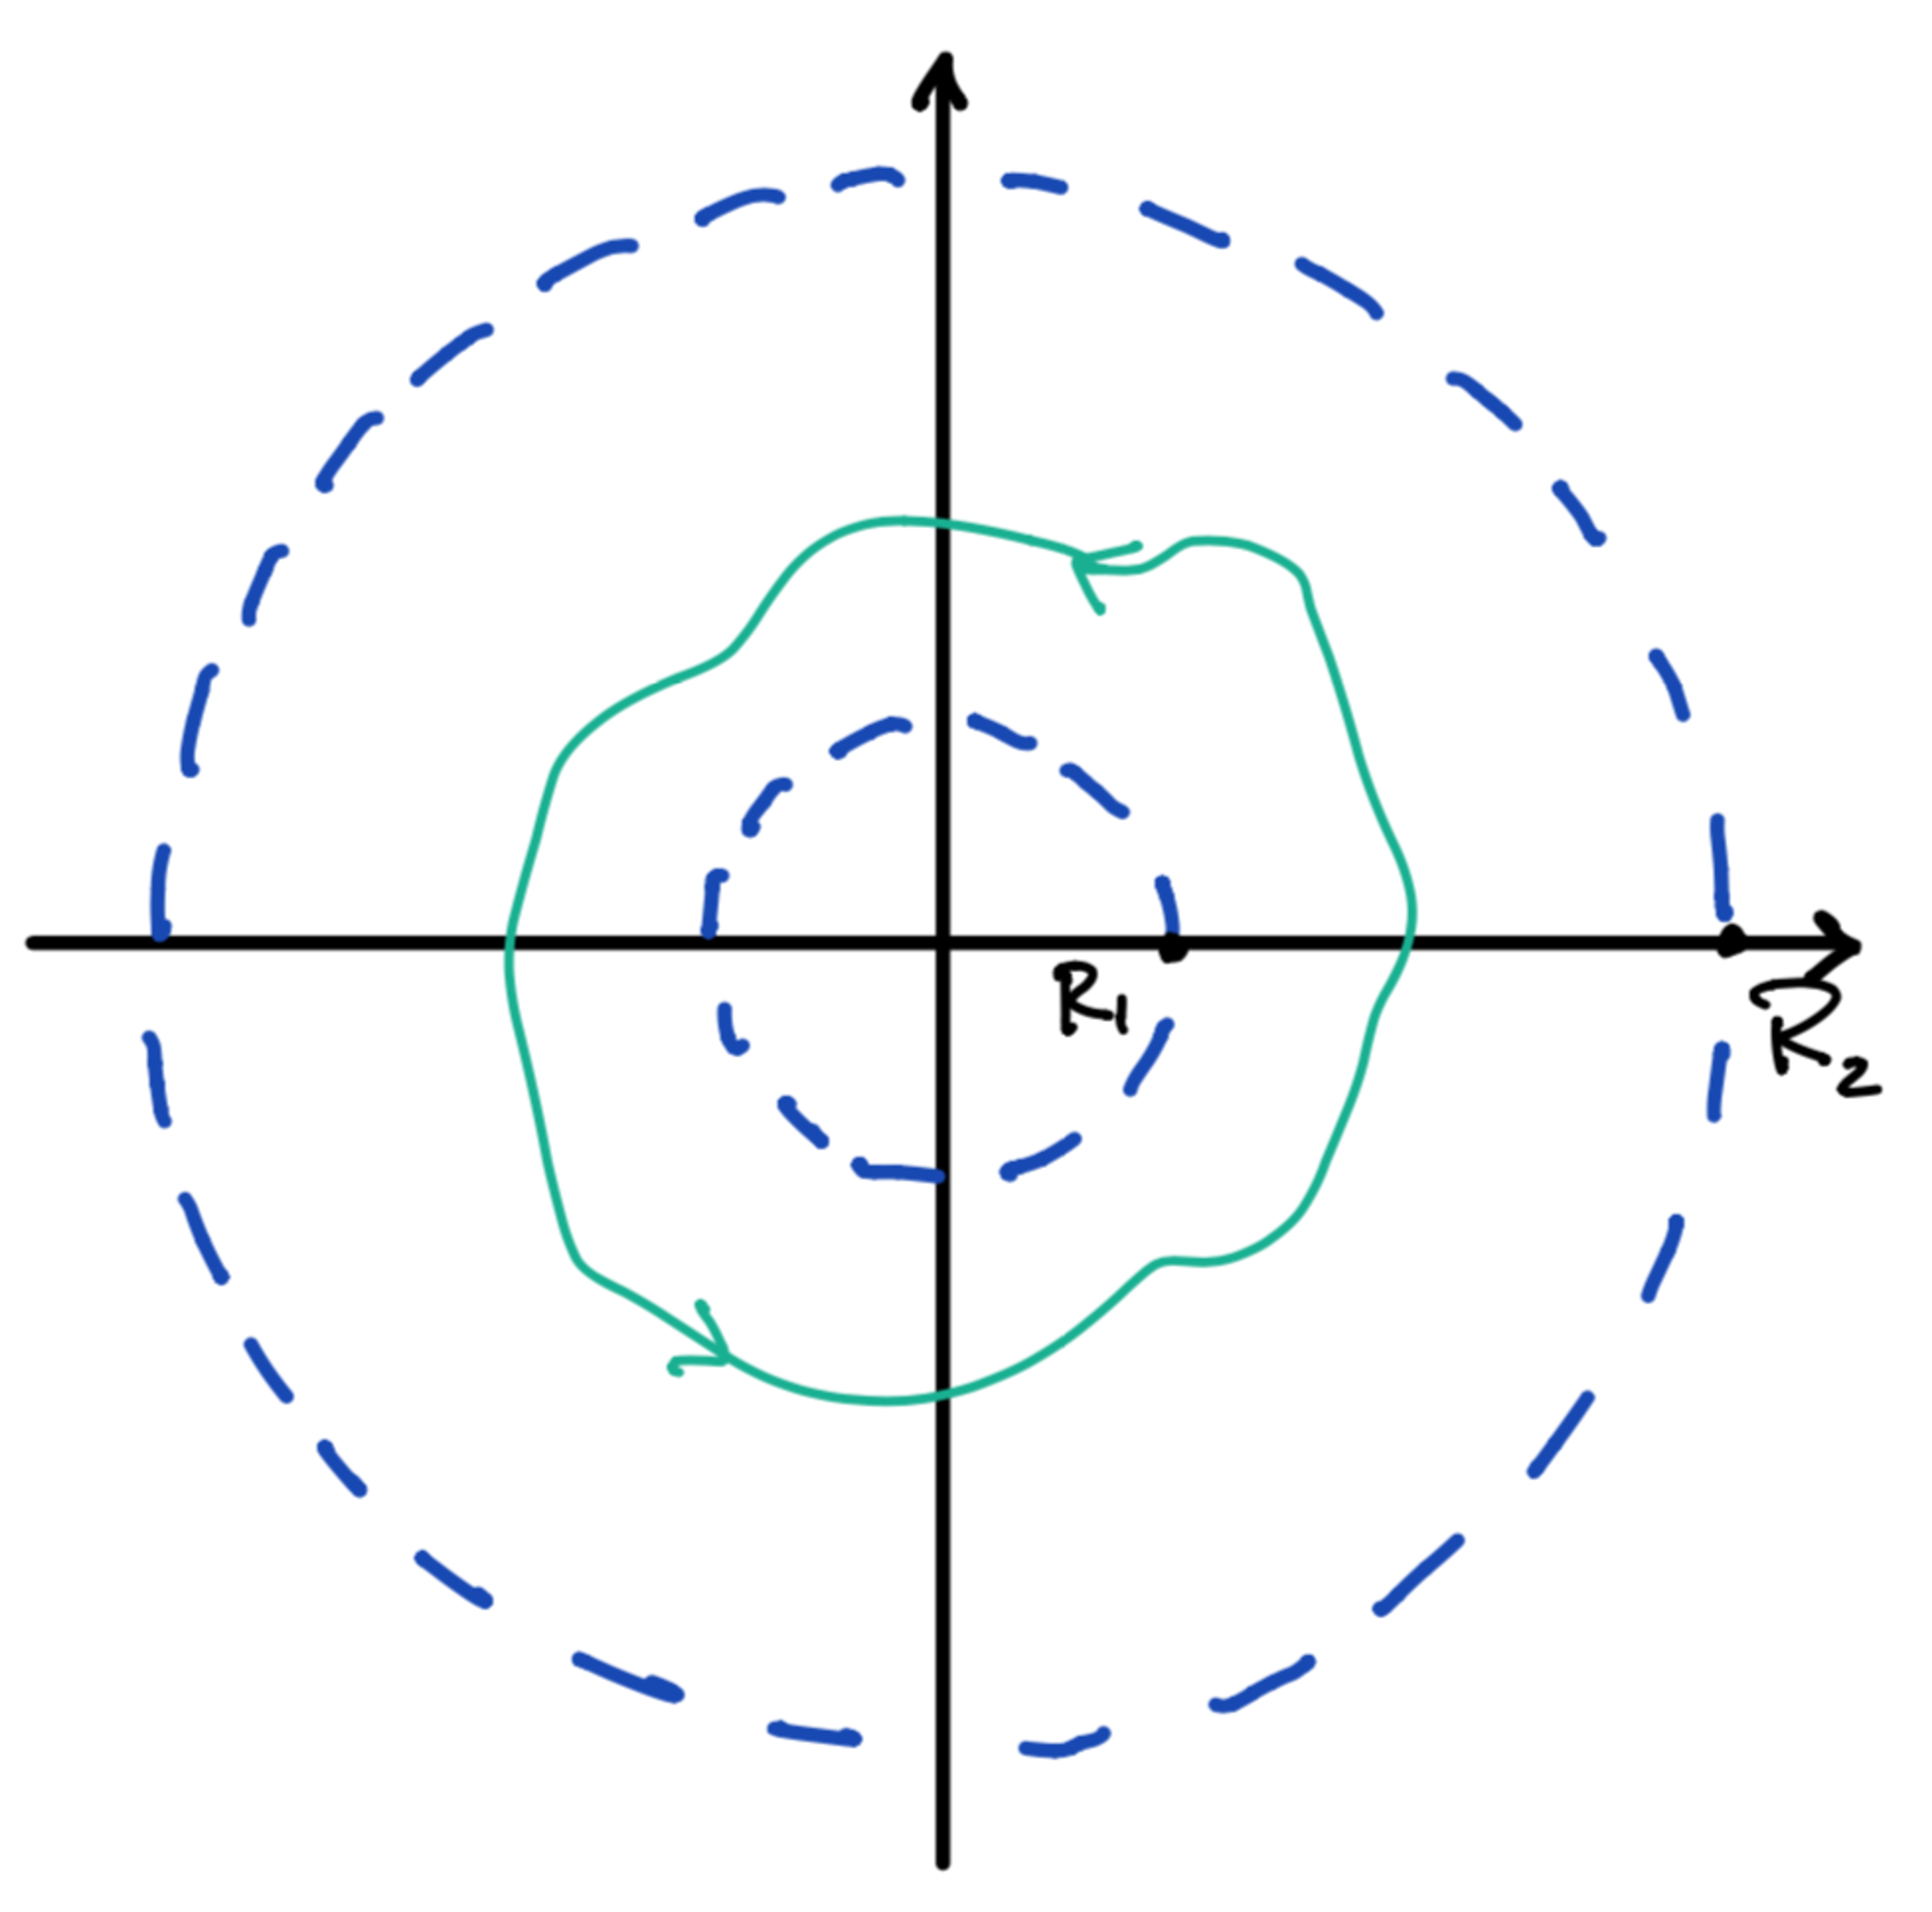
\includegraphics[width=0.4\linewidth]{assets/4-1-1.png}
  \caption{Kreisring für Kurve bei Laurentreihe}
\end{figure}

\begin{enumerate}
  \item{
    Die Laurentreihe lässt sich auch in einer \textbf{kompakteren Form} schreiben:

    \begin{align*} 
       f(z) = \sum_{n=-\infty}^{\infty} c_n (z-z_0)^n
     \end{align*}
     wobei:
     \begin{align*}
      c_n=\frac{1}{2\pi i}\int_\gamma\frac{f(z)}{(z-z_0)^{n+1}}\,dz\,,\text{ für } n=0,\pm1,\pm2,\dots
    \end{align*}
  }

  \item{
    Die Formel für \(b_n\) kann auch als 
    \begin{align*} b_n=\frac{1}{2\pi i}\int_\gamma f(z)(z-z_0)^{n-1}\,dz\,,\text{ für } n=1,2,\dots \end{align*} geschrieben werden. Falls \(f\) an der Stelle \(z_0\) holomorph ist, ist die Funktion \(f(z)(z-z_0)^{n-1}\) auch holomorph und \(b_n=0\) für \(n=1,2,\dots\). In diesem Fall ist die Laurent-Reihen Entwicklung die Taylor-Reihen Entwicklung und \begin{align*} a_n=\frac{1}{n!}f^{( n )}(z_0) \end{align*}
  }
\end{enumerate}

\begin{subbox}{Analytische Funktion}
  Eine Funktion heisst analytisch, falls sie sich durch eine Potenzreihe darstellen lässt.
\end{subbox}

\begin{subbox}{Singularitäten und Nullstellen}
  Man nennt \(z_0\) eine isolierte \textbf{Singularität} der Funktion \(f\), wenn \(f\) an der Stelle \(z_0\) nicht holomorph ist, aber es ein \(\epsilon>0\) gibt, so dass \(f(z)\) für jedes \(z\in B(z_0,\epsilon)\setminus \{ z_0 \}\) holomorph ist.
  
  Eine Nullstelle \(z_0\) einer Funktion heisst \textbf{isoliert}, falls es ein \(\epsilon>0\) gibt, so dass für jedes \(z\in B(z_0,\epsilon)\) : \(f(z)\neq0\).
\end{subbox}

Die Funktion $f(z) = |z|^2$ hat bspw. keine Singularitäten, weil sie nirgendwo holomorph ist.

\begin{mainbox}{Klassifizierung von Singularitäten und Nullstellen}
  Sei \(U\subseteq \mathbb{C}\) offen, \(z_0 \in U\) und \(f\) holomorph auf \(U\setminus\{z_0\}\). Wir schreiben \(f(z) = \sum_{n=-\infty}^{\infty} c_n (z-z_0)^n\) für jedes \(z\in B(z_0,R)\setminus\{z_0\}\) für ein gewisses \(R>0\). So definiert man:

  \begin{enumerate}
    \item{
      \(z_0\) ist eine \textbf{wesentliche Singularität} falls \(c_n \neq 0\) für unendlich viele negative \(n\).
    }
    \item{
      \(z_0\) ist ein \textbf{Pol der Ordnung \(m \geq 1\)} falls \(c_{-m} \neq 0\) und \(c_n =0\) für alle \(n<-m\). Falls \(m=1\), heisst \(z_0\) ein einfacher Pol.
    }
    \item{
      \(z_0\) ist eine \textbf{hebbare Singularität} falls \(c_n = 0\) für alle \(n<0\).
    }
    \item{
      \(z_0\) ist eine Nullstelle der Ordnung \(m \geq 0\) falls \(c_m \neq 0\) und \(c_n =0\) für alle \(n < m\).
    }
  \end{enumerate}
\end{mainbox}

Falls $z_0$ eine hebbare Singularität von $f$ ist, so kann man $f$ in einer Umgebung von $z_0$ holomorph fortsetzen.

\subsection{Residuensatz}

Sei \(f \colon U \setminus \{ z_0 \} \to \mathbb{C}\) holomorph, so dass man \(f\) als \begin{align*} f(z) = \sum_{n=-\infty}^{\infty} c_n (z-z_0)^n\,, \end{align*} auf einer Scheibe einer gewisses Radius (ausser \(z_0\)) schreiben kann, wobei \begin{align*} c_n = \frac{1}{2\pi i} \int_{\gamma} \frac{f(\xi)}{(\xi - z_0)^{n+1}} d\xi \end{align*} mit \(\gamma \subset U\) eine positiv orientierte geschlossene Kurve ist, die einmal \(z_0\) im positiven Sinne umrundet. Insbesondere gilt für \(n=-1\) \begin{align*}c_{-1} = \frac{1}{2\pi i} \int_{\gamma} f(\xi) d\xi \end{align*}

\begin{mainbox}{Residuum}
  Sei \(z_0\) eine isolierte Singularität von \(f\). Mann nennt den Koeffizienten \(c_{-1}\) von \(\frac{1}{z-z_0}\) in der Laurent-Reihe von \(f\) (entwickelt an $z_0$), das Residuum von \(f\) an der Stelle \(z_0\) und schreibe \(\operatorname{Res}(f,z_0)\).
\end{mainbox}

Man kann Residuen verwenden um komplexe Integrale einfacher zu lösen. Es reicht dazu aus den Koeffizient aus der Laurent-Reihen Entwicklung abzulesen.

Beispielsweise möchten wir $\int_\gamma \exp(\frac{1}{z^2}) dz$ auf der Kurve $\gamma(t) = r \exp(2\pi i t)$ für $r > 0$ berechnen. Eine isolierte Singularität existiert nur im Nullpunkt. Folglich:
$$
\int_\gamma \exp \left( \frac{1}{z^2} \right) dz = 2\pi i \Res(f, 0)
$$
Da $\exp(1/z^2) = \sum_{n=0}^\infty \frac{1}{n!} \frac{1}{z^{2n}}$ können wir ablesen dass $\Res(f, 0) = c_{-1} = 0$.

Für \textbf{gerade Funktionen} gilt dies allgemein: Falls $f(z)$ gerade ist so gilt immer $\Res(f, z_0) = 0$, da die Laurentreihe nur gerade Koeffizienten hat.

\begin{mainbox}{Residuensatz}
  Sei \(U \subseteq \mathbb{C}\) eine offene wegzusammenhängende Teilmenge und sei \(\gamma : [0,1] \to U\) eine positiv orientierte einfache geschlossene Kurve. Seien \(z_1,...,z_n\) im Inneren von \(\gamma\) enthalten und sei \(f \colon U \setminus \{z_1,...,z_n\} \to \mathbb{C}\) holomorph. Dann gilt: \begin{align*}  \int_{\gamma} f(z)\,dz = 2\pi i \sum_{j=1}^n \operatorname{Res}(f,z_j) \end{align*}
\end{mainbox}


\begin{figure}[H]
  \centering 
  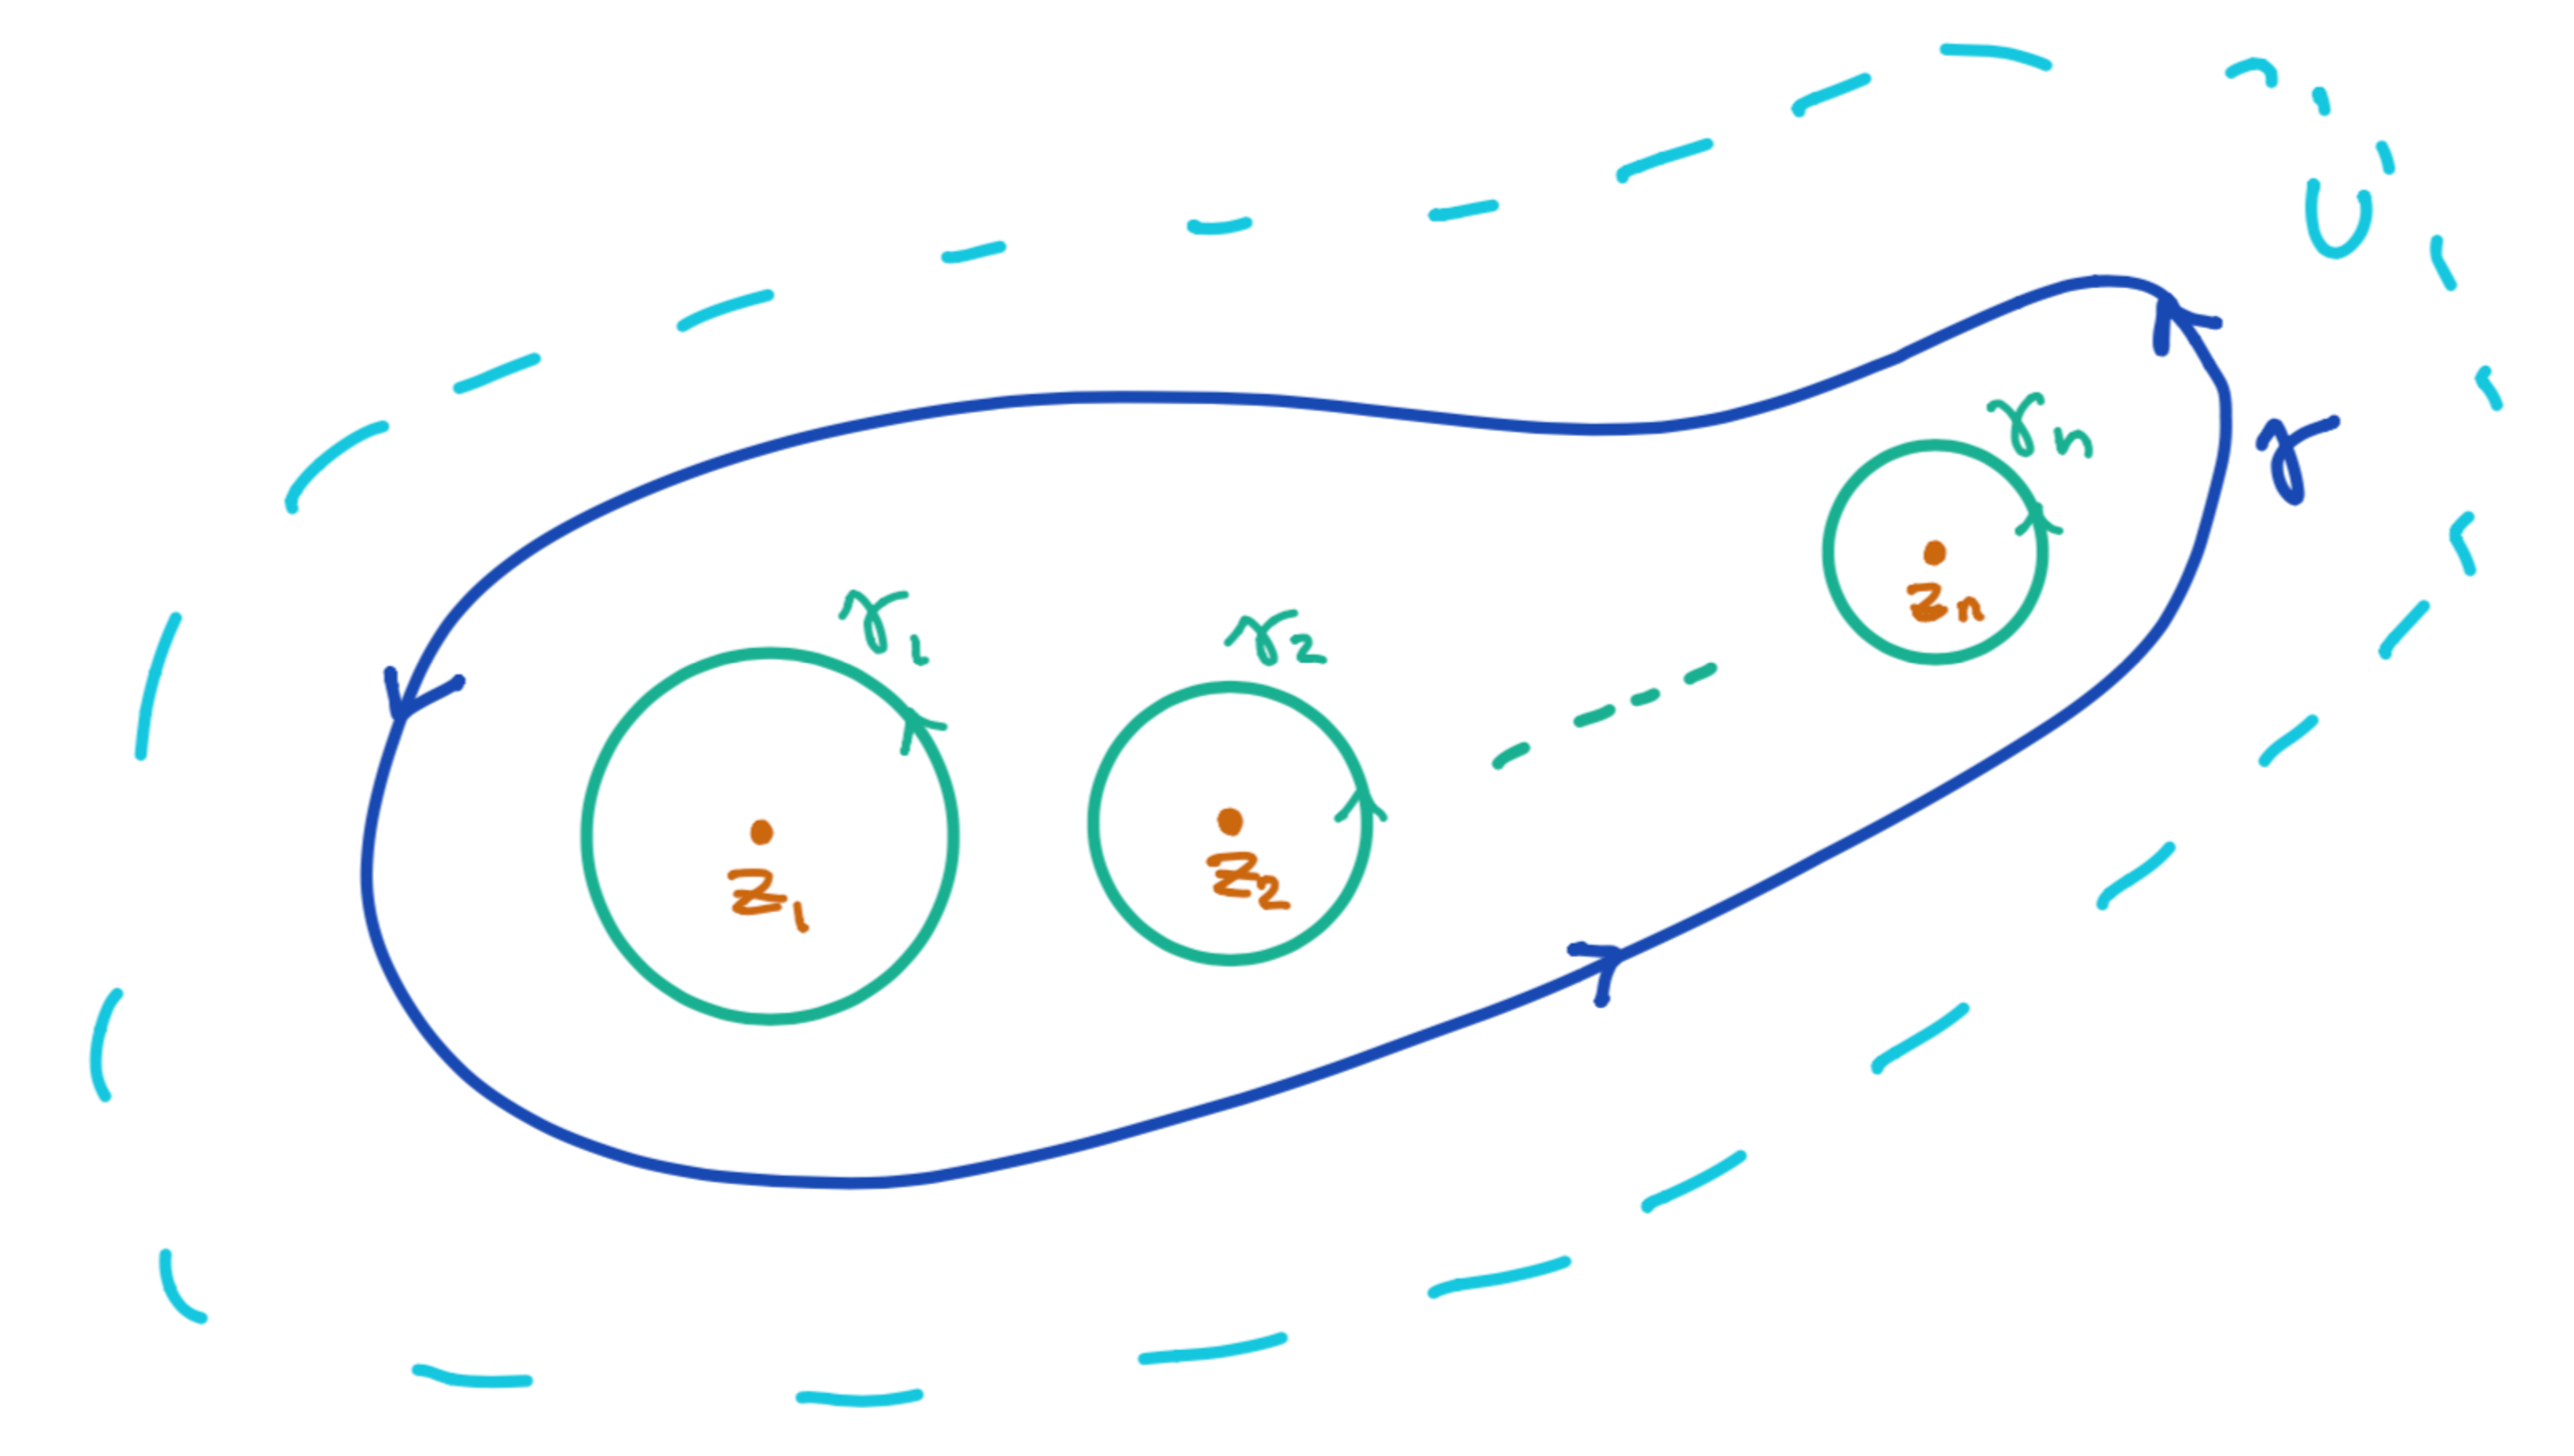
\includegraphics[width=0.9\linewidth]{assets/4-2-1.png}
  \caption{Kurven im Residuensatz}
\end{figure}

Dies lässt sich verallgemeinern für den Fall dass $\gamma$ kein einfacher oder positiv orientierter Pfad ist. Für einen beliebiegen geschlossenen Pfad $\gamma$ definieren wir die Windungszahl:

\begin{subbox}{Windungszahl}
  Die Windungszahl \(\operatorname{W}(\gamma,z)\) einer Kurve \(\gamma\) um einen Punkt \(z\) beschreibt wie oft sich \(\gamma\) um \(z\) im Gegenuhrzeigersinn dreht. Also: 
  \begin{itemize}
    \item \(\operatorname{W}(\gamma,z) = 1\) falls $\gamma$ sich um $z$ einmal im Gegenuhrzeigersinn (mathematisch positive Richtung) dreht
    \item \(\operatorname{W}(\gamma,z) = -1\) falls $\gamma$ sich um $z$ einmal im Uhrzeigersinn dreht
    \item \(\operatorname{W}(\gamma,z) = 0\) falls $z$ ausserhalb der Menge liegt welche von $\gamma$ umschlossen wird 
  \end{itemize}
  Die Windungszahl kann auch z.B. $0.5$ sein falls wir den Kreis nur zur Hälfte ''umlaufen''.
\end{subbox}

\begin{figure}[H]
  \centering 
  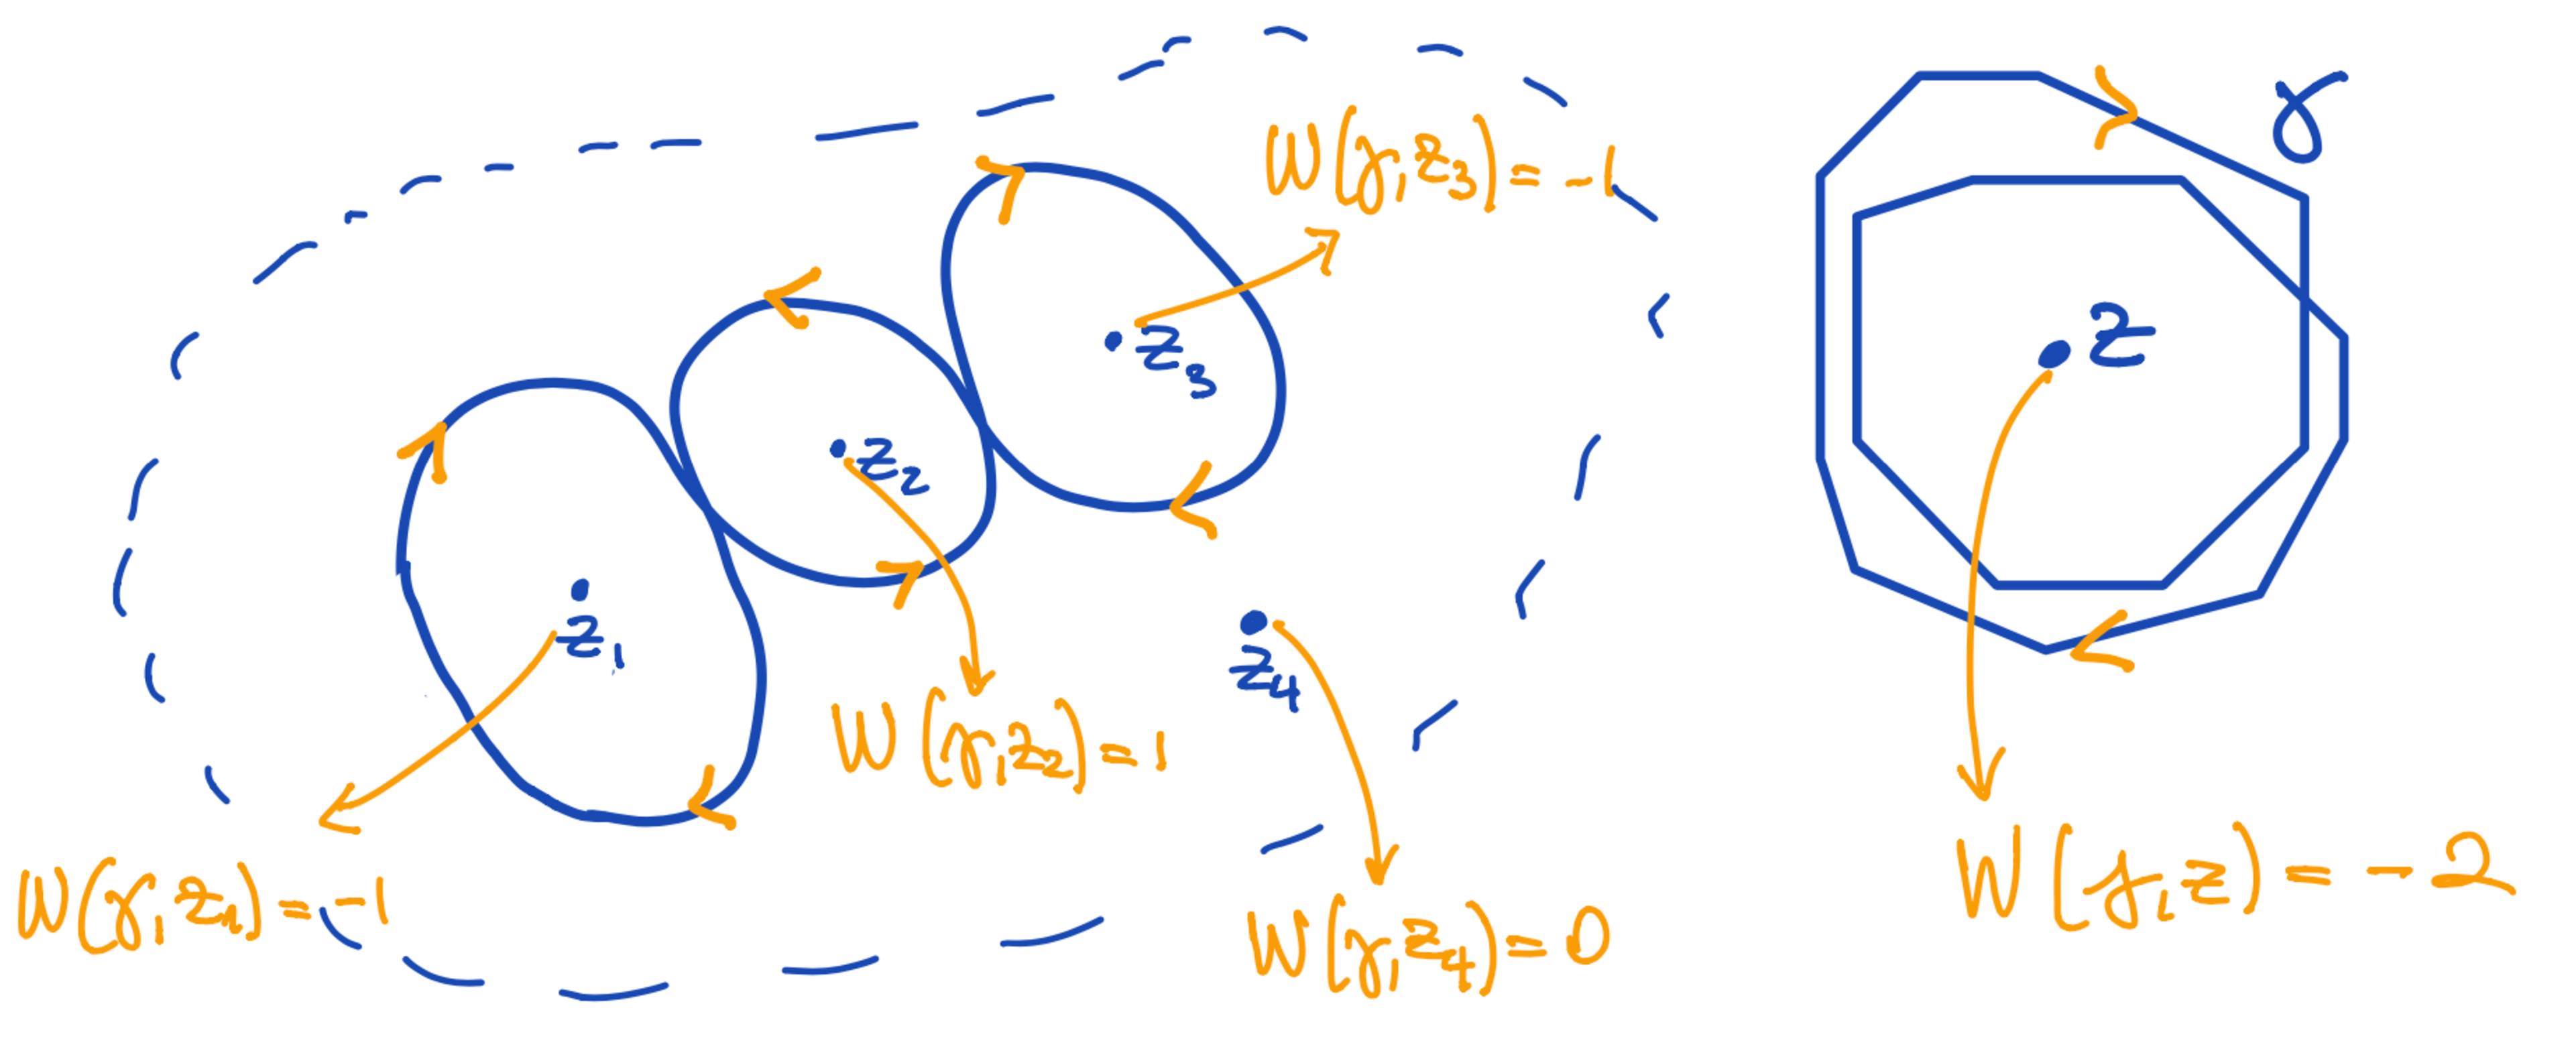
\includegraphics[width=0.9\linewidth]{assets/4-2-2.png}
  \caption{Windungszahl für verallgemeinerten Residuensatz}
\end{figure}

\begin{subbox}{Residuensatz (Verallgemeinerung)}
  Sei \(U\subset\mathbb{C}\) eine offene wegzusammenhängende Menge, \(\gamma\subset U\) eine Kurve und \(z_1,\dots,z_N\in U\). Sei \(f\colon U\setminus\{z_1,\dots,z_N\}\to \mathbb{C}\) holomorph. Dann gilt: \begin{align*} \int_{\gamma} f(z)dz = 2\pi i \sum_{k=1}^N \operatorname{W}(\gamma ,z_k) \cdot \operatorname{Res}(f,z_k) \end{align*}
\end{subbox}

\subsubsection{Berechnung von Residuen}

Für eine \textbf{hebbare Singularität} oder eine \textbf{Nullstelle} $z_0$ einer Funktion $f$ gilt in jedem Fall $c_n = 0$ für alle $n < 0$. Folglich gilt also auch $\Res(f, z_0) = c_{-1} = 0$.

Für \textbf{Polstellen} gibt es einige Lemmas:

\begin{subbox}{Residuen an Polstellen}
  Sei \(z_0\) eine isolierte Singularität der Funktion \(f\). Die Stelle \(z_0\) ist ein Pol der Ordnung \(m\geq1\) genau dann, wenn es eine Funktion $\phi$, welche an der Stelle \(z_0\) holomorph ist, gibt, mit \begin{align*} f(z)=\frac{\phi(z)}{(z-z_0)^m} \end{align*} wobei \(\phi(z_0)\neq0\) gilt. Falls $\phi(z_0) = 0$ muss man andere Methoden verwenden, z.B. die Laurentreihe entwickeln.
\end{subbox}

\begin{subbox}{Hebbare Singularität}
  $f$ hat eine hebbare Singularität an $z_0$, wenn $\lim_{z \to z_0} f(z)$ existiert. In diesem Falle gilt $\Res(f, z_0) = 0$.
\end{subbox}

Falls $\lim_{z \to z_0} |f(z)| = \infty$, so hat $f$ einen Pol an $z_0$.

\begin{subbox}{Polstellen}
  Sei $z_0$ ein Pol von $f$. Dann ist $z_0$ ein Pol $m$-ter Ordnung, wenn:
  $$
    \lim_{z \to z_0} (z - z_0)^m f(z) = a \neq 0
  $$
  wobei $a \in \C$.
\end{subbox}

\begin{mainbox}{Berechnung des Residuums an Polstellen}
  Falls \(z_0\) ein Pol der Ordnung \(m\) der Funktion \(f\) ist, gilt: \begin{align*} 
     \operatorname{Res}(f,z_0)= \lim_{z \to z_0} \frac{\phi^{(m-1)}(z)}{(m-1)!} 
  \end{align*}
  beziehungsweise:
  \begin{align*} 
    \operatorname{Res}(f,z_0)= \frac{\phi^{(m-1)}(z_0)}{(m-1)!} 
 \end{align*}
 falls $\phi^{m-1}$ in $z_0$ wohldefiniert ist.

 Wir können dies auch schreiben als:

$$
  \Res(f, z_0) = \frac{1}{(m - 1)!} \lim_{z \to z_0} \left( \frac{d^{m-1}}{dz^{m-1}} (z - z_0)^m f(z) \right)
$$
\end{mainbox}

Dies zeigen wir wie folgt: Nach Annahme schreben wir $f$ als:

$$
  f(z) = \frac{c_{-m}}{(z - z_0)^m} + \ldots + \frac{c_{-1}}{z - z_0} + c_0 + \ldots
$$
Folglich:
$$
  (z - z_0)^m f(z) = c_{-m} + \ldots + c_{-1} (z - z_0)^{m-1} + c_0 (z - z_0)^m + \ldots
$$
Nun gilt:
$$
\frac{d^{m-1}}{dz^{m-1}} (z - z_0)^m f(z) = (m - 1)! c_{-1} + (z - z_0) (c_0 + \ldots)
$$

Des Weiteren bemerken wir auch dass für $m = 1$ gilt dass $\Res(f, z_0) = \phi(z_0)$.

Ausserdem folgt auch dass falls $f$ einen Pol $z_0$ der Ordnung $m \geq 1$ hat, dass dann $\lim_{z \to z_0} f(z) = \lim_{z \to z_0} \frac{\phi(z)}{(z - z_0)^m}$ divergiert (da $\phi(z) \neq 0$).

\begin{mainbox}{Residuum bei einfachen Polen}
  Falls $z_0$ ein einfacher Pol der Funktion $f$ ist, gilt:
  $$
    \Res(f, z_0) = \lim_{z \to z_0} (z - z_0) f(z)
  $$
\end{mainbox}

\begin{mainbox}{Residuum für Pole bei Bruch}
  Sei $f(z) = \frac{p(z)}{q(z)}$ wobei $p$ und $q$ holomorph sind mit $p(z_0) \neq 0$ sowie $q(z_0) = 0$ und $q'(z_0) \neq 0$. Dann gilt:
  $$
    \Res(f, z_0) = \frac{p(z_0)}{q'(z_0)}
  $$
\end{mainbox}

Bei \textbf{wesentlichen Singularitäten} empfiehlt es sich die Laurentreihe zuerst zu berechnen. 

\begin{subbox}{Nullstellen}
  Sei $f: U \mapsto \C$ holomorph an der Stelle $z_0 \in U$. Die Funktion $f$ hat an der Stelle ein Nullstelle der Ordnung $m$ genau dann wenn es ein holomorphes $g: U \mapsto \C$ gibt mit $f(z) = (z - z_0)^m g(z)$ und $g(z_0) \neq 0$. 
\end{subbox}

Sind also $p,q$ holomorph an $z_0$ mit $p(z_0) \neq 0$ wobei $z_0$ eine Nullstelle der Ordnung $m$ für $q$ ist, dann gilt dass $z_0$ ein Pol der Ordnung $m$ für $\frac{p(z)}{q(z)}$ ist.

\begin{subbox}{}
  Sei $U \subset \C$ offen, $z_0 \in U$ und $f: U \setminus \{z_0\} \mapsto \C$ eine holomorphe Funktion. Angenommen $f(\overbar{z}) = \overbar{f(z)}$ für alle $z \in \C$. Dann gilt:
  $$
    \Res(f, \overbar{z_0}) = \overbar{\Res(f, z_0)}
  $$
\end{subbox}

\subsection{Bedingungen, unter denen $f(z) \equiv 0$}

\begin{mainbox}{Isolierte Nullstellen}
  Sei \(f\colon B(z_0,\epsilon)\to\mathbb{C}\) holomorph und sei \(f(z_0)=0\). Entweder ist \(f(z) = 0\) für alle \(z \in B(z_0,\epsilon)\) oder \(z_0\) ist eine isolierte Nullstelle von \(f\).
\end{mainbox}

\begin{subbox}{Nullfunktion}
  Sei \(f\colon U\to \mathbb{C}\) holomorph und \(U\) wegzusammenhängend. Falls \(f(z)\equiv0\) auf einer offenen Menge oder auf einer geraden Strecke, dann ist \(f\equiv0\) auf ganz \(U\).
\end{subbox}

\begin{mainbox}{Identitätsprinzip für holomorphe Funktionen}
  Seien \(U\subseteq \mathbb{C}\) offen, \(f,g \colon U \to \mathbb{C}\) holomorph. Falls \(f(z) = g(z)\) auf einer offenen Menge oder auf einer geraden Strecke in \(U\), dann gilt auf ganz $U$: \begin{align*}f(z)\equiv g(z)\end{align*}
\end{mainbox}

Holomorphe Funktionen sind also \textbf{eindeutig definiert wenn man} sie in einer \textbf{Teilmenge kennt}.

Daraus folgern wir z.B. dass $f(z) := \sin^2(z) + \cos^2(z) - 1 \equiv 0$ für jedes $z \in \C$, denn es gilt $f(x) = 0$ für jedes $x \in \R$.

\subsection{Anwendungen des Residuensatzes auf reelle Integrale}

\begin{subbox}{Cauchy-Hauptwert}
  Der Limes \begin{align*} \lim_{R\to\infty}\int_{-R}^Rf(z)\,dz \end{align*} wird als Cauchy-Hauptwert (principal value) des Integrals \(\int_{-\infty}^\infty f(z)\,dz\) bezeichnet \begin{align*} P.V.\int_{-\infty}^\infty f(z)\,dz=\lim_{R\to\infty}\int_{-R}^Rf(z)\,dz \end{align*}
\end{subbox}

\begin{subbox}{Uneigentliches Integral}
  Die Definition vom uneigentlichen Integral lautet \begin{align*} \int_{-\infty}^\infty f(x)\,dx=\lim_{R\to\infty}\int_{-R}^0f(x)\,dx+\lim_{R\to\infty}\int_{0}^Rf(x)\,dx \end{align*} falls beide Integrale an der rechten Seite existieren. Falls beide Integrale auf der rechten Seite existieren, existiert auch \(\lim_{R\to\infty}\int_{-R}^Rf(x)\,dx\). Die Umkehrung dieser Aussage ist aber nicht wahr, wie das Beispiel von \(f(x)=x\) zeigt.
\end{subbox}

Wir versuchen nun Integrale der Form $\int_{-\infty}^\infty f(x) \dx$ mit dem Residuensatz zu berechnen.

\begin{figure}[H]
  \centering 
  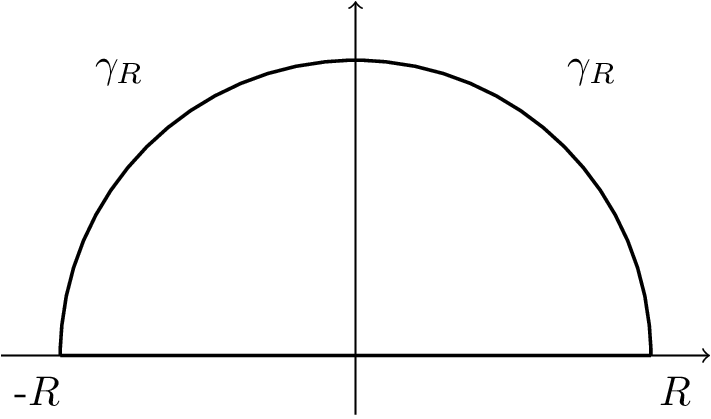
\includegraphics[width=0.5\linewidth]{assets/4-4-1.png}
  \caption{Kurve zur Berechnung des uneigentlichen Integrals}
\end{figure}

Wir betrachten den Pfad $\gamma_R$, d.h. den Halbkreis mit Radius $R$ im ersten und zweiten Quadranten, im Gegenuhrzeigersinn orientiert.

Die Kurve \(\gamma_R\ast[-R,R]\) ist eine geschlossene Kurve und wir können deshalb den Residuensatz anwenden, um das Integral zu berechnen. Daraus folgt, dass 
\begin{align*} \int_{\gamma_R\ast[-R,R]} f(x) dx=2\pi i\sum_{j=1}^{n_R}\operatorname{Res}(f,z_j)\,, \end{align*} 
wobei \(z_1,\dots, z_{n_R}\) die Pole innerhalb der Kurve \(\gamma_R\ast[-R,R]\) sind.


Aus (KI3) auf der linken Seite angewendet erhalten wir \begin{align*} \int_{\gamma_R} f(x) dx+\int_{-R}^{R} f(x) dx=2\pi i\sum_{j=1}^{n_R}\operatorname{Res}(f,z_j) \end{align*} Wir nehmen jetzt den Limes für \(R \to \infty\). Falls \begin{align*} \lim_{R\to \infty} \int_{\gamma_R} f(z)dz = 0  \end{align*} erhalten wir \begin{align*} \lim_{R\to\infty}\int_{-R}^Rf(z)\,dz=2\pi i\sum_{j=1}^{n}\operatorname{Res}(f,z_j) \end{align*} wobei die Summe jetzt über alle Pole \(z_1,\dots, z_n\) mit \(\Im(z_j)>0\), \(j=1,\dots,n\) geht.

Nachfolgend geben wir jetzt eine Bedingung dafür dass das obige Integral über $\gamma_R$ verschwindet.

\begin{subbox}{Uneigentliches Integral mit Residuensatz}
  Sei \(\gamma_R(t):=Re^{ i t}\) für \(t\in[0,\pi]\). Seien \(p\) und \(q\) Polynome mit den folgenden Eigenschaften:
  \begin{itemize}
    \item \(\deg(p)\leq \deg(q)-2\)
    \item \(q(x)\) besitzt keine Nullstellen auf der \(x\)-Achse
  \end{itemize}


Sei: \begin{align*} f(z) := \frac{p(z)}{q(z)}h(z)\,. \end{align*} wobei \(|h(z)|\) auf der Menge \(\{z\in\mathbb{C}:\,\Im(z)\geq0\}\) beschränkt ist. Dann gilt: \begin{align*} \lim_{R\to \infty} \int_{\gamma_R} f(z)\,dz = 0 \end{align*}

Somit gilt auch:

\begin{align*} P.V.\int_{-\infty}^\infty f(x) dx = 2 \pi i \sum_{z_j}\operatorname{Res} \left( \frac{p(z)}{q(z)}h(z),z_j \right) \end{align*} wobei \(z_j\) die Pole sind, welche in der Menge \(\{z\in\mathbb{C}:\,\Im(z)>0\}\) enthalten sind.

\end{subbox}

Bestimmen wir z.B. folgendes Integral: \begin{align*} \int_{-\infty}^{\infty} \frac{1}{(1+x^2)^2}dx\end{align*}

In diesem Fall sind \(p(z)=1\), \(q(z) = (1+z^2)^2\) mit \(q(x) > 0\) für jedes \(x\in\mathbb{R}\), und \(h(z)=1\). Hier ist die Funktion \(f(z)\) gerade und dann ist \begin{align*} \int_{-\infty}^\infty \frac{1}{(1+x^2)^2}\,dx =2 \pi i \sum_{z_j}\operatorname{Res} \left(\frac{1}{(1+z^2)^2},z_j \right) \end{align*}

Die Pole vom Integrand sind deshalb die Nullstellen von \(q\), d.h. \(z_{\pm}= \pm i\) und \(z_-= i\) ist der einzige Pol, der innerhalb von \(\gamma_R\ast[-R,R]\) mit \(\gamma_R(t):=Re^{ i t}\), für \(t\in[0,\pi]\) enthalten ist. Ausserdem ist \(z_-= i\) ein Pol der Ordnung 2. Um \(\operatorname{Res} \left(\frac{1}{(1+z^2)^2}, i \right)\) zu berechnen schreiben wir \begin{align*} f(z)=\frac{1}{(1+z^2)^2}=\frac{\phi(z)}{(z- i)^2}\,, \end{align*} wobei \(\phi(z)=\frac{1}{(z+ i)^2}\), mit \(\phi\) holomorph um \(z= i\) und \(\phi( i)\neq0\). Nun gilt: \begin{align*} \operatorname{Res}(f, i) = \frac{\phi'( i)}{1!} = -\frac{2}{( i + i)^3} = \frac{-2}{-8 i} = \frac{- i}{4}\,. \end{align*} Also: \begin{align*} \int_{-\infty}^\infty \frac{1}{(1+x^2)^2}\,dx =2\pi i\operatorname{Res} \left(\frac{1}{(1+x^2)^2}, i \right)= 2\pi i\frac{- i}{4}=\frac{\pi}{2}\,□ \end{align*}

Falls $q$ nun aber eine Nullstelle auf der $x$-Achse hat, müssen wir anders vorgehen.

\begin{figure}[H]
  \centering 
  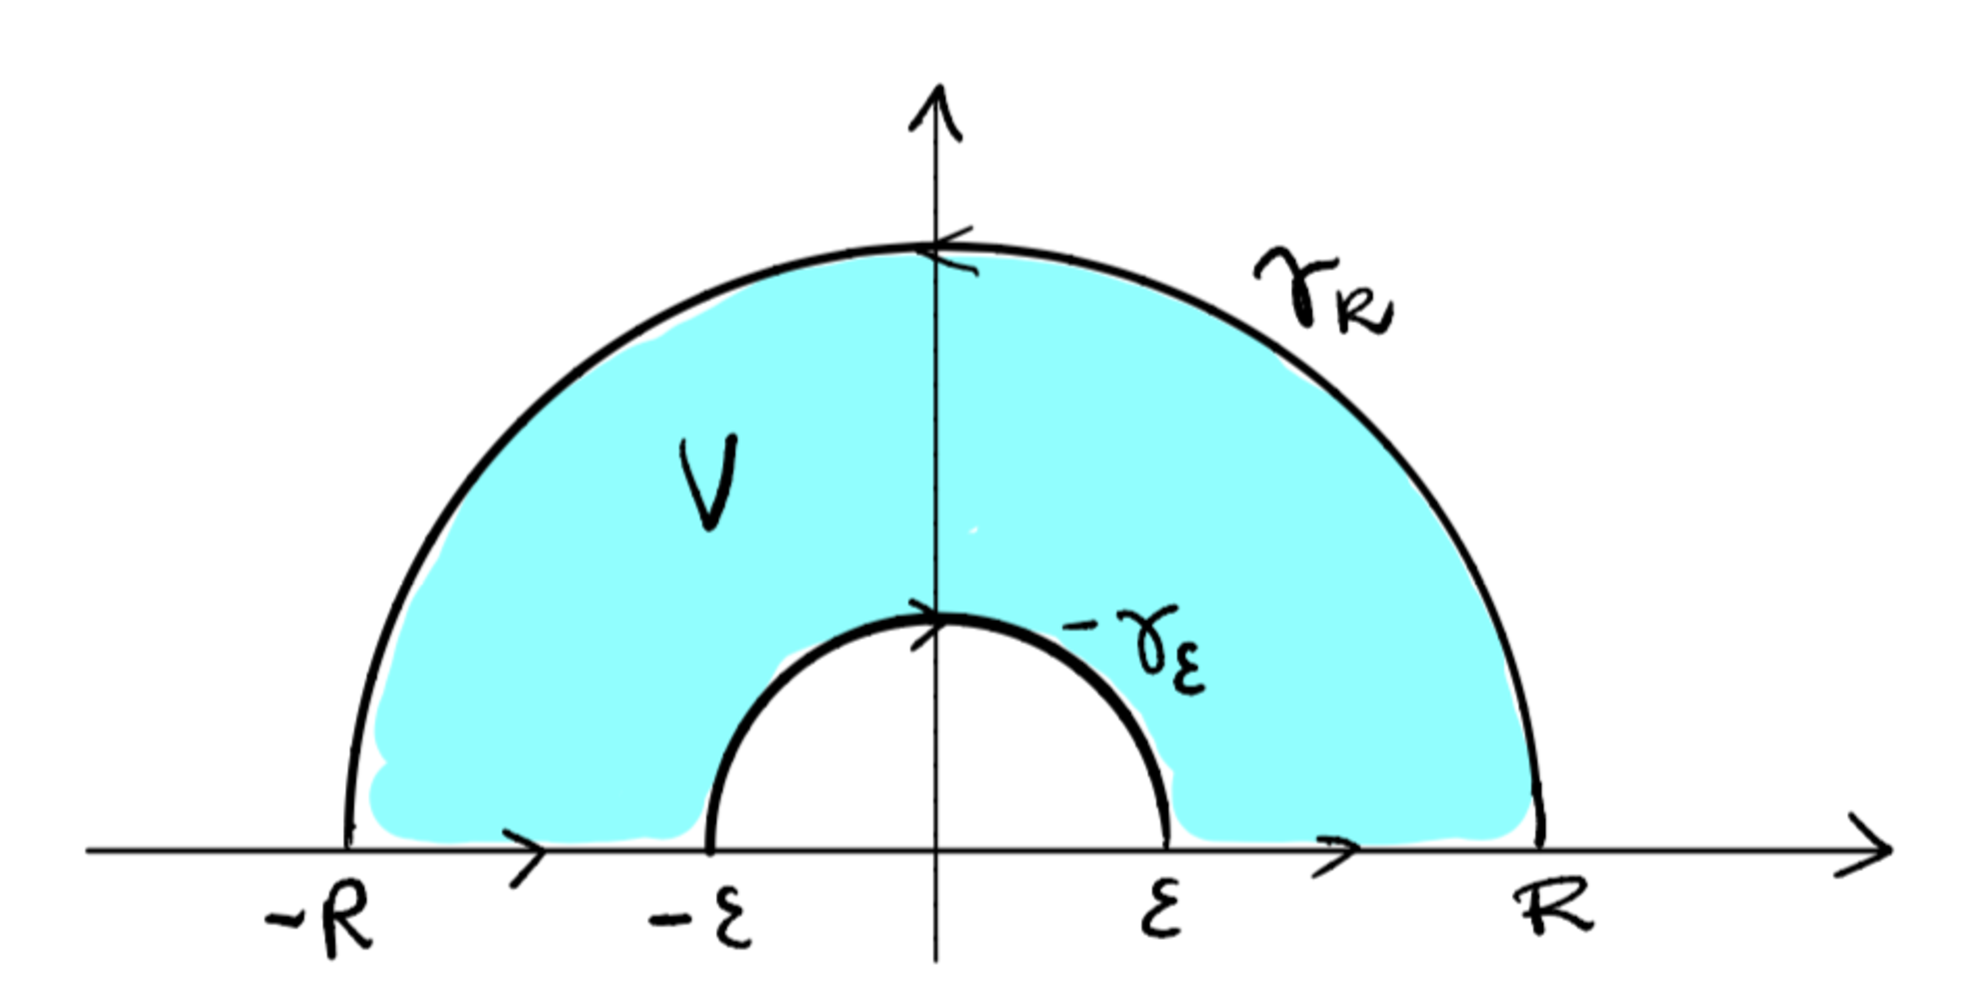
\includegraphics[width=0.75\linewidth]{assets/4-4-2.png}
  \caption{Parameterisierung falls $q$ Nullstellen auf der $x$-Achse hat}
\end{figure}

Sei $V$ das obige Gebiet wobei wir mit $\partial V$ den Rand bezeichnen. Da $f$ auf $V$ holomorph ist gilt wegen dem Satz von Cauchy:

\begin{align*} \int_{\partial V}f(z)\,dz=0 \end{align*} 

Nun gilt aber auch:
\begin{align*} \int_{\partial V}f(z)\,dz=\int_{\gamma_R} f(z)\,dz+\int_{-R}^{-\epsilon}f(z)\,dz+\int_{-\gamma_\epsilon} f(z)\,dz+\int_\epsilon ^Rf(z)\,dz \end{align*}

Schlussendlich:
\begin{align*} \int_{-\infty}^\infty f(z)dz= -\lim_{R\to\infty}\int_{\gamma_R}f(z)\,dz -\lim_{\epsilon\to0}\int_{-\gamma_\epsilon} f(z)dz  \end{align*}

Beim Integral über die Kurve $-\gamma_{\epsilon}$ ist zu beachten dass die Windungszahl $-0.5$ ist.

\begin{subbox}{Residuensatz mit Halbkreis}
  Sei \(f\) eine holomorphe Funktion auf \(B(x_0,R)\setminus\{x_0\}\), wobei \(x_0\in\mathbb{R}\) und \(R>0\). Nehmen wir an, dass \(x_0\) ein einfacher Pol von \(f\) ist. Sei \(\gamma_\epsilon\) ein im Gegenuhrzeigersinn durchlaufenen Halbkreis um \(x_0\) mit \(\Im(\gamma_\epsilon)>0\) und \(\epsilon< R\). Dann:
  \begin{align*} \lim_{\epsilon \to 0} \int_{\gamma_{\epsilon}} f(z) dz = \pi i \operatorname{Res}(f,x_0) \end{align*}

\end{subbox}

\begin{figure}[H]
  \centering 
  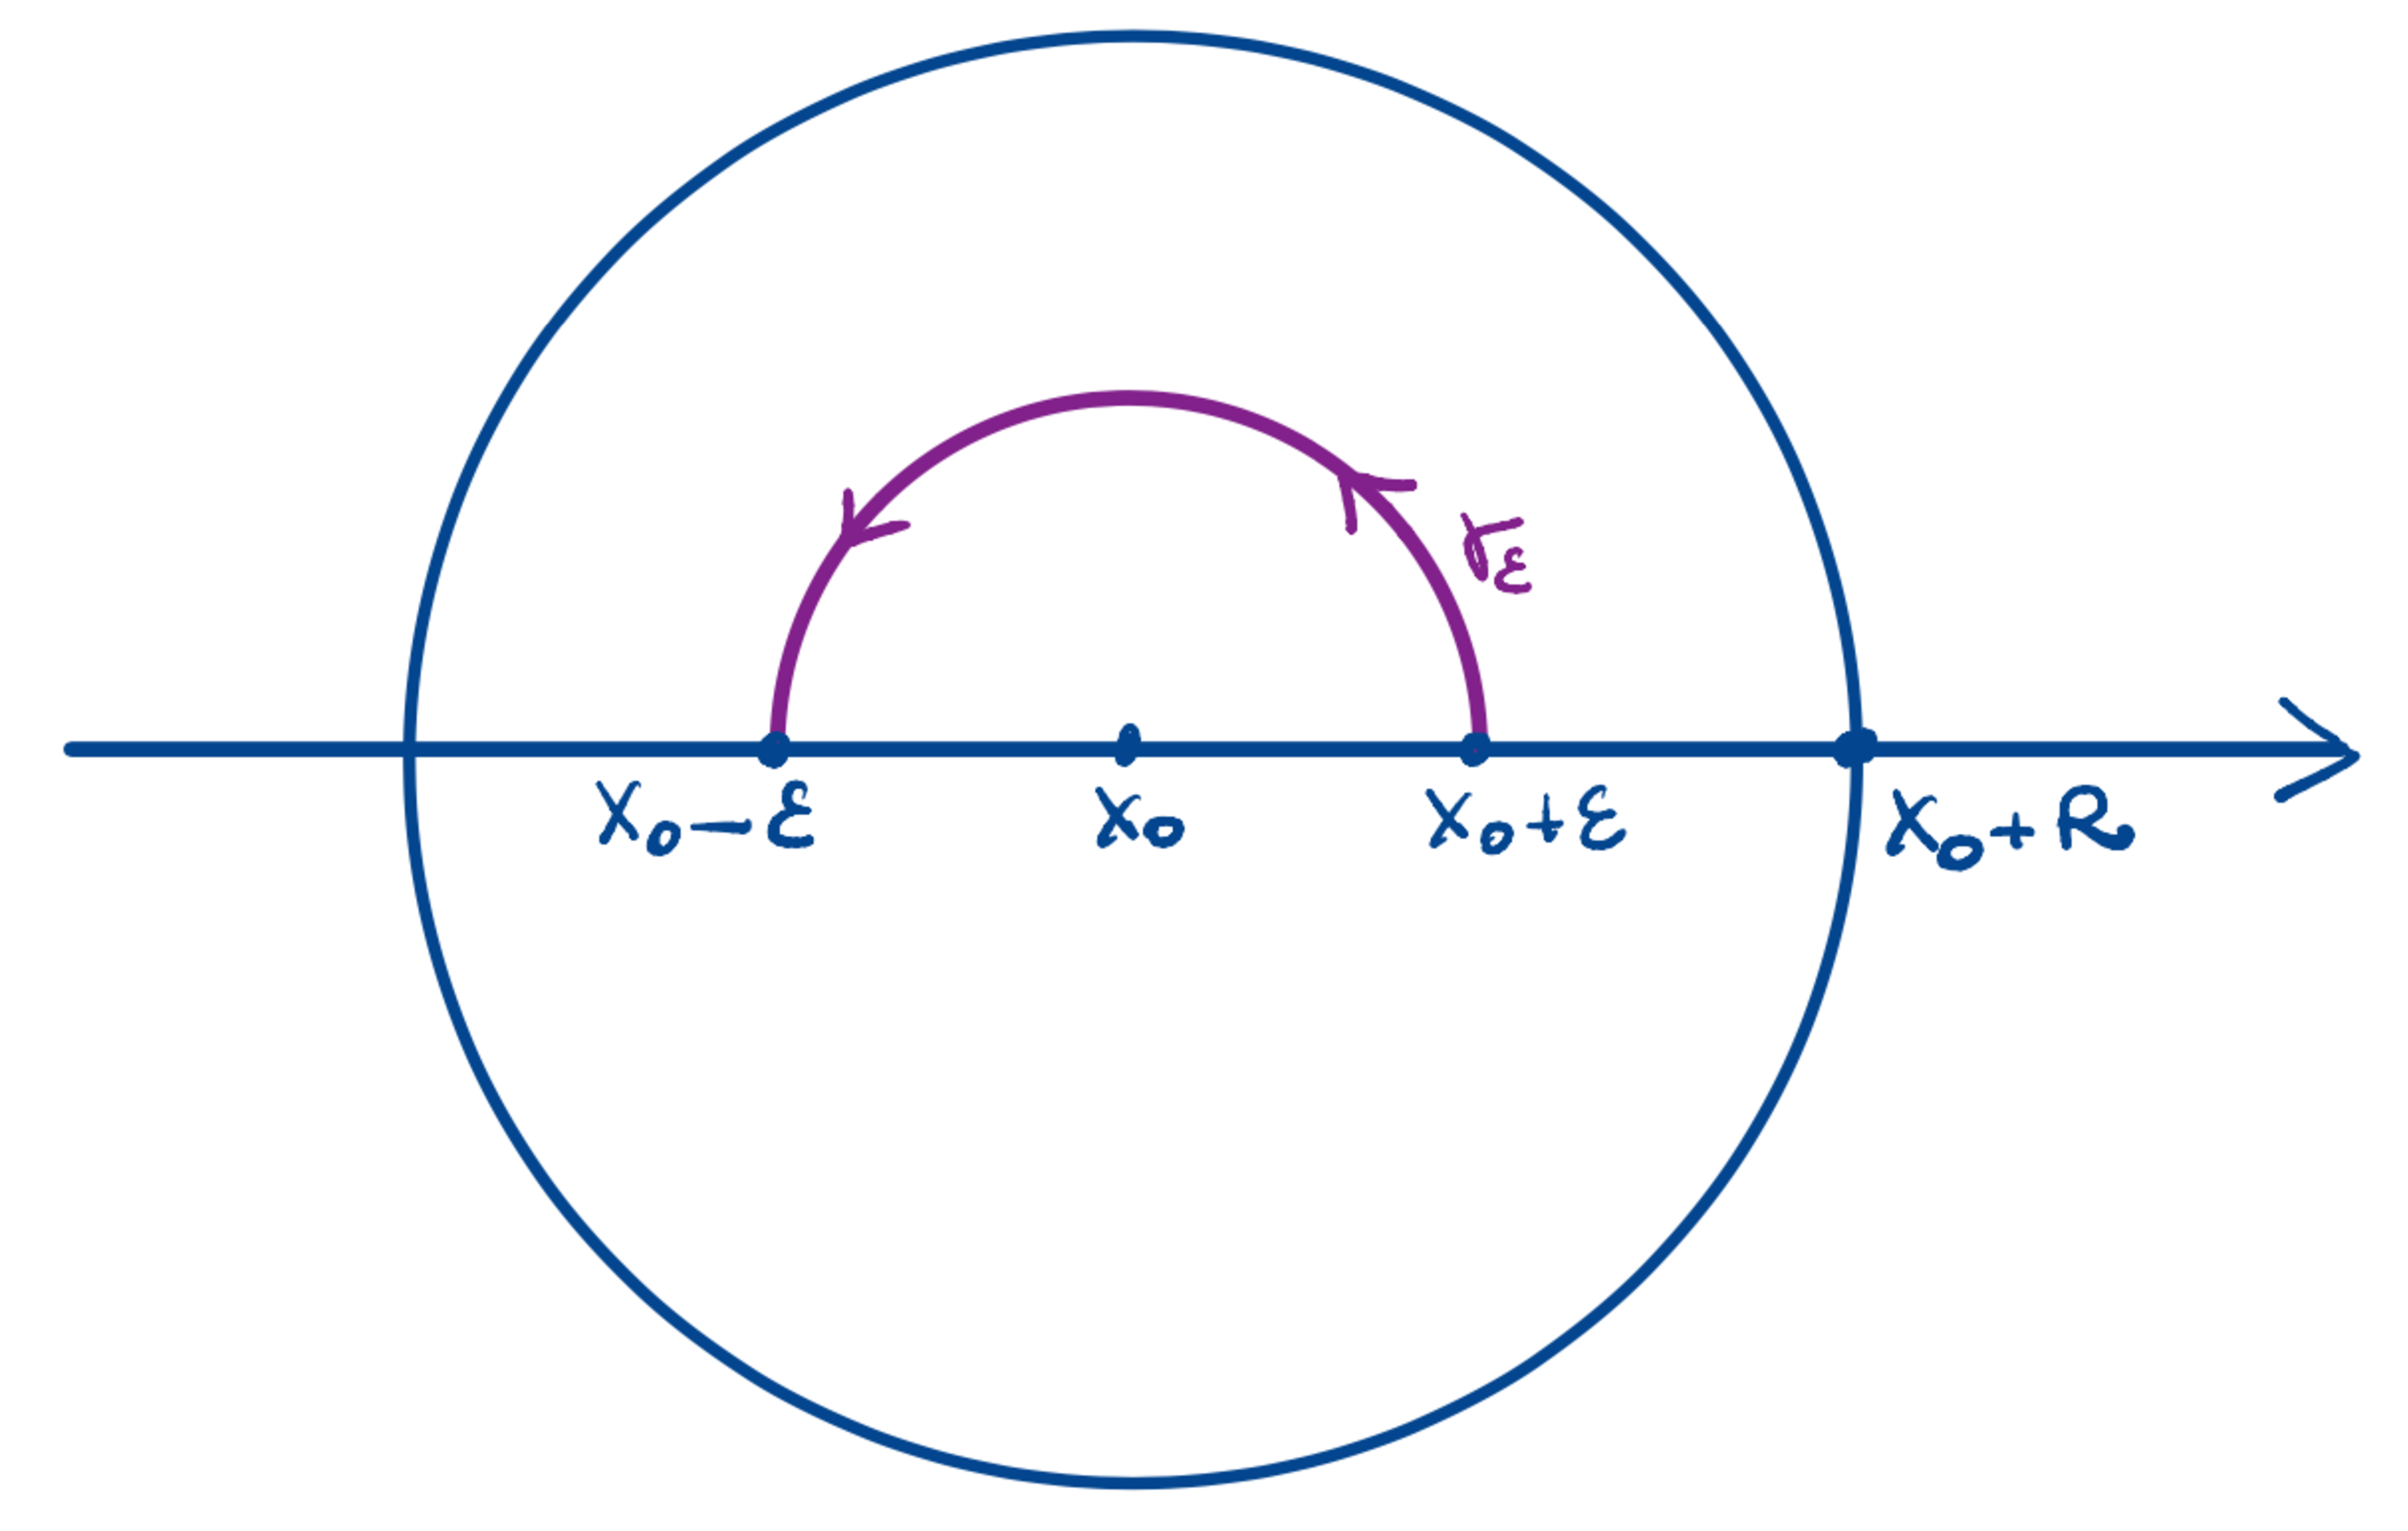
\includegraphics[width=0.5\linewidth]{assets/4-4-3.png}
  \caption{Residuensatz mit Halbkreis}
\end{figure}

\subsection{Uneigentliche reelle Integrale}
	
Falls \( f(z) = \dfrac{p(z)}{q(z)} \) und \( q(z) \neq 0\)  \(\forall z \in \mathbb{R}\) und \( \deg(p) \leqslant \deg(q) - 2 \) wie zuvor:

  \[ \displaystyle \int\limits_{-\infty}^\infty f(x) e^{i\alpha x}dx = \begin{cases}
  \displaystyle 2\pi i \sum\limits_{z_i \in H^+} \Res\big(f(z)e^{i\alpha z}, z_i\big)	&	\alpha \geqslant 0\\
  \displaystyle -2\pi i \sum_{z_i \in H^-} \Res\big(f(z)e^{i\alpha z}, z_i\big)		&	\alpha \leqslant 0\\
\end{cases} \]
  \[ \displaystyle \int\limits_{-\infty}^\infty f(x) \cos(\alpha x)dx = \begin{cases}
    
  \displaystyle -2\pi\cdot \text{Im}\left(\sum_{z_i \in H^+} \Res\big(f(z)e^{i\alpha z},  z_i\big) \right)
  &	\alpha \geqslant 0\\
  \displaystyle 2\pi\cdot \text{Im}\left(\sum_{z_i \in H^-} \Res\big(f(z)e^{i\alpha z},  z_i\big) \right)
  &	\alpha \leqslant 0\\
\end{cases} \]

  \[ \displaystyle \int\limits_{-\infty}^\infty f(x) \sin(\alpha x)dx = \begin{cases}
  \displaystyle 2\pi\cdot \text{Re}\left(\sum_{z_i \in H^+} \Res\big(f(z)e^{i\alpha z},  z_i\big) \right)
  &	\alpha \geqslant 0\\
  \displaystyle -2\pi\cdot \text{Re}\left(\sum_{z_i \in H^-} \Res\big(f(z)e^{i\alpha z},  z_i\big) \right)
  &	\alpha \leqslant 0\\
\end{cases} \]

$H^+$ ist die obere Halbebene, $H^-$ die untere Halbebene. In den unteren Halbebene wird der Pfad im Uhrzeigersinn parametrisiert, folglich haben wir ein negatives Vorzeichen.

\section{Fourier-Analysis}

\subsection{Fourier-Reihen}

\begin{subbox}{Periode und Fundamentalperiode}
  Sei \(f\colon\mathbb{R}\to\mathbb{C}\). Falls es \(p\in\mathbb{R}\) gibt, so dass \begin{align*}f(t+p)=f(t)\text{ für jedes }t\in\mathbb{R}\end{align*} heisst \(f\) periodisch und \(p\) heisst die Periode von \(f\). Die Frequenz von \(f\) ist $f=\frac{1}{p}$. Die kleinste Periode (falls sie existiert) heisst die Fundamentalperiode.
\end{subbox}

$f(t) = c$ mit $c \in \C$ ist auch periodisch, aber hat keine Fundamentalperiode.

Die Summe periodischer Funktionen ist immer dann periodisch, wenn die Perioden aller Summanden ein gemeinsames Vielfaches haben. In diesem Fall ist die Periode das (kleinste) gemeinsame Vielfache. Gleichermassen für das Produkt aus periodischen Funktionen.

\begin{subbox}{Integral periodischer Funktionen}
  Sei $f: \R \mapsto \C$ eine stetige $L$-periodische Funktion. Für ein beliebiges $\alpha \in \R$ gilt:
  $$
    \int_{0}^L f(t) dt = \int_{\alpha}^{\alpha + L} f(t) dt
  $$
\end{subbox}

\begin{subbox}{Trigonometrisches Polynom}
  Ein trigonometrisches Polynom N-ten Grades ist eine endliche Linearkombination
   \begin{align*} \frac{a_0}{2}+\sum_{n=1}^N\left(a_n\cos\left(\frac{n\pi}{L}t\right)+b_n\sin\left(\frac{n\pi}{L}t\right)\right) \end{align*}
   von Funktionen in der Menge
    \begin{align*} \left\{\sin\left(\frac{n\pi}{L}t\right),\cos\left(\frac{n\pi}{L}t\right): n\in\mathbb{Z}, n\geq0\right\} \end{align*}
    wobei \(a_N\neq0\) oder \(b_N\neq0\), oder, äquivalent, eine endliche Linearkombination \begin{align*} \sum_{n=-N}^Nc_ne^{ i\frac{n\pi}{L}t} \end{align*}
     von Funktionen in der Menge \begin{align*} \left\{e^{ i\frac{n\pi}{L}t}:\,n\in\mathbb{Z}\right\} \end{align*} wobei \(c_N\neq0\). Eine formelle Reihe \begin{align*} \frac{a_0}{2}+\sum_{n=1}^\infty\left(a_n\cos\left(\frac{n\pi}{L}t\right)+b_n\sin\left(\frac{n\pi}{L}t\right)\right) \end{align*} oder \begin{align*} \sum_{n=-\infty}^\infty c_ne^{ i\frac{n\pi}{L}t} \end{align*} heisst eine trigonometrische Reihe.
 
\end{subbox}

\begin{subbox}{Orthonormalitätsbeziehungen für $e^{i\frac{n\pi}{L}t}$}
  Seien \(n,m\in\mathbb{Z}\). Dann gilt: \begin{align*} \frac{1}{2L}\int_{-L}^L e^{ i \frac{n\pi}{L}t}e^{- i \frac{m\pi}{L}t}\,dt =\begin{cases} 1&n=m\\ 0&n\neq m \end{cases} \end{align*}
\end{subbox}

\begin{subbox}{Orthonormalitätsbez. für $\cos(\frac{n\pi}{L}t)$ und $\sin(\frac{n\pi}{L}t)$}
  Seien \(n,m\in\mathbb{N}\cup\{0\}\). Dann gilt:
\begin{align*}\int_{-L}^L\cos\left(\frac{n\pi}{L}t\right)\cos\left(\frac{m\pi}{L}t\right)\,dt=\begin{cases}0&n\neq m\\L&n=m\neq0\\2L&n=m=0 \end{cases} \end{align*}
\begin{align*} \int_{-L}^L\sin\left(\frac{n\pi}{L}t\right)\sin\left(\frac{m\pi}{L}t\right)\,dt=\begin{cases}0&n\neq m \lor n = m = 0\\L&n=m\neq0 \end{cases} \end{align*}
\begin{align*} \int_{-L}^L\cos\left(\frac{n\pi}{L}t\right)\sin\left(\frac{m\pi}{L}t\right)\,dt=0, \text{ für jedes }n,m  \end{align*}

\end{subbox}

\begin{mainbox}{Fourierreihe}
  Sei \(f\) eine \(2L\)-Periodische Funktion, die durch eine trigonometrische Reihe \begin{align*} f(t)\sim \frac{a_0}{2}+\sum_{n=1}^\infty\left(a_n\cos\left(\frac{n\pi}{L}t\right)+b_n\sin\left(\frac{n\pi}{L}t\right)\right)  \end{align*} 
  oder 
  \begin{align*} f(t)\sim \sum_{n=-\infty}^\infty c_ne^{ i\frac{n\pi}{L}t} \end{align*} dargestellt werden kann. Dann gilt 
  \begin{align*} a_m=\frac{1}{L}\int_{-L}^Lf(t)\cos\left(\frac{m\pi}{L}t\right)\,dt \text{ falls } m\geq 0  \end{align*} \begin{align*} b_m=\frac{1}{L}\int_{-L}^Lf(t)\sin\left(\frac{m\pi}{L}t\right)\,dt \text{ falls } m>0  \end{align*} und \begin{align*} c_m=\frac{1}{2L}\int_{-L}^Lf(t)e^{- i \frac{m\pi}{L} t}\,dt \text{ falls } m\in\mathbb{Z}  \end{align*}

  Bei Funktionen mit periodischer Fortzsetzung ist bei der Berechnung der Koeffizienten darauf zu achten das Integral im richtigen Bereich zu evaluieren ($-L$ und $L$ entsprechend verschieben).

\end{mainbox}

Ist $f$ reellwertig, so sind auch alle $a_k$ und alle $b_k$ reell; ist $f$ gerade, so treten nur Cosinusterme auf, und ist $f$ ungerade, so treten nur Sinusterme auf.

$\frac{a_0}{2}$ ist der Mittelwert von $f$ auf einer Periode. $a_1\cos\left(\frac{\pi}{L}t\right)+b_1\sin\left(\frac{\pi}{L}t\right)$ ist die 1. Harmonische oder Grundschwingung. $a_n\cos\left(\frac{n\pi}{L}t\right)+b_n\sin\left(\frac{n\pi}{L}t\right)$ ist die $n$-te Harmonische oder $n-1$-te Oberschwingung.

\begin{mainbox}{Beziehungen zwischen Koeffizienten}
  Für die Koeffizienten der Fourierreihe gilt:
  \begin{align*} 
    c_n&=\frac{1}{2}(a_n- i b_n) & c_{-n} =\frac{1}{2}(a_n+ i b_n)\\ 
    a_n&=c_n+c_{-n} & b_n = i(c_n-c_{-n})  \end{align*}

\end{mainbox}

\begin{subbox}{Fourierreihe ungerader und gerader Funktionen}
  Sei \(f\) eine \(2L\)-periodische Funktion mit Fourier-Reihen Entwicklung.
  \begin{itemize}
    \item{
      Falls \(f\) gerade ist, sind alle \(b_n=0\) und \begin{align*} a_n&=\frac{2}{L}\int_0^Lf(t)\cos\left(\frac{n\pi}{L}t\right)\,dt\,,\text{ für }n\geq0 \end{align*}
    }
    \item{
      Falls \(f\) ungerade ist, sind alle \(a_n=0\) und \begin{align*} b_n=\frac{2}{L}\int_0^Lf(t)\sin\left(\frac{n\pi}{L}t\right)\,dt\,,\text{ für }n\geq1 \end{align*}
    }
  \end{itemize}

  Bei Funktionen mit periodischer Fortzsetzung ist bei der Berechnung der Koeffizienten darauf zu achten das Integral im richtigen Bereich zu evaluieren ($-L$ und $L$ entsprechend verschieben).
\end{subbox}

\begin{subbox}{Konvergenz von Fourierreihen}
  Sei \(f\) eine \(2L\)-periodische Funktion auf \([-L,L]\), die stückweise stetig ist und die eine linke und rechte Ableitung an jedem Punkt in \([-L,L]\) besitzt. Dann ist die Fourier-Reihen Entwicklung von \(f\) auf \([-L,L]\) konvergent. An jedem Punkt \(t\in[-L,L]\), wo \(f\) stetig ist, ist die Summe der Fourier-Reihe gleich \(f(t)\):
   \begin{align*} \frac{a_0}{2}+\sum_{k=1}^\infty\left(a_k\cos\left(\frac{n\pi}{L}t\right)+b_k\sin\left(\frac{n\pi}{L}t\right)\right)=f(t) \end{align*}
    und an einer Sprungstelle \(t_0\in[-L,L]\) gilt:
     \begin{align*} \frac{a_0}{2}+\sum_{k=1}^\infty\left(a_k\cos\left(\frac{n\pi}{L}t_0\right)+b_k\sin\left(\frac{n\pi}{L}t_0\right)\right)=\\\frac12\left(\lim_{t\to t_0^-}f(t)+\lim_{t\to t_0^+}f(t)\right) \end{align*}
\end{subbox}

\begin{subbox}{Eindeutigkeit der Fourierreihe}
  Sei \(f\) eine \(2\pi\)-periodische Funktion auf \([-L,L]\), die stückweise stetig ist und die die linke und rechte Ableitung an jedem Punkt in \([-L,L]\) hat. Dann besitzt \(F\) genau eine Fourier-Reihe, durch welche sie für alle \(f\in\mathbb{R}\) dargestellt wird.
\end{subbox}

Als Gibbs'sches Phänomen bezeichnet man das Verhalten, dass bei abgebrochenen Fourierreihen und bei der Fourier-Transformation von stückweise stetigen, differenzierbaren Funktionen in der Umgebung von Sprungstellen sogenannte Überschwingungen auftreten. Diese Überschwingungen verschwinden auch dann nicht, wenn die endliche Anzahl von Termen zur Approximierung bzw. die Bandbreite auf beliebig hohe, aber endliche Werte erhöht wird, sondern weisen in der maximalen Auslenkung eine konstante, relative Auslenkung von ca. 9\% auf.

Wir betonen, dass das Überschwingen nicht nach null geht, aber die Grenze der Folge von Teilsummen (das ist die Fourier-Reihe) kein Überschwingen hat. Darin besteht kein Widerspruch, da sich der Punkt, an dem das Überschwingen auftritt, in Richtung des Sprunges bewegt. Wir haben punktweise Konvergenz, aber keine gleichmässige Konvergenz.

\subsection{Fourier-Transformation}

Falls \(f\) eine \(2L\)-periodische Funktion ist, haben wir im letzen Kapitel ihre Fourier-Reihe studiert. Man kann die Fourier-Koeffizienten von \(f\) als eine Funktion \begin{align*} \begin{aligned} \hat f\colon\mathbb{Z}&\longrightarrow~~~\mathbb{C}\\ n&\mapsto \hat f( n ):=\langle f,\mathbf{e}_{n,L}\rangle=c_n \end{aligned} \end{align*} auffassen. Die Funktion \(\hat f\) wird die Fourier-Transformation von \(f\) genannt. Wir betrachten jetzt Funktionen, die nicht periodisch sind und nicht periodisch fortgesetztz werden können.

\begin{subbox}{Absolute Integrierbarkeit}
  Die Funktion \(f\colon\mathbb{R}\to\mathbb{C}\) heisst absolut integrierbar, falls \begin{align*} \int_{-\infty}^\infty |f(t)|\,dt<\infty \end{align*}
\end{subbox}

\begin{subbox}{Satz von Dirichlet für die Fourier-Transformation}
  Sei \(f\colon\mathbb{R}\to\mathbb{C}\) eine stückweis stetig absolut integrierbar Funktion, die eine linke und rechte Ableitung an jedem Punkt hat. An jedem Punkt \(t\), wo \(f\) stetig ist, gilt \begin{align*} f(t)=\frac{1}{\sqrt{2\pi}}\int_{-\infty }^\infty \left(\frac{1}{\sqrt{2\pi}}\int_{-\infty}^\infty f(v )e^{- i \omega v }\,dv \right)e^{ i \omega t}\,d\omega \end{align*} Falls \(f\) an der Stelle \(t_0\in\mathbb{R}\) nicht stetig ist, gilt 
  \begin{align*} 
    \frac{1}{\sqrt{2\pi}}\int_{-\infty }^\infty \left(\frac{1}{\sqrt{2\pi}}\int_{-\infty}^\infty f(v )e^{- i \omega v } dv \right)e^{ i \omega t_0} d\omega =\\
    \frac12\left(\lim_{t\to t_0^-}f(t)+\lim_{t\to t_0^+}f(t)\right) \end{align*}
\end{subbox}

\begin{mainbox}{Fourier-Transformation}
  Sei \(f\colon\mathbb{R}\to\mathbb{C}\) eine absolut integrierbare Funktion. Die Fourier-Tranformation \(\hat f\colon\mathbb{R}\to\mathbb{C}\) ist \begin{align*} \hat f(\omega)=\frac{1}{\sqrt{2\pi}}\int_{-\infty}^\infty f(t)e^{- i\omega t}\,dt \end{align*} Eine alternative Schreibweise von \(\hat f\) ist \(\mathcal F(f)\) und manchmal spricht man auch von der Spektralfunktion.
\end{mainbox}

\begin{mainbox}{Inverse Fourier-Transformation}
  Sei \(f\colon\mathbb{R}\to\mathbb{C}\) eine absolut integrierbare Funktion, deren Fourier-Transformation \(\hat f\) auch absolut integrierbar ist. Die inverse Fourier-Transformation von \(\hat f\) ist \begin{align*} \mathcal F^{-1}(\hat f)(t):=\frac{1}{\sqrt{2\pi}}\int_{-\infty}^\infty \hat f(\omega)e^{ i\omega t}\,d\omega \end{align*}
\end{mainbox}

\begin{mainbox}{Eigenschaften der Fourier-Tranformation}
  Seien \(f\colon\mathbb{R}\to\mathbb{C}\) und \(g\colon\mathbb{R}\to\mathbb{C}\) absolut intergrierbar (und wenn nötig seien auch \(\hat{f}\), \(f'\), \(f^{( n )}\), \(\dots\) absolut intergrierbar). Dann gilt:
  \begin{itemize}
    \item{
      \textbf{Linearität}: Für jedes \(\alpha,\beta \in \mathbb{C}\) gilt: \begin{align*} \widehat{(\alpha f + \beta g)}(\omega ) = \alpha \hat{f}(\omega ) + \beta \hat{g}(\omega ) \end{align*}
    }
    \item{
      \textbf{Verschiebung in der \(t\)-Variabel}: Sei \(a \in \mathbb{R}\) und sei \(T_af(t):=f(t-a)\). Dann gilt: \begin{align*} \widehat{T_af}(\omega ) = e^{- i \omega a} \hat{f}(\omega )  \end{align*}
    }
    \item{
      \textbf{Verschiebung in der \(\omega\)-Variabel}: Sei \(a \in \mathbb{R}\). Dann gilt: \begin{align*} \widehat{e^{ i at} f(t)}(\omega ) = \hat{f}(\omega -a) \end{align*}
    }
    \item{
      \textbf{Streckung}: Sei \(a\in\mathbb{R}\) und sei \(S_af(t):=f(at)\). Dann gilt: \begin{align*} \widehat{S_af}(\omega ) = \frac{1}{|a|} \hat{f}\left(\frac{\omega }{a}\right) \end{align*}
    }
    \item{
      \textbf{Dualität}: Es gilt: \begin{align*} \hat{\hat{f}}(t) = f(-t) \end{align*}
    }
    \item{
      \textbf{Fourier-Transformation der Ableitung}: Für \(n\in\mathbb{N}\) gilt: \begin{align*} \widehat{f^{( n )}}(\omega ) = ( i \omega )^n \hat{f}(\omega ) \end{align*}
    }
    \item{
      \textbf{Ableitung der Fourier-Transformation}: Sei \(n\in\mathbb{N}\). Es gilt: \begin{align*} \widehat{t^n f(t)}(\omega ) = i^n \frac{d^n}{d\omega ^n} \hat{f}(\omega ) \end{align*}
    }
  \end{itemize}
\end{mainbox}

\subsection{Faltung}

\begin{mainbox}{Faltung}
  Seien \(f,g\colon\mathbb{R}\to\mathbb{C}\) zwei absolut integrierbare Funktionen. Das Faltungprodukt \(f\ast g\) von \(f\) und \(g\) ist: \begin{equation*} f\ast g(x):=\int_{-\infty}^\infty f(x-t)g(t)\,dt =\int_{-\infty}^\infty f(t)g(x-t)\,dt \end{equation*}
\end{mainbox}

Die Faltung hat eine "glättende" Wirkung. Die Faltung zweier Funktionen ist mindestens so glatt wie die glatteste der beiden Funktionen.

Seien \(f,g\colon\mathbb{R}\to\mathbb{C}\) zwei absolut integrierbare Funktionen, die auf \((-\infty,0)\) \textbf{verschwinden}. Dann gilt für \(x<0\) \begin{equation*} f*g(x)=0 \end{equation*} und für \(x\geq0\) \begin{equation*} f*g(x) = \int_0^x f(x-t)g(t) dt \end{equation*}

Sei \(\chi_{[0,1]}\) die \textbf{Charakteristische Funktion} des Intervalls \([0,1]\). Es gilt für jede absolut integrierbare Funktion \(g\) mit \(g(t)=0\) auf \((-\infty,0)\) \begin{equation*} \chi_{[0,1]}*g(x)=\int_{x-1}^x g(t)\,dt \end{equation*}

\begin{mainbox}{Eigenschaften der Faltung}
  Seien \(f,g,h\colon\mathbb{R}\to\mathbb{C}\) absolut integrierbare Funktionen.
  \begin{itemize}
    \item{
      \textbf{Kommutativität}:
      \begin{equation*} f*g=g*f \end{equation*}
    }
    \item{
      \textbf{Assoziativität}:
      \begin{equation*} (f*g)*h=f*(g*h) \end{equation*}
    }
    \item{
      \textbf{Distributivität}: Falls \(\alpha,\beta\in\mathbb{C}\), gilt:
       \begin{equation*} (\alpha f+\beta g)*h=\alpha f*h+\beta g*h \end{equation*}
    }
    \item{
      \textbf{Translation:} Falls \(T_a(f)(x):=f(x-a)\) ist, gilt für jedes \(a\in\mathbb{R}\):
      \begin{equation*} (T_af)*g=T_a(f*g) \end{equation*}
    }
    \item{
      \textbf{Fourier-Transformation der Faltung}:
      \begin{equation*} \mathcal{F}(f*g)=\sqrt{2\pi}\mathcal{F}(f)\mathcal{F}(g) \end{equation*}
    }
    \item{
      \textbf{Inverse Fourier-Transformation der Faltung}: Falls \(\hat f\) und \(\hat g\) absolut integrierbar sind, gilt: \begin{equation*} \mathcal{F}^{-1}(f*g)={\sqrt{2\pi}}\mathcal{F}^{-1}(f)\cdot\mathcal{F}^{-1}(g) \end{equation*}
    }
    \item{
      \textbf{Fourier-Transformation des Produktes}: Seien \(\mathcal{F}(f)\), \(\mathcal{F}(g)\) und \(f\cdot g\) absolut integrierbar. Dann gilt:
       \begin{equation*} \mathcal{F}(f\cdot g)=\frac{1}{\sqrt{2\pi}}\mathcal{F}(f)*\mathcal{F}(g) \end{equation*}
    }
    \item{
      \textbf{Inverse Fourier-Transformation des Produktes}: Seien \(f\), \(g\) und \(f\cdot g\) absolut integrierbar ist. Dann gilt: \begin{equation*} \mathcal{F}^{-1}(f\cdot g)=\frac{1}{\sqrt{2\pi}}\mathcal{F}^{-1}(f)*\mathcal{F}^{-1}(g) \end{equation*}
    }
  \end{itemize}
\end{mainbox}

Daraus folgt auch dass:

\begin{equation*}
  \sqrt{2\pi}\mathcal{F}^{-1}(\mathcal{F}(f)\mathcal{F}(g))(t)=(f*g)(t)
\end{equation*}

\begin{subbox}{Satz von Plancherel}
  Sei \(f\colon\mathbb{R}\to\mathbb{C}\) eine absolut integrierbar Funktion deren Fourier-Transformation auch absolut integrierbar ist. Dann gilt: \begin{align*} \int_{-\infty}^{\infty} |f(t)|^2 \,dt = \int_{-\infty}^{\infty} |\hat{f}(\omega )|^2\,d\omega \end{align*}
\end{subbox}

\begin{subbox}{Parseval's Identität}
  Für eine $2\pi$-periodische Funktion $f$ und ihre Fourierreihenkoeffizienten $c_n$ gilt:
  $$
    \sum_{n = -\infty}^\infty | c_n |^2 = \frac{1}{2\pi} \int_{-\pi}^\pi |f(t)|^2 dt
  $$
\end{subbox}

\section{Laplace-Transformation}

\subsection{Grundbegriffe}

Die Laplace-Transformation ändert den Begriff der Fourier-Transformation ein wenig. Wir betrachten Funktionen \(f\colon\mathbb{R}\to\mathbb{C}\), sodass \(f(t)=0\) für jedes \(t<0\), und für \(t>0\) ersetzen wir die Funktion \(f(t)\) in der Fourier-Transformation durch die Funtkion \(e^{-ct}f(t)\), wobei \(c>0\).

\begin{subbox}{Originalraum}
  Sei \(\mathcal{E}\) der Raum der Funtkionen \(f\colon\mathbb{R}\to\mathbb{C}\), die die folgenden drei Eigenschaften erfüllen:
  \begin{itemize}
    \item \(f(t)=0\) für jedes \(t<0\)
    \item es gibt ein \(\sigma\in\mathbb{R}\) und ein \(M>0\) mit \begin{equation*} |f(t)|\leq Me^{\sigma t} \end{equation*} für alle \(t>0\)
    \item{
      \(f\) ist stückweise stetig und die Grenzwerte \begin{equation*} \lim_{t\to t_0^-}f(t)\text{ und }\lim_{t\to t_0^+}f(t) \end{equation*} existieren an jeder Sprungstelle \(t_0\in\mathbb{R}_{>0}\) und insbesondere existiert \begin{equation*} \lim_{t\to 0^+}f(t) \end{equation*}
    }
  \end{itemize}

Dann ist Die Laplace-Transformation \(\mathcal{L}[f]\) für jede Funktion \(f\in \mathcal{E}\) auf der Halbebene \(\{s\in\mathbb{C}:\,\Re (s)>\sigma\}\) wohldefiniert und eine komplexe Analytische Funktion der Variable \(s\). Ausserdem gilt \begin{equation*} \lim_{\Re (s)\to\infty}\mathcal{L}[f](s)=0 \end{equation*}
\end{subbox}

Das Produkt zweier Originalfunktionen ist wieder eine Originalfunktion.

Die Funktion \(f(t)=H(t)\,e^{t^2}\) ist bspw. keine Originalfuntkion, weil es kein \(\sigma\) gibt, sodass \(e^{t^2} < e^{\sigma t}\) für jedes \(t > 0\). Die Idee ist, dass eine Originalfunktion wachsen kann, aber nicht schneller als ein Exponentialfuntion mit linearem Exponent.

Eine Funktion $f \in \mathcal{E}$ heisst Originalfunktion und lebt im Zeitbereich. Die Laplace-Tranformation $\mathcal{L}[f]$ ist eine Bildfunktion und lebt im Bildbereich.

\begin{mainbox}{Laplace-Transformation}
  Sei $s \in \C$. Die Laplace-Transformation der Funktion $f: \R \mapsto \C$ ist:
  \begin{equation*}
    \mathcal{L}[f](s):=\int_0^\infty e^{-st}f(t)\,dt
\end{equation*}
\end{mainbox}

Der Unterschied zwischen der Laplace-Transformation und der Fourier-Transformation ist, dass man für die Laplace-Transformation auch wachsende Funktionen betrachten kann. Zudem bringen die Werte von $f$ für negative Werte von $t$ keine Kontribution.

\begin{subbox}{Multiplikation mit Heaviside-Funktion}
  Falls \(f(t)\not\equiv0\) für \(t<0\), können wir immer die Funktion zwingen die Bedingung zu erfüllen. Wir können dazu die Funktion \(f\) mit der Heaviside Funktion \begin{equation*} H(t):=\begin{cases} 0 & t < 0 \\ 1 & t > 0 \end{cases} \end{equation*} multiplizieren.
\end{subbox}

Die Charakteristische Funktion eines Intervalls $(a,b)$ schreibt sich z.B. als \(\chi_{(a,b)}(t)=H(t-a)-H(t-b)\).


\begin{subbox}{Wachstumskoeffizient}
  Falls \(\sigma'>\sigma\), gilt auch \begin{equation*} e^{\sigma t} < e^{\sigma' t} \end{equation*} so dass aus \begin{equation*} |f(t)| < C e^{\sigma t} < Ce^{\sigma' t} \end{equation*} Der kleinste \(\sigma_f \), so dass \(|f(t)| < Ce^{\sigma t}\) für jedes \(\sigma_f < \sigma\) heisst Wachstumkoeffizient.

\end{subbox}

\subsection{Rechenregeln und verallgemeinerte Funktionen}

\begin{subbox}{Linearität der Laplace-Transformation}
  Seien \(f,g\in\mathcal{E}\) und \(\alpha,\beta\in\mathbb{C}\). Dann gilt \begin{equation*} \mathcal{L}[\alpha f+\beta g](s)=\alpha\mathcal{L}[f](s)+\beta\mathcal{L}[g](s) \end{equation*}
\end{subbox}

\begin{mainbox}{Eigenschaften der Laplace-Transformation}
  Sei \(f\in\mathcal{E}\).
  \begin{itemize}
    \item{
      \textbf{Verschiebung in der \(t\) Variabel}:
      \begin{equation*} \mathcal{L}[f(t-a)](s)=e^{-as}\mathcal{L}[f](s) \end{equation*}
    }
    \item{
      \textbf{Verschiebung in der \(s\) Variabel}: Sei \(\alpha\in\mathbb{C}\). Dann: \begin{equation*} \mathcal{L}[e^{\alpha t}f(t)](s)=\mathcal{L}[f](s-\alpha) \end{equation*}
    }
    \item{
      \textbf{Ähnlichkeit}: Sei \(a\in\mathbb{R}^+\) und \(S_af(t):=f(at)\). Dann gilt: \begin{equation*} \mathcal{L}[S_af](s)=\frac{1}{a}\mathcal{L}[f]\left(\frac{s}{a}\right) \end{equation*}
    }
    \item{
      \textbf{Laplace-Transformation der Ableitung}: Sei \(f\in\mathcal{E}\) mit \(f'\in\mathcal{E}\) und sei \(f(t)\) stetig für \(t>0\). Dann gilt:
       \begin{equation*} \mathcal{L}[f'](s)=s\mathcal{L}[f](s)-\lim_{t\to0^+}f(t) \end{equation*} Falls auch \(f'',\dots,f^{( n )}\in\mathcal{E}\) und falls \(f,f',\dots,f^{(n-1)}\) stetig für \(t>0\) sind, gilt:
        \begin{align*} 
          \mathcal{L}[f^{( n )}](s) = & s^n\mathcal{L}[f](s) - s^{n-1}\lim_{t\to0^+}f(t) \\
          & - s^{n-2}\lim_{t\to0^+}f'(t) -\dots -\lim_{t\to0^+}f^{(n-1)}(t) 
        \end{align*}
        Falls die Funktionen im Ursprung definiert sind kann man den Limes weglassen.
    }
  \end{itemize}
\end{mainbox}

Ändert sich bei Anwendung dieser Regeln der Definitionsbereich (z.B. bei Verschiebung der $t$-Variable), so muss man mit der Heaviside-Funktion multiplizieren, um sicherzustellen dass die Funktion für $t < 0$ verschwindet.

So gilt z.B.:

$$
e^{-t} \mathcal{L}[H(t) e^{-\alpha t}](s) = \mathcal{L}[H(t - 1) e^{-\alpha(t-1)}](s)
$$

\begin{mainbox}{Weitere Eigenschaften der Laplace-Transformation}
  Sei \(f\in\mathcal{E}\).
  \begin{itemize}
    \item{
      \textbf{Ableitungen der Laplace-Transformation}: Es gilt für \(n=0,1,2,\dots\):
       \begin{equation*} \frac{d^n}{ds^n}(\mathcal{L}[f])(s)=(-1)^n\mathcal{L}[t^nf(t)](s) \end{equation*}
    }

    \item{
      \textbf{Laplace-Transformation von Integral}:
      \begin{equation*} \mathcal{L}\left[\int_0^t f(\tau)\,d\tau\right](s)=\frac{1}{s}\mathcal{L}[f](s) \end{equation*}
    }

    \item{
      Sei \(\sigma_f\) der Wachstumkoeffizient von \(f\). Für \(x>\sigma_f\) gilt: \begin{equation*} \mathcal{L}\left[\frac{f(t)}{t}\right](x+ i y)=\int_{x+ i y}^{\infty+ i y} \mathcal{L}[f](\tau)\,d\tau \end{equation*}
    }
  \end{itemize}
\end{mainbox}

\begin{mainbox}{Faltungssatz für Laplace-Transformationen}
  \begin{itemize}
    \item{
      \textbf{Periodische Funktionen}: Sei \(T>0\) und sei \(f\) eine \(T\)-periodische Funktion, d.h. \(f(t+T)=f(t)\) für jedes \(t\geq0\). Dann gilt für jedes \(s\in\mathbb{C}\) mit \(\Re(s)>0\) \begin{equation*} \mathcal{L}[f](s)=\frac{1}{1-e^{-sT}}\int_0^Te^{-st}f(t)\,dt \end{equation*}
    }
    \item{
      \textbf{Faltungssatz}: Seien \(f,g\in\mathcal{E}\). Dann gilt \begin{equation*} \mathcal{L}[f*g]=\mathcal{L}[f]\mathcal{L}[g] \end{equation*}
    }
  \end{itemize}
\end{mainbox}

\begin{subbox}{Dirac-Delta Funktion}
  Sei: \begin{equation*} \delta_\epsilon(t):= \frac{1}{2\epsilon}\chi_{(-\epsilon,\epsilon)}(t) \end{equation*} Die Dirac-Delta ist dann wie folgende definiert: \begin{equation*} \delta(t):=\lim_{\epsilon\to0}\delta_\epsilon(t) \end{equation*}
\end{subbox}

\begin{subbox}{Eigenschaften der Dirac-Delta Funktion}
  \begin{itemize}
    \item{
      Es gilt:
      $$
        \int_{-\infty}^\infty \delta(t) dt = 1
      $$
    }

    \item{
      Für jede stetige Funktion $f$ gilt:
      \begin{equation*}
        \int_{-\infty}^\infty\delta(t-t_0)f(t)\,dt=f(t_0)
    \end{equation*}
    }

    \item{
      Es gilt:
      \begin{equation*}
        H(t)=\int_{-\infty}^t\delta(s)\,ds
    \end{equation*}
    }
  \end{itemize}
  Diese Eigenschaften charakterisieren die Dirac-Delta Funktion eindeutig.
\end{subbox}

\subsection{Eindeutigkeit der Laplace-Transformation und die Inverse Laplace Transformation}

Mittels der Laplace-Transformation verwandeln wir das Problem in ein Problem, das einfacher im Bildbereich zu lösen ist. Der Vorteil dieser Methode ist, dass Differentiation im Originalraum bei der Laplace-Transformation der Multiplikation (mit $s$) im Bildbereich entspricht.

\begin{subbox}{Satz von Lerch}
  Seien \(f_1,f_2\in\mathcal{E}\) mit Wachstumkoeffizienten \(\sigma_1,\sigma_2\). Nehmen wir an, dass \begin{equation*} \mathcal{L}[f_1](s)=\mathcal{L}[f_2](s) \end{equation*} für jedes \(s\) mit \(\Re (s)>\max\{\sigma_1,\sigma_2\}\) gilt. Dann ist \begin{equation*} f_1(t)=f_2(t) \end{equation*} an allen Stellen \(t\) an denen \(f_1\) und \(f_2\) stetig sind.
\end{subbox}

\begin{mainbox}{Inverse Laplace-Transformation}
  Sei \(f\in\mathcal{E}\) mit Wachstumkoeffizient \(\sigma_f\) und Laplace-Transformation \(F(s)\). Sei \(\beta_c( y):=c+ i y\) für \(y\in(-\infty,\infty)\) ein Pfad, wobei \(c>\sigma_f\) beliebig ist. Dann gilt an allen stetigen Punkten \(t\in(0,\infty)\) von \(f\):
  
  \begin{equation*} f(t) =\frac{1}{2\pi i}\int_{\beta_c} e^{st}F(s)\,ds \end{equation*} An den Stellen \(t_0\in(0,\infty)\) an welchen $f$ nicht stetig ist gilt: \begin{equation*} \frac12\left(\lim_{t\to t_0^-}F(t)+\lim_{t\to t_0^+}F(t)\right) =\frac{1}{2\pi i}\int_{\beta_c} e^{st}F(s)\,ds \end{equation*}

\end{mainbox}

\section{Tabellen und Listen}

\subsection{Ungleichungen}

\begin{itemize}
  \item Dreiecksungleichung: $|a + b| \leq |a| + |b|$
  \item umgekehrte Dreiecksungleichung: $||a| - |b|| \leq |a \pm b| \leq |a| + |b|$ für alle $a,b \in \R$
  \item $|z - w| \geq |z| - |w|$
  \item $(1+x)^n \geq 1+ n\cdot x$ \, $\forall n\in \mathbb{N}, x > -1$
  \item $e^x \geq 1 + x$ \, $\forall x\in \mathbb{R}$
  \item $2|xy| \leq \epsilon x^2 + \frac{1}{\epsilon} y^2$ für $\forall \epsilon > 0$ und $\forall x,y \in \mathbb{R}$
  \item $|\langle x,y \rangle| \leq ||x|| \cdot ||y||$ für $\forall x,y, \in \mathbb{R}^n$
  \item $\sqrt[n]{x_1 x_2 \cdots x_n} \leq \frac{x_1 + x_2 + \cdots + x_n}{n}$
  \item $\left| \int_A f(x) \mathop{dx}\right| \le \int_A \left|f(x)\right| \mathop{dx}$
  \item $\sin(t) \geq \frac{2t}{\pi}$ für jedes $t \in [0, \pi/2]$
\end{itemize}

\subsection{Trigonometrie}

\subsubsection{Doppelwinkel}
\begin{itemize}
 \item $\sin(2\alpha) = 2 \sin(\alpha) \cos(\alpha)$
 \item $\cos(2\alpha) = \cos^2(\alpha) - \sin^2(\alpha) = 1 - 2 \sin^2(\alpha)$
 \item $\tan(2\alpha) = \frac{2\tan(\alpha)}{1 - \tan^2(\alpha)}$
\end{itemize}

\subsubsection{Addition}
\begin{itemize}
 \item $\sin(\alpha + \beta) = \sin(\alpha) \cos(\beta) + \cos(\alpha) \sin(\beta)$
 \item $\cos(\alpha + \beta) = \cos(\alpha) \cos(\beta) - \sin(\alpha) \sin(\beta)$
 \item $\tan(\alpha + \beta) = \frac{\tan(\alpha) + \tan(\beta)}{1 - \tan(\alpha) \tan(\beta)}$
\end{itemize}

\subsubsection{Subtraktion}
\begin{itemize}
 \item $\sin(\alpha - \beta) = \sin(\alpha) \cos(\beta) - \cos(\alpha)\sin(\beta)$
 \item $\cos(\alpha - \beta) = \cos(\alpha) \cos(\beta) + \sin(\alpha)\sin(\beta)$
 \item $\tan(\alpha - \beta) = \frac{\tan(\alpha) - \tan(\beta)}{1+\tan(\alpha) \tan(\beta)}$
\end{itemize}

\subsubsection{Multiplikation}
\begin{itemize}
 \item $\sin(\alpha) \sin(\beta) = -\frac{\cos(\alpha + \beta) - \cos(\alpha - \beta)}{2}$
 \item $\cos(\alpha) \cos(\beta) =  \frac{\cos(\alpha + \beta) + \cos(\alpha - \beta)}{2}$
 \item $\sin(\alpha) \cos(\beta) =  \frac{\sin(\alpha + \beta) + \sin(\alpha - \beta)}{2}$
 \item $\cos(nt)\cos(mt) =\frac12 \cos((n+m)t)+\frac12\cos((n-m)t)$
 \item $\sin(nt) \sin(mt) =\frac12\cos((n-m)t)-\frac12\cos((n+m)t)$
 \item $\sin(nt)\cos(mt) =\frac12\sin((n+m)t)+\frac12\sin((n-m)t)$
\end{itemize}

\subsubsection{Potenzen}
\begin{itemize}
 \item $\sin^2(\alpha) = \frac{1}{2}(1-\cos(2\alpha))$
 \item $\cos^2(\alpha) = \frac{1}{2}(1+\cos(2\alpha))$
 \item $\tan^2(\alpha) = \frac{1-\cos(2\alpha)}{1+\cos(2\alpha)}$
 \item $\sin^3(\alpha) = \frac{3}{4} \sin(\alpha) - \frac{1}{4} \sin(3 \alpha)$
 \item $\cos^3(\alpha) = \frac{3}{4} \cos(\alpha) + \frac{1}{4} \cos(3 \alpha)$
\end{itemize}

\subsubsection{Hyperbolische Trigonometrische Funktionen}
\begin{itemize}
  \item $\cosh^2(\alpha) - \sinh^2(\alpha) = 1$
  \item $\sinh(x) = \frac{e^x - e^{-x}}{2}$ und $\cosh(x) = \frac{e^x + e^{-x}}{2}$
  \item $\sin(ix) = i \sinh(x)$
  \item $\cos(ix) = \cosh(x)$
 \end{itemize}

\subsubsection{Diverse}

\begin{itemize}
 \item $\sin^2(\alpha) + \cos^2(\alpha) = 1$
 \item $\sin(z) = \frac{e^{iz} - e^{-iz}}{2i}$ und $\cos(z) = \frac{e^{iz} + e^{-iz}}{2}$
 \item $\cos(x)^n = \frac{1}{2^n} \sum_{k=0}^n {n \choose k} \cos((2k - n)x)$
 \item $\cos(x) = \Re(e^{ix})$, $\sin(x) = \Im(e^{ix})$
 \item $\tan(x) = \frac{e^{ix} - e^{-ix}}{i(e^{ix} + e^{-ix})}$
 \item $\cot(x) = \frac{i(e^{ix} + e^{-ix})}{e^{ix} - e^{-ix}}$
 \item $\exp(\overbar{z}) = \overbar{\exp(z)}$, $\sin(\overbar{z}) = \overbar{\sin(z)}$, $\cos(\overbar{z}) = \overbar{\cos(z)}$
\end{itemize}


\begin{center}
  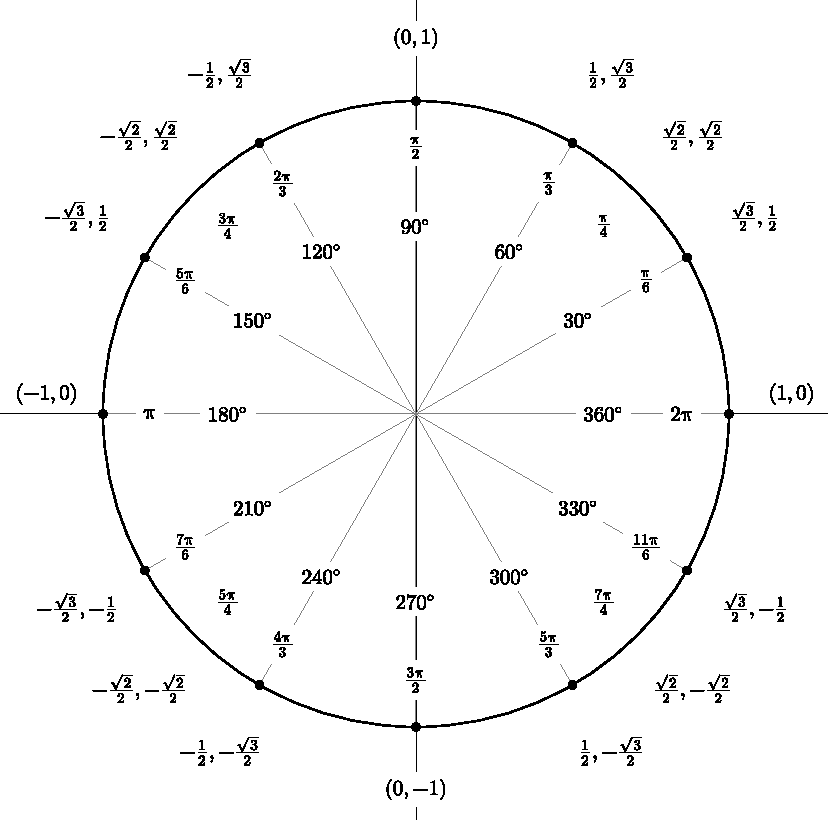
\includegraphics[width= \linewidth]{include_degrees_circle.pdf}
\end{center}

\begin{mainbox}{Trigonometrische Funktionen}
  \begin{center} 
    \begin{tabular}{c|cccccc}
      deg & 0° & 30° & 45° & 60° & 90° & 180° \\
      \midrule
      rad & 0 & $\frac{\pi}{6}$ & $\frac{\pi}{4}$ & $\frac{\pi}{3}$ & $\frac{\pi}{2}$ & $\pi$ \\
      cos & 1 & $\frac{\sqrt{3}}{2}$ & $\frac{\sqrt{2}}{2}$ & $\frac{1}{2}$ & 0 & -1 \\
      sin & 0 & $\frac{1}{2}$ & $\frac{\sqrt{2}}{2}$ & $\frac{\sqrt{3}}{2}$ & 1 & 0 \\
      tan & 0 & $\frac{1}{\sqrt{3}}$ & 1 & $\sqrt{3}$ & $+\infty$ & 0 \\
    \end{tabular}
  \end{center}
\end{mainbox}

\subsubsection{Trigonometrische Identitäten}
\begin{center}
 \begin{tabularx}{\linewidth}{>{\centering\arraybackslash}X>{\centering\arraybackslash}X}
  \toprule
  $\sin(\arccos (x))$ & $\sqrt{1-x^2}$\\
  $\cos(\arcsin(x))$ & $\sqrt{1-x^2}$\\
  $\sin(\arctan(x))$ & $\frac{x}{\sqrt{1+x^2}}$\\
  $\cos(\arctan(x))$ & $\frac{1}{\sqrt{1+x^2}}$\\
  $\tan(\arcsin(x))$ & $\frac{x}{\sqrt{1-x^2}}$\\
  $\tan(\arccos(x))$ & $\frac{\sqrt{1-x^2}}{x}$\\
  \bottomrule
 \end{tabularx}
\end{center}

\subsection{Rekursive Integrale}

$J_n = \int \frac{1}{(1 + x^2)^n} \dx$, dann $J_{n+1} = \frac{x}{2n(1 + x^2)^n} + (\frac{2n - 1}{2n})J_n$ mit $J_1 = \arctan(x)$.

\subsection{Binomischer Lehrsatz}

$$(x+y)^n = \sum_{k=0}^n {n \choose k} x^{n-k} y^k$$

\subsection{Uneigentliche Integrale}
$$\int_1^\infty \frac{1}{x^\alpha} \dx = \begin{cases}
  \text{divergiert, } & \alpha \leq 1\\
  \frac{1}{\alpha - 1} & \alpha > 1
\end{cases}$$
$$\int_0^1 \frac{1}{x^\alpha} \dx = \begin{cases}
  \text{divergiert, } & \alpha \geq 1\\
  \frac{1}{1- \alpha} & \alpha < 1
\end{cases}$$
$$\int_0^\infty e^{-x} \dx = 1$$
$$\int_0^\infty e^{-x}x^{s-1} \dx = \begin{cases}
  \text{divergiert, } & s \leq 0\\
  (s-1)! & s > 0
\end{cases}$$
$$\int_0^\infty \sin(x^2) \dx = \sqrt{\frac{\pi}{8}}$$

\subsection{Gerade und ungerade Funktionen}

Eine Funktion $f$ heisst:

\begin{itemize}
  \item gerade falls $f(t) = f(-t)$
  \item ungerade falls $f(t) = -f(-t)$
\end{itemize}

für jedes $t$ im Definitionsbereich.

\begin{itemize}
  \item Die Verknüpfung von ungeraden Funktionen ist ungerade. 
  \item Sei $g$ gerade und $f$ beliebig. $f \circ g$ ist gerade.
  \item Sei $f$ gerade und $g$ ungerade. $g \circ f$ und $f \circ g$ sind gerade.
  \item Produkt einer geraden und einer ungeraden Funktion ist ungerade.
  \item Produkt zweier ungerader Funktionen ist gerade.
  \item Produkt zweier gerader Funktionen ist gerade.
  \item Für $f: [-a, a] \to \mathbb{R}$ stetig und ungerade, d.h. $f(-x) = -f(x)$ gilt $\int_{-a}^a f(x) \dx = 0$.
\end{itemize}


\subsection{Weitere Tabellen}

\subsubsection{$n$-te Ableitungen}
\begin{center}
  \begin{tabularx}{\linewidth}{>{\centering\arraybackslash}X>{\centering\arraybackslash}X}
  \toprule
  $\mathbf{f(x)}$ & $\mathbf{f^{(n)}(x)}$ \\
  \midrule
  $\sin(x)$ & $\sin(\frac{n\pi}{2} + x)$\\
  $f + g$ & $f^{(n)} + g^{(n)}$\\
  $f \cdot g$ & $\sum\limits_{k=0}^{n}\binom{n}{k}f^{(k)}g^{(n-k)}$\\
  \bottomrule
  \end{tabularx}
\end{center}

\subsubsection{Ableitungen (I)}
\begin{center}
  \begin{tabularx}{\linewidth}{c>{\centering\arraybackslash}Xc}
  \toprule
  $\mathbf{F(x)}$ & $\mathbf{f(x)}$ & $\mathbf{f'(x)}$ \\
  \midrule
  $\frac{x^{-a+1}}{-a+1}$ & $\frac{1}{x^a}$ & $\frac{a}{x^{a+1}}$ \\
  $\frac{x^{a+1}}{a+1}$ & $x^a \ (a \ne -1)$ & $a \cdot x^{a-1}$ \\
  $\frac{1}{k \ln(a)}a^{kx}$ & $a^{kx}$ & $ka^{kx} \ln(a)$ \\
  $\ln |x|$ & $\frac{1}{x}$ & $-\frac{1}{x^2}$ \\
  $\frac{2}{3}x^{3/2}$ & $\sqrt{x}$ & $\frac{1}{2\sqrt{x}}$\\
  $-\cos(x)$ & $\sin(x)$ & $\cos(x)$ \\
  $\sin(x)$ & $\cos(x)$ & $-\sin(x)$ \\
  $\frac{1}{2}(x-\frac{1}{2}\sin(2x))$ & $\sin^2(x)$ & $2 \sin(x)\cos(x)$ \\
  $\frac{1}{2}(x + \frac{1}{2}\sin(2x))$ & $\cos^2(x)$ & $-2\sin(x)\cos(x)$ \\
  $-\ln|\cos(x)|$ & $\tan(x)$ & $\frac{1}{\cos^2(x)} = 1 + \tan^2(x)$  \\
  $\cosh(x)$ & $\sinh(x)$ & $\cosh(x)$ \\
  $\log(\cosh(x))$ & $\tanh(x)$ & $\frac{1}{\cosh^2(x)} = 1 - \tanh^2(x)$ \\
  $\ln | \sin(x)|$ & $\cot(x)$ & $-\frac{1}{\sin^2(x)}$ \\
  $\frac{1}{c} \cdot e^{cx}$ & $e^{cx}$ & $c \cdot e^{cx}$ \\
  $x(\ln |x| - 1)$ & $\ln |x|$ & $\frac{1}{x}$ \\
  $\frac{1}{2}(\ln(x))^2$ & $\frac{\ln(x)}{x}$ & $\frac{1 - \ln(x)}{x^2}$ \\
  $\frac{x}{\ln(a)} (\ln|x| -1)$ & $\log_a |x|$ & $\frac{1}{\ln(a)x}$ \\
  $\frac{1}{2}(\cosh(x)\sinh(x)+1)$ & $\cosh(x)^2$ & $2\sinh(x)\cosh(x)$\\
  $\frac{1}{2}(\sinh(x)\cosh(x) + x)$ & $\sinh(x)^2$ & $2\sinh(x)\cosh(x)$\\
  \bottomrule
  \end{tabularx}
\end{center}

\subsubsection{Weitere Ableitungen}
\begin{center}
  \begin{tabularx}{\linewidth}{>{\centering\arraybackslash}X>{\centering\arraybackslash}X}
  \toprule
  $\mathbf{F(x)}$ & $\mathbf{f(x)}$ \\
  \midrule
  $\arcsin(x)$ & $\frac{1}{\sqrt{1 - x^2}}$ \\
  $\arccos(x)$ & $\frac{-1}{\sqrt{1 - x^2}}$ \\
  $\arctan(x)$ & $\frac{1}{1 + x^2}$ \\ 
  $\text{arsinh}(x)$ & $\frac{1}{\sqrt{1 + x^2}}$ \\
  $\text{arcosh}(x)$ & $\frac{1}{\sqrt{x^2 - 1}}$ \\
  $\text{artanh}(x)$ & $\frac{1}{1 - x^2}$ \\
  $\text{arccot}(x)$ & $-\frac{1}{1 + x^2}$ \\
  $x^x \ (x > 0)$ & $x^x \cdot (1 + \ln x)$ \\
  $\cosh(x)$ & $\sinh(x)$ \\
  $\sinh(x)$ & $\cosh(x)$ \\
  \bottomrule
  \end{tabularx}
\end{center}

\subsubsection{Grenzwerte}
\begin{center}
  \begin{tabularx}{\linewidth}{XX}
    \toprule
    $\limxi \frac{1}{x} = 0$ & $\limxi 1 + \frac{1}{x} = 1$ \\
    $\limxi e^x = \infty$ & $\limxn e^x = 0$ \\
    $\limxi e^{-x} = 0$ & $\limxn e^{-x} = \infty$ \\
    $\limxi \frac{e^x}{x^m} = \infty$ & $\limxn xe^x = 0$ \\
    $\limxi \ln(x) = \infty$ & $\limxo \ln(x) = -\infty$ \\
    $\limxi (1+x)^{\frac{1}{x}} = 1$ & $\limxo (1+x)^{\frac{1}{x}} = e$ \\
    $\limxi (1+\frac{1}{x})^b = 1$ & $\limxi n^{\frac{1}{n}} = 1$ \\
    $\lim_{x\to\pm\infty} (1 + \frac{1}{x})^x = e$ & $\limxi (1-\frac{1}{x})^x = \frac{1}{e}$ \\
    $\lim_{x\to\pm\infty} (1 + \frac{k}{x})^{mx} = e^{km}$ & $\limxi (\frac{x}{x+k})^x = e^{-k}$ \\
    $\limxo \frac{a^x -1}{x} = \ln(a), \newline \forall a > 0$ &
    $\limxi x^a q^x = 0, \newline \forall 0 \le q < 1$ \\
  \end{tabularx}
  \begin{tabularx}{\linewidth}{XX}
    $\limxo \frac{\sin x}{x} = 1$ & $\limxo \frac{\sin kx}{x} = k$\\
    $\limxo \frac{1}{\cos x} = 1$ & $\limxo \frac{\cos x -1}{x} = 0$ \\
    $\limxo x \sin(\frac{1}{x}) = 0$ & $\limxo x \log x = 0$\\
    $\limxo \frac{1 - \cos x}{x^2} = \frac{1}{2}$ & $\limxo \frac{e^x-1}{x} = 1$ \\
    $\limxo \frac{x}{\arctan x} = 1$ & $\limxi \arctan x = \frac{\pi}{2}$ \\
    $\limxo \frac{e^{ax}-1}{x} = a$ & $\limxo \frac{\ln(x+1)}{x} = 1$ \\
    $\lim_{x\to 1} \frac{\ln(x)}{x-1} = 1$ & $\limxi \sqrt{x^2 + c} - x = 0$ \\
    $\limxi \sqrt[x]{x} = 1$ & $\limxi x(\sqrt[x]{n} - 1) = \ln(n)$ \\
    \bottomrule
  \end{tabularx}
\end{center}

\subsubsection{Weitere Integrale}
\begin{center}
  \begin{tabularx}{\linewidth}{>{\centering\arraybackslash}X>{\centering\arraybackslash}X}
   \toprule
   $\mathbf{f(x)}$ & $\mathbf{F(x)}$ \\
   \midrule
   $\int f'(x) f(x) \dx$ & $\frac{1}{2}(f(x))^2$ \\
   $\int \frac{f'(x)}{f(x)} \dx$ & $\ln|f(x)|$ \\
   $\int_{-\infty}^\infty e^{-x^2} \dx$ & $\sqrt{\pi}$ \\
   $\int (ax+b)^n \dx$ & $\frac{1}{a(n+1)}(ax+b)^{n+1}$ \\
   $\int x(ax+b)^n \dx$ & $\frac{(ax+b)^{n+2}}{(n+2)a^2} - \frac{b(ax+b)^{n+1}}{(n+1)a^2}$ \\
   $\int (ax^p+b)^n x^{p-1} \dx$ & $\frac{(ax^p+b)^{n+1}}{ap(n+1)}$ \\
   $\int (ax^p + b)^{-1} x^{p-1} \dx$ & $\frac{1}{ap} \ln |ax^p + b|$ \\
   $\int \frac{ax+b}{cx+d} \dx$ & $\frac{ax}{c} - \frac{ad-bc}{c^2} \ln |cx +d|$ \\
   $\int \frac{1}{x^2+a^2} \dx$ & $\frac{1}{a} \arctan \frac{x}{a}$ \\
   $\int \frac{1}{x^2 - a^2} \dx$ & $\frac{1}{2a} \ln\left| \frac{x-a}{x+a} \right|$ \\
   $\int \sqrt{a^2 - x^2} \dx $ & $\frac{a^2}{2} \arcsin(\frac{x}{a}) + \frac{x}{2} \sqrt{a^2 - x^2}$ \\
   \bottomrule
  \end{tabularx} 
 \end{center}

 \subsubsection{Trigonometrische Integrale}

 \begin{center}
  \begin{tabularx}{\linewidth}{>{\centering\arraybackslash}X>{\centering\arraybackslash}X}
   \toprule
   $\mathbf{f(x)}$ & $\mathbf{F(x)}$ \\
   \midrule
   $\int \csc(x) \dx $ & $\ln|\csc(x) + \cot(x)|$ \\
   $\int \sec(x) \dx $ & $\ln|\sec(x) + \tan(x)|$ \\
   $\int \cot(x) \dx $ & $\ln|\sin(x)|$ \\
   $\int x \sin(ax) \dx$ & $-\frac{1}{a} x \cos(ax) + \frac{1}{a^2} \sin(ax)$ \\
   \bottomrule
  \end{tabularx} 
 \end{center}

\subsubsection{Fourier-Transformationen}

\subsubsection{Laplace-Transformationen}

\begin{center}
  \begin{tabularx}{\linewidth}{c>{\centering\arraybackslash}Xc}
  \toprule
  $f(t)$ & $\mathcal{L}[f(t)](s)$ \\
  \midrule
  1 & $\frac{1}{s}, \; \Re(s) >  0$ \\
  $t^n$ & $\frac{n!}{s^{n+1}}, \; \Re(s) >  0$ \\
  $\sin(at)$ & $\frac{a}{s^2 + a^2}, \; \Re(s) >  0$ \\
  $\cos(at)$ & $\frac{s}{s^2 + a^2}, \; \Re(s) >  0$ \\
  $e^{at}$ & $\frac{1}{s-a}, \; \Re(s) >  a$ \\
  $e^{at} \sin(bt)$ & $\frac{b}{(s-a)^2 + b^2}, \; \Re(s) >  a$ \\
  $e^{at} \cos(bt)$ & $\frac{s-a}{(s-a)^2 + b^2}, \; \Re(s) >  a$ \\
  $t^n e^{at}$ & $\frac{n!}{(s-a)^{n+1}}, \; \Re(s) >  a$ \\
  $a f(t) + b g(t)$ & $a \mathcal{L}[f](s) + b \mathcal{L}[g](s)$ \\
  $t f(t)$ & $-\frac{d}{ds} \left( \mathcal{L}[f](s) \right)$ \\
  $t^n f(t)$ & $(-1)^n \frac{d^n}{ds^n} \left( \mathcal{L}[f](s) \right)$ \\
  $f'(t)$ & $s \mathcal{L}[f](s) - f(0)$ \\
  $f''(t)$ & $s^2 \mathcal{L}[f](s) - s f(0) - f'(0)$ \\
  $e^{at} f(t)$ & $\mathcal{L}[f(t)](s - a)$ \\
  $\int_0^t f(\tau) g(t-\tau) d\tau$ & $\mathcal{L}[f](s) \cdot \mathcal{L}[g](s)$ \\
  $\cosh(at)$ & $\frac{s}{s^2 - a^2}, \; \Re(s) >  a$\\
  $\sinh(at)$ & $\frac{a}{s^2 - a^2}, \; \Re(s) >  a$\\
  $\delta(t - a)$ & $e^{-as}$\\
  \bottomrule
  \end{tabularx}
\end{center}

\section{Anleitungen}

\subsection{Partialbruchzerlegung}

\begin{mainbox}{Partialbruchzerlegung}
  Seien $p(x), q(x)$ zwei Polynome. $\int \frac{p(x)}{q(x)}$ wird wie folgend berechnet:
  \begin{enumerate}
   \item Falls $\deg(p) \ge \deg(q)$, führe eine Polynomdivision durch. Dies führt zum Integral $\int a(x) + \frac{r(x)}{q(x)}$.
   \item Berechne die Nullstellen von $q(x)$.
   \item Pro Nullstelle: Einen Partialbruch erstellen.
   \begin{itemize}[left=0pt]
    \item Einfach, reell: $x_1 \to \frac{A}{x - x_1}$
    \item $n$-fach, reell: $x_1 \to \frac{A_1}{x - x_1} + \ldots + \frac{A_r}{(x-x_1)^r}$ 
    \item Einfach, komplex: $x^2 + px + q \to \frac{Ax + B} {x^2 + px + q}$
    \item $n$-fach, komplex: $x^2 + px + q \to \frac{A_1x+b_1}{x^2+px+q} + \ldots$
   \end{itemize}
   \item Parameter $A_1, \ldots, A_n$ (bzw. $B_1, \ldots, B_n$) bestimmen. ($x$ jeweils gleich Nullstelle setzen, umformen und lösen).
 
  \end{enumerate}
 \end{mainbox}

Für ein monisches Polynom $x^n + a_{n-1} x^{n-1} + \cdots + a_0 = 0$ muss jede Nullstelle $a_0$ teilen.\\

Häufig verwendete Partialbruchzerlegungen sind bspw. $\frac{1}{q(q+1)} = \frac{1}{q} - \frac{1}{q + 1}$ oder $\frac{1}{q(q-1)(q+1)} = \frac{-1}{q} + \frac{1}{2(q+1)} + \frac{1}{2(q-1)}$.

\subsection{Partielle Integration - DI Method}
Berechne $\int x^2 \cos(x) \dx = x^2 (-\frac{1}{3}\cos(3x)) - 2x(-\frac{1}{9}\sin(3x)) + 2\frac{1}{27}\cos(3x) - \int 0 \cdot \frac{1}{27} \cos(3x) \dx$.

Multipliziere Diagonal wie im Beispiel.

\begin{table}[h]
  \begin{tabular}{lll}
    & D & I \\
  + & $x^2$ & $\sin(3x)$  \\
  - & $2x$ & $-\frac{1}{3}\cos(3x)$  \\
  + & $2$ & $-\frac{1}{9}\sin(3x)$  \\
  - & $0$ & $\frac{1}{27}\cos(3x)$  
  \end{tabular}
\end{table}

Aufhören falls:
\begin{itemize}
  \item $0$ in D-Spalte.
  \item Produkt einer Reihe einfach integrierbar. Addiere oder subtrahiere je nach Reihe das Integral des Produkts.
  \item Eine Reihe wiederholt sich. Verwende Rekurrenz.
\end{itemize}

\subsection{Synthetische Division}
Berechne $\frac{6x^3 + 5x^2 - 7}{3x^2 - 2x - 1} = 2x + 3 + \frac{8x - 4}{3x^2 -2x - 1}$:\\
\begin{center}
  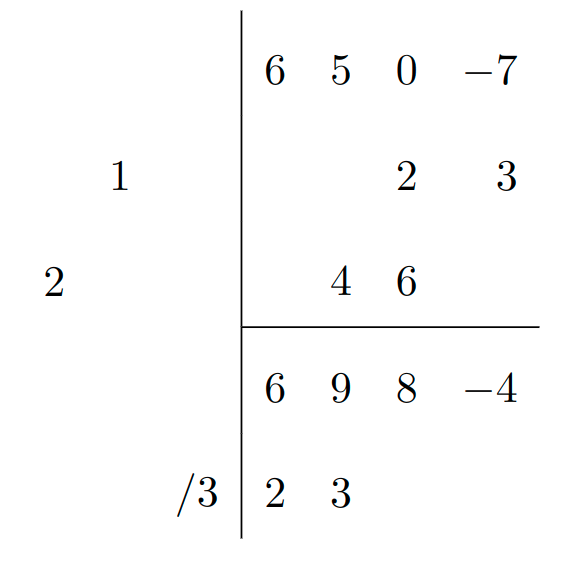
\includegraphics[width=0.4 \linewidth]{synthetic-division.png}
\end{center}



\end{document}
